\documentclass[12pt]{report}
\usepackage{suthesis-2e}
\usepackage{graphicx} %demo arg - doesn't load figs; makes rendering faster
\usepackage{apacite}
\usepackage{url}
\usepackage{booktabs}
\usepackage{pslatex}
\usepackage{setspace}
\usepackage{array,multirow}
\usepackage{tabularx} 
\doublespacing
\dept{Psychology}

\begin{document}
\title{Conceptual complexity and the evolution of the lexicon}
\author{Molly L. Lewis}
\principaladviser{Michael C. Frank}
\firstreader{Ellen M. Markman}
\secondreader{Noah Goodman}
\thirdreader{Thomas Icard} 
\fourthreader{Hyowon Gweon} 
 
\beforepreface 
\prefacesection{Abstract}
Natural languages are filled with regularities. Where do these regularities come from? A parsimonious explanation is that these regularities emerge as a consequence of pressures within the broader context in which language is used: Communication among many cognitive systems. In this dissertation, I consider one particular regularity as a case study in how the dynamics of language use might shape language structure. Specifically, I focus on a bias in natural language to map long words on to conceptually complex meanings and short words on to conceptually simple meanings, or a {\it complexity bias}. Across a series of experimental and corpus studies, I explore whether languages and their speakers have a complexity bias, what conceptual complexity is, and what pressures might have lead to this bias over the course of language evolution. In the final chapter, I consider a broader range of linguistic phenomenon and examine how aspects of language use might influence these structures. 

\prefacesection{Acknowledgments}
I feel incredibly grateful to have had the opportunity and support to study a question that I find fascinating for five years. On a short timescale, I thank the day-to-day cheer and camaraderie of the developmental community, my labmates, and my friends Kyla and Caitlin. On a longer timescale, I thank my advisor, Mike, for his intellectual guidance, but also his patience and kindness. On an even longer timescale, I thank my parents, Bonnie and Marshall, for their unconditional support of me and my pursuits. Finally, gratitude to my partner, Dan, for love and encouragement in an innumerable number of ways. This dissertation, I can say with certainty, is the product of (supportive) pressures at all of these timescales.  


%\setcounter{tocdepth}{1} TOC depth
%\FloatBarrier  % barrier to float placement of figures
%\caption[This appears in the list of figures]{This appears under the figure.} % caption in TOC vs under pic

\afterpreface

% https://github.com/samfcmc/ist-dissertation-latex-template - to make modular.
% OUTLINE: https://docs.google.com/document/d/1yaEI3AYkT3LTNtRKNAWOPFA0j6a3rUEjPA5yi8CWFGE/edit

%!TEX root = ../dissertation.tex

\chapter{Introduction}
\label{chapter:introduction}
%Chapter 1
%arbitrariness
%principles of comunication -> influence structure?
%timescales
%pragmatic equilibra in the lexicon
%accounts of the length of linguistic elements

%What is the relationship between processes at shorter timescales and language structure?

``Room for cream?'' asked the barista. ``Mm, yes -- just a bit" replied the customer. Mundane linguistic interactions such as this are the building blocks of daily experience. They are individuals making sounds to each other in an effort to coordinate their behavior in the physical world \cite{clark2006social}. These interactions are messy, variable, and highly unconstrained. Indeed it is this variability that gives language its vast expressive power \cite{hockett1960}. Yet, despite this appearance of irregularity, rich patterns in linguistic usage are revealed when we aggregate across instances of language use both within and across languages. At the level of syntax, for example, there is a strong bias in English to put subjects before verbs and, across languages, this pattern is attested more often than would be expected by chance alone  \cite{dryer2005order}. These types of probabilistic regularities exist at every level of linguistic structure --- from phonology, to semantics, syntax, and discourse --- and researchers from a variety of disciplines have taken as their project the goal of characterizing these regularities.

%Where does linguistic structure come from? \citeA[2010]{christiansen2008} propose a compelling theory. They argue that  multiple cognitive constraints dynamically influence language evolution. They suggest four constraints: the representational format of thought, properties of the percepto-motor system, learning and processing constraints, and constraints that result from reasoning about others' intentions ({\it pragmatic} constraints). Their argument is that these constraints  influence  language at the moment of use, but over time, these biases become instantiated in the structure of language. 

In this dissertation, I contribute to this effort with a particular focus on understanding on how languages use shapes language structure. I am broadly interested in how  aspects in the environment of linguistic interaction, including the cognitive system itself, can over time lead to the emergence of a regularity in the linguistic system. As a conceptual framework for exploring these dynamics, we will appeal to the notion of a {\it timescale}. A timescale is a unit of time over which significant changes in state occur. For example, the timescale of dinner is about an hour, where the significant changes in state are walking to the restaurant, sitting down, ordering food, eating the meal, then dessert, etc. In contrast, the timescale of gaining weight occurs over weeks, where the significant changes in state correspond to appreciable weight changes. Critically, the length of the timescales is determined by the change of interest. 


\begin{figure}
\begin{center} 
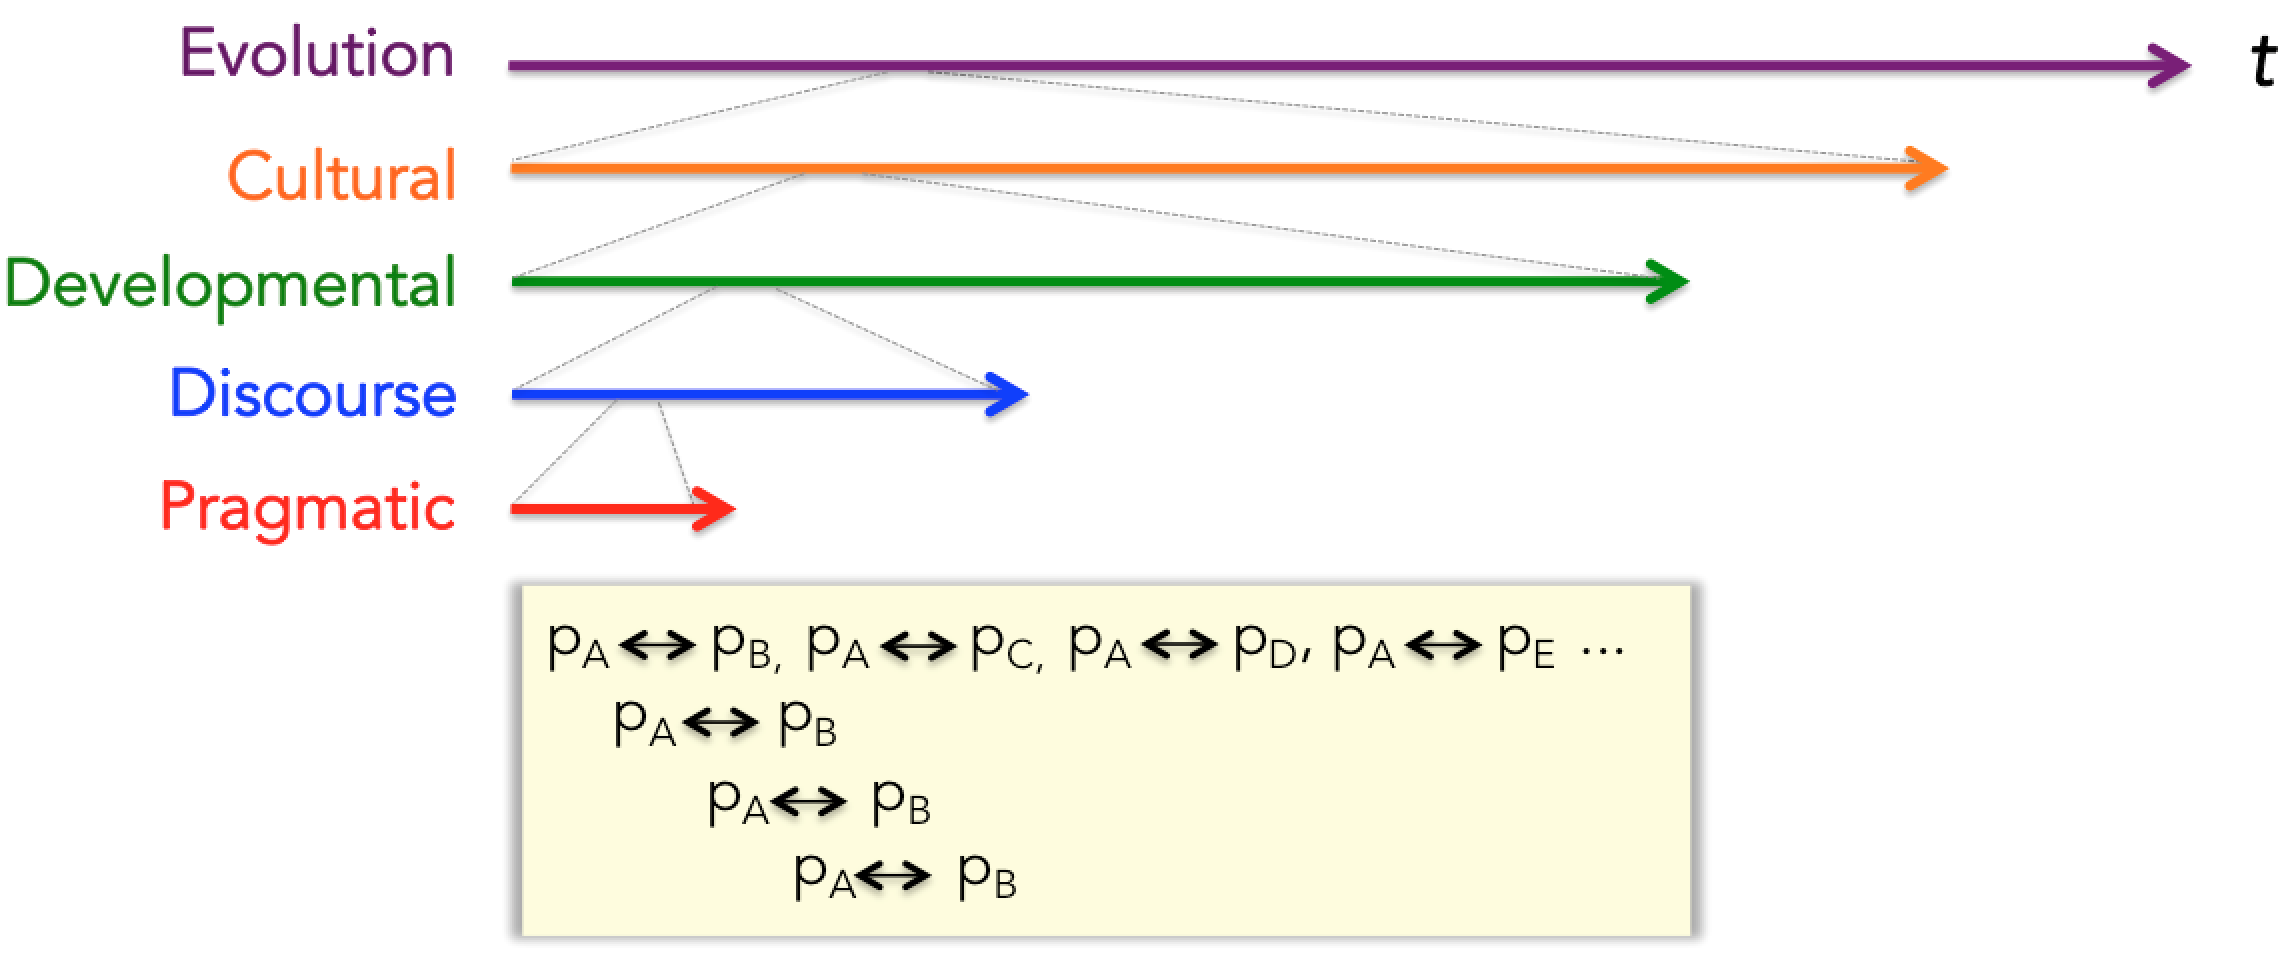
\includegraphics[width=6in]{figs/timescales1}
\caption{The five linguistic timescales. Each timescale is nested within a slice of longer timescales. The claim is that the dynamics between adjacent timescales (e.g., pragmatic and discourse) lead to changes over time in longer timescales. The developmental timescale is characterized by a particular person from a particular generation, $p_A$, interacting with a series of people over the lifespan. Repeated interactions with the same person, $p_B$, characterize the discourse timescale.}
\label{fig:timescales}
\end{center} 
\end{figure}


In the case of language, the central  hypothesis is that there are pressures at the short timescale of language use  that over long periods of time lead to changes in the structure of language. More specifically,  there are five timescales over which significant linguistic changes may occur (see Figure \ref{fig:timescales}). The first is the {\it pragmatic timescale}. The pragmatic timescale takes places over the course of the moments of communicative interaction, and corresponds to the processes  that the emerge as a consequence of reasoning about the intention of one's interlocutor, and in-the-moment pressures of the cognitive system (e.g., memory constraints).  The {\it discourse timescale} is a slightly longer timescale. The discourse timescale corresponds to repeated interactions with the same person; a series of pragmatic interactions. The third is the {\it developmental timescale}. The developmental timescale corresponds to the lifetime of an individual. It is composed of many interactions (on the pragmatic timescale), some of which with the same people (on the discourse timescale).  Many people interacting over their lifetimes lead to change at the {\it language evolution timescale}. This is the timescale over which significant changes in language structure  occur. Finally, at the longest timescale, is the {\it biological evolution timescale}. All of the dynamics at lower timescales occur within a small slice in evolutionary time. I will not have much to say about this timescale; its main significance is to situate the present claims with respect to claims about the innateness of language. Following \citeA{christiansen2008}, the suggestion is that there are aspects of language that are innate and constrain the dynamics of shorter timescales. Importantly, however, there are also  dynamics that take place at  shorter timescales, and these dynamics are the focus here.

The proposal, then, is that there are dynamics between adjacent timescales, and that, over time, these dynamics lead to change on longer timescales. Importantly, the character and phenomena of the dynamics between each pair of timescales are different. For example,  the dynamics between discourse and developmental timescales are reflected in cognitive changes in the mind of a particular speaker. In contrast, the dynamics between language evolution and biological evolution timescales are reflected in genetic changes in linguistic abilities. In Chapter 2, we review evidence suggesting a causal link between processes at the pragmatic timescale and those and the language evolution timescale.

It is worth reflecting on the historical relationship between processes at shorter timescales and language structure. Across many schools of linguistics, theorists have made a theoretical cut between language use and language structure: {\it parole} vs.\  {\it langue}  \cite{saussure},  {\it token}  vs.\  {\it type}  \cite{peirce}, and  {\it performance}  vs.\  {\it competence}  \cite{chomsky1965aspects}. These theorists  have different views on the ontological status of structure --- Saussure suggests it is a social fact, while Chomsky argues it is fundamentally a cognitive phenomenon --- but they nonetheless agree that there is some sort of invariance in language and it should be the focus of study. Language use has often been seen as an irregular, variant, and epiphenomenal to the true subject of study: structure. However, a number of more recent movements have begun to focus on language use. \nocite{labov197213} Labov's (1972) work was an important challenge to exclusionary focus on abstract structure. His work revealed systematicity in the variation of phonology as function of social variables, suggesting that ``messy" language use was governed by regularities and could therefore be studied scientifically. The study of pragmatics, more generally, can be seen as a step to find regularity in language use. 

There are, however, a number of theorists who have suggested a causal link between use and linguistic structure. One of the earliest proposals of this idea was \citeA{whorf1956language} who argued that habitual patterns of talking in particular ways (what he called ``fashions of speaking") lead over time to different conceptualizations of the world.\footnote{This is an important nuance to claims about linguistic relativity that is often over-looked: It is not {\it that} a language has a label for a concept that matters,  but rather the presence of that label in conjunction with a developmental history of using that label.} Grammar is a case where this view as been particularly well articulated, under the heading of {\it Emergent Grammar} \cite{hopper1987emergent}: 

\begin{quote} The notion of Emergent Grammar is meant to suggest that structure, or regularity, comes out of discourse and is shaped by discourse as much as it shapes discourse in an on-going process. [...] Structure, then, in this view is not an overarching set of abstract principles, but more a question of a spreading of systematicity from individual words, phrases and small sets. (p. 142)
\end{quote}
More recently, cognitive psychologists has begun to formally model these dynamics. In this tradition, \citeA{bybee2005alternatives} write: ``Properties of formal structure [...] are facts about the structure that are to be explained as arising from the cumulative impact of the processes that shape each language, as it adapts through the process of language use" (p. 406). They argue for the value of a connectionist framework in capturing these dynamics. Also within a  connectionist framework, \citeA{mcmurray2012} highlight the relevance of different timescales in capturing the phenomenon of children's word learning across the developmental timescale. Perhaps the broadest framing of these dynamics has been by \citeA{christiansen2008}, who put propose a mechanism closely aligned with the present argument.

As a case study in understanding the link between language use and language structure, the focus in this dissertation is on one aspect of language structure,  a {\it complexity bias}:
\begin{quote}
A probabilistic bias for languages to assign conceptually complex meanings to long words and conceptually simple meanings  to short words.
\end{quote}
For example, this bias predicts that a meaning with many conceptual parts, like \textsc{computer}, will be encoded linguistically with a longer label than a meaning with conceptually fewer parts, like  \textsc{hat}. The study of this particular aspect of linguistic structure is motivated by several different cognitive and communicative pressures at the pragmatic timescale could influence language use. The first is a bias to map meanings onto perceptually similar linguistic forms; that is, a bias for iconicity. There is a large body of evidence to suggest that aspects of language  contain iconic elements \cite<see>[for review]{schmidtke2014phonological}. In addition, several theories of communication---Information Theory  \cite{shannon1948} and Horn's theory communication (1984)---predict a tradeoff between length and conceptually complexity within language systems. Briefly, these two theories suggest that communication systems can maximize information transfer and minimize effort by mapping conceptually complex words to long words. We outline this prediction in more detail in the Introduction to Chapter 2.


The plan of this dissertation is as follows. In Chapter 2, we begin by examining whether languages do indeed have a complexity bias, and whether speakers have a complexity bias when faced with novel words and meanings. In this chapter, we appeal to a largely intuitive notion of conceptual complexity, assuming that objects with more physical `parts' are more conceptually complex. Across a series of ten studies we find evidence  that both languages and individual speakers have a complexity bias. In Chapter 3, we turn to the question of what conceptual complexity is more directly. Across seven studies, we explore a variety of hypotheses about the nature of conceptual complexity, ranging from the number of conceptual features a meaning has to the frequency of the object in the world. In Chapter 4, we ask how a complexity bias might come to be in the natural language over the course of language evolution. We appeal to evidence from four different studies and conclude that most evidence favors the possibility that the regularity derived from a cognitive bias for iconicity.  Finally, Chapter 5 takes a broader view on the question of how pressures of language use might shape language structure. Here we ask how a wide range of factors, across a range of timescales, might over time influence linguistic structure. 


%In this paper, I argue that we can gain  insight into the character of linguistic structure by considering the dynamics of language use. I will suggest the best way to do this is by framing language use as an instance of a broader phenomenon: social interaction \cite{clark1996using}. In particular, I will adopt the formal framework of social interaction proposed by \citeA{schelling1980strategy} in which social interactions are viewed as acts of solving coordination problems.  To illustrate, consider the barista example above. In this example, the agents are the barista and the customer, and they must coordinate how  to fill the coffee mug. There are two outcomes --- full and almost full --- and the barista's desired outcome is determined by the preference of the customer. In this case, the barista and the customer rely on language to coordinate their behavior, but this coordination could have been achieved in other ways (e.g. the customer could have shook her head, pointed to the place inside the mug that she wanted the coffee filled to, etc.). Coordination of their behavior is achieved  by arriving at the mutually preferred outcome (the customer's mug is almost full).

%A key tenet to the broader argument is that the act of using language is itself an act of solving a coordination problem \cite{clark1996using}. When a person speaks, there are many possible ways the utterance could be interpreted, and arriving at the intended interpretation is an act of coordination with the listener. For example, in the case of the customer's interaction with the barista, there are many possible interpretations of the phrase, ``Room for cream?." The barista could mean ``Would you like to add cream to your coffee? If so, I will facilitate that by not filling your mug full with coffee." Or, ``We have so much extra inventory of cream! Do you have room in your bag to take some?" Or, ``Do you like the band `Room for cream'?". Or, if the speaker is speaking another language, a totally unrelated meaning. The point is that the speaker's intended meaning is underspecified from the language form alone and the interlocutors must work collaboratively to arrive at a shared understanding. Following \citeA{lewis1969convention}, I will suggest that we can gain insight into the dynamics of linguistic coordination problems by using Schelling's formal framework.  This perspective on language use will ultimately provide a helpful framework for understanding the relationship between language use and language structure.






%!TEX root = ../dissertation.tex

\chapter{Evidence for a complexity bias}
\label{chapter:empirical}
Human languages are systems for encoding information about the world. A defining feature of a symbolic coding system is that there is no inherent mapping between the form of the code and what the code denotes \cite{peirce}---the color red holds no natural relationship to the meaning `stop', the numeral {\it 3} holds no natural relationship to three units, and in language, the word `horse' looks or sounds nothing like the four-legged mammal it denotes. This arbitrariness of the linguistic sign has long been observed as a fundamental and universal property of natural language \cite{saussure,hockett1960}. And, despite the growing number of cases suggesting instances of non-arbitrariness in the lexicon \cite<see>[for reviews]{schmidtke2014phonological,dingemanse2015arbitrariness}, there is clear evidence for at least some degree
 of arbitrariness in language based only on the observation that different languages use different words to denote the same meaning (e.g., the word for horse in English is ``horse'' but is ``at'' in Turkish).

However, the arbitrary character of language holds only from the perspective of the analyst observing a language system from the outside; from the perspective of an individual speaker, the goal of communication provides a strong constraint on arbitrariness. Perhaps this communicative constraint---roughly, that if my words were any different, I couldn't use them to talk to you---is why language doesn't \emph{seem} arbitrary to us. Put another way, Saussure's (1916, 1960) insight was an insight because the form of language typically feels just right for the use to which we put it, namely talking to other people \cite{sutherland2015explanatory}.

A rich body of theoretical work has explored communicative regularities in the use of particular forms to refer to particular types of meanings in context---the study of {\it pragmatics} \cite{grice1975logic,horn1984,clark1996using}. Broadly, this work argues that language users assume certain regularities in how speakers refer to meanings, and through these shared assumptions, the symmetry of the otherwise arbitrary character of language is broken. For example, consider a speaker who intends to refer to a particular apple on a table. Because language is {\it a priori} arbitrary, there are a range of ways the speaker could convey this meaning (e.g., ``the apple,'' ``the banana,'' ``the green apple,''``the green apple next to the plate,'' etc.), but the speaker is constrained by pragmatic pressures of the communicative context. If the listener also speaks English, the phrase ``the banana'' will be an unhelpful way to refer to the apple. Furthermore, if there is only one apple on the table, the phrase ``the green apple'' will be unnecessarily verbose given the referential context. These constraints might lead a speaker to select ``the apple'' as the referring expression, because it both allows the listener to correctly identify the intended referent while also minimizing effort on the part of the speaker.

In the present paper, we examine whether principles of communication influence the otherwise arbitrary mappings between words and meanings in the lexicon. This hypothesis is motivated by a regularity first observed by \citeA{horn1984}, who noted that pragmatic language users tend to consider the effort that speakers have exerted to convey a meaning. For example, consider the utterance ``Lee got the car to stop,'' which seems to imply an unusual state of affairs. Had the speaker wished to convey that Lee simply applied the brakes, the shorter and less exceptional ``Lee stopped the car'' would be a better description. The use of a longer utterance licenses the inference that there was some problem in stopping---perhaps the brakes failed---and that the situation is more complex.

We ask whether speakers reason the same way about the meanings of words, breaking the symmetry between two unknown meanings by reference to length. Specifically, we test the following hypotheses:

\begin{quote}
{\it Complexity Hypothesis 1}: Speakers have a bias to believe that longer linguistic forms refer to conceptually more complex meanings.

{\it Complexity Hypothesis 2}: Languages encode conceptually more complex meanings with longer linguistic forms.
\end{quote}

\noindent These two hypotheses are in principle independent from one another, and we test them separately. We see them as potentially emerging together from the same interactive forces, however, and we return to this relationship in the General Discussion.

An important construct for our hypothesis is the notion of conceptual complexity. One theoretical framework for understanding this construct is through conceptual primitives \cite<e.g.,>{locke1847}. Conceptual primitives can be thought of as the building blocks of meaning, similar to the notion of geons in the study of object recognition \cite{biederman1987}. Within this framework, a more complex meaning would be one with more primitives in it. In a probabilistic framework, having more units would also be correlated with having a lower overall probability. We adopt this framework of conceptual primitives in our working definition of complexity.

Although identifying a general set of conceptual primitives might rank among the deepest challenges for cognitive science, some work has attempted this task. A body of research has sought to understand the innate conceptual primitives in young children (``core knowledge''; Kinzler \& Spelke, 2007). \nocite{kinzler2007core} The proposed set of concepts in this work, however, is restricted to those present only  in early development (e.g., ``agent"), and is therefore not suitable for the broad scope of our current project.  Wierzbicka and colleagues (1996) have also  sought  to identify conceptual primitives, but with a more general focus.  \nocite{wierzbicka1996semantics} This work compares lexical systems across languages  to identify common primitives. The hypothesis is that there exists universal and innate semantic primitives which are the building blocks of meaning in human language. Under this view, all meanings can be derived from a set of numerable semantic primitives and a syntax for combining them. Our work here does not directly address the character of the underlying  primitives, nor whether they are universal or innate. Rather, it assumes only that such units exist for a speaker and that lexical meanings can vary in the number of their compositional primitives.

In the remainder of the Introduction, we first review prior work suggesting that communicative principles are reflected in the structure of the lexicon. We then review work related to accounts of our particular linguistic feature of interest---variability in the length of forms. Then, in the body of the paper we test the complexity hypotheses above in nine experiments and a corpus analysis.

\subsection{Pragmatic equilibria in the lexicon}

The present hypotheses are motivated by the possibility that language dynamics take place over different timescales, and these different dynamics may be causally related to each other \cite{christiansen2015now,mcmurray2012,blythe2015hierarchy}. Our two hypotheses correspond to two distinct timescales. Hypothesis 1 corresponds to the timescale of minutes in a single communicative interaction---{\it the pragmatic timescale}. Hypothesis 2 corresponds to the timescale of language change, which takes place over many years---{\it the language evolution timescale}. We consider the possibility that communicative pressures at the pragmatic timescale may, over time, influence the structure of the lexicon at the language evolution timescale. Although a complexity bias at the language evolution timescale has not been previously explored, there are a number of other cases in which pragmatic equilibria are reflected in the structure of the lexicon. Here, we describe three such cases: semantic organization, ambiguity, and one-to-one structure.

Several broad theories of pragmatics include a version of two distinct pressures on communication: the desire to minimize effort in speaking ({\it speaker pressure}) and the desire to be informative \cite<{\it hearer pressure;}>{zipf1936,horn1984}. Importantly, these two pressures trade off with each other: The optimal solution to the speaker's pressure is a single utterance that can refer to all meanings, while the optimal solution to the hearer's pressure is a longer utterance that presents no ambiguity. The utterance that emerges is argued to be an equilibrium between these two tradeoffs.\footnote{Note that this analysis only reflects interlocutors' {\it non}-aligned utilities in a communication task. Of course, both speaker and hearer also have aligned utility derived from successful communication.}

At the timescale of language evolution, there are a number of cases in which these pragmatic equilibria are reflected in the lexicon. The most well-studied of these cases is the size of the semantic space denoted by a particular word. Horn (1984) argues that the hearer has a pressure to narrow semantic space. This reflects the idea that the hearer's optimal language is one in which every possible meaning receives its own word. To understand this, consider the word ``rectangle,'' which refers to a quadrilateral with four right angles. A special case of a ``rectangle'' is a case where the four sides are equal in length, which has its own special name, ``square.'' Consequently, the term ``rectangle'' has been narrowed to mean a quadrilateral with four right angles, where the four sides are {\it not} equal. From the speaker's perspective, there is a pressure for semantic broadening. This is because the speaker's ideal language is one in which a single word can refer to a wide range of meanings. This phenomenon is exemplified by the broadening of brand names to refer to a kind of product. For example, ``kleenex'' is a product name for facial tissues, but has taken on the meaning of facial tissues more generally.

The opposition of these two semantic forces predicts an equilibrium in the organization of semantic space that satisfies the pressures of both speaker and hearer. A growing body of empirical work tests this prediction by examining the organization of particular semantic domains cross-linguistically \cite<see>[for review]{regierword}. This work finds that languages show a large degree of similarity in how they partition semantic space for a particular domain, but also a large degree of variability. Such analyses demonstrate that the attested systems all approximate an equilibrium point between hearer and speaker pressures.

 In one example of this kind of analysis, \citeA{kemp2012kinship} demonstrate this systematicity in the semantic domain of kinship. For each language, they developed a metric of the degree to which Horn's speaker and hearer pressures are satisfied. A language that better satisfies the hearer's pressure is one that is more complex, as measured by the description length of the system in their representational language. A language that better satisfies the speaker's pressure is one that requires less language to describe the intended referent. To understand this, consider the word ``grandmother'' in English: This word is ambiguous in English because it could refer to either the maternal or paternal mother, and so identifying which mother the speaker is referring to is more costly in English than in a language that encodes this distinction lexically. They find that the set of attested languages is a subset of the range of possible languages, and this subset partitions the semantic space in a way that near optimally trades off between pragmatic pressures. This type of analysis has also been performed for the domains of color \cite{regier2007color}, lightness \cite{baddeley2009}, and numerosity \cite{xu4numeral}.

A second phenomenon that is predicted by these pressures is the presence of multiple meanings associated with the same word, or lexical ambiguity. Lexical ambiguity is present in  many open-class words like ``bat'' (a baseball instrument or a flying mammal). Lexical ambiguity is tolerated because the meaning is usually easily disambiguated by context. When the word ``bat'' is uttered while watching a baseball game, the mammal usage of the word is very unlikely. The presence of this type of ambiguity can be viewed as an equilibrium between the two pragmatic pressures: If the meaning of a word can be disambiguated by the referential context, then it would violate the speaker's pressure to minimize effort by keeping track of two distinct words.

Indeed, recent work by \citeA{piantadosi2011b} reveals systematicity in the presence of lexical ambiguity in language. They argue that ambiguity results from a speaker based pressure to broaden the meaning of a word to include multiple possible meanings. In particular, they suggest that this pressure should lead to a systematic relationship between the presence of ambiguity and the cost of a word. According to their argument, costly words (in terms of length, frequency, or any metric of cost) that are easily understood by context violate the speaker's principle to say no more than you must. Consequently, there should be a pressure for these meanings to get mapped on to a different, less costly word. This word may happen to already have a meaning associated with it, and so the result is multiple meanings being mapped to a single word. For example, in the case of the word ``bat,'' a speaker could instead say ``baseball bat.'' But, because this referent is easily disambiguated in context from the mammalian meaning, a speaker pressure should result in the use of the shorter form. This logic leads to a testable prediction: that shorter words should tend to be more ambiguous. Through corpus analyses, \citeA{piantadosi2011b} find this precise relationship between cost and ambiguity. Across English, Dutch and German, they find that shorter words are more likely to have multiple meanings.

An additional case of this lexical ambiguity is found in words that have very little context-independent meaning, known as indexicals or deictics \cite{frawley2003international}. These words get their meaning from the particular referential context of the utterance, and are therefore highly ambiguous from a context-independent perspective. There are many types of indexicals that are present to varying degrees across languages. Consider the temporal indexical form ``tomorrow.'' The context-independent meaning of this word is something like ``the day after the day this word is being uttered in.'' Critically, abstracted from any context, this word has little meaning; it is impossible to interpret without having knowledge about the day the word was uttered. This phenomenon is also present in person pronouns (e.g., ``you'' and ``I'') and spatial forms, like ``here'' and ``there.'' As for lexical ambiguity, this type of ambiguity is a predicted equilibrium point from Horn's principles: If the hearer can recover the intended referent from context, the speaker would be saying more than is necessary by using an overly-specific referential term (e.g., ``December 18th, 2014'' vs.``tomorrow''). Indexicals, therefore, provide another instance of ambiguity in lexical systems, which may emerge as an equilibrium from the speaker's pressure to minimize effort. 

Finally, the relationship between the meanings of different words can be seen as a consequence of pragmatic principles. A number of theorists have noted a bias against two words mapping onto the same meaning --- that is, a bias against synonymy \cite{saussure,kiparsky1983word,horn1984,clark1987principle,clark1988logic}. This bias is an equilibrium between Horn's speaker and hearer principles. Recall that the optimal language for a speaker is one in which a single word maps to all meanings, and the optimal language for a hearer is one in which each word maps to its own meaning. Synonymy biases language toward neither of these ideals; it only results in more words for both the speaker and the hearer to keep track of.  Thus, when a listener hears a speaker use a second word for an existing meaning, the hearer infers that this could not be what the speaker intended because this would violate the speaker's principle. The result is  an assumption that the second word maps to a different meaning and, ultimately, a language structure that is biased against synonymy.

As one kind of evidence for this one-to-one structure in the lexicon, \citeA{horn1984} points to a phenomenon called {\it blocking}. Blocking refers to cases in which an existing lexical form blocks the presence of a different, derived form with the same root. Consider the following examples:
 \begin{quote}
 	(a) fury furious *furiosity\\
	(b) *cury curious curiosity
\end{quote}
In both (a) and (b), forms that would be expected, given the inflectional morphology in English, are not permitted. This is because the common root would lead to an overlap in meaning. Examples such as this provide some evidence for a one-to-one structure in language, but a one-to-one structure is a particularly difficult linguistic regularity to test empirically. Nonetheless, it is an important regularity because it licenses certain inferences in interpreting the meaning of words. In particular, the cognitive representation of a lexical one-to-one regularity---{\it mutual exclusivity}---has been posited as a powerful bias in children's word learning \cite{markman1988,markman2003}.

Together these phenomena---semantic organization, ambiguity, and one-to-one structure---provide three cases in which equilibria that are predicted by theories of communication at the pragmatic timescale are reflected in the structure of the lexicon at the language evolution timescale. While this similarity across timescales does not entail causality, it is suggestive of a causal relationship between the two timescales. Next, we turn to accounts at both the pragmatic and language evolution timescale for our linguistic feature of interest: length.

\subsection{Accounts of the length of linguistic elements}

Language forms vary along many dimensions, but a salient dimension is length: words and entire utterances can have dramatically different phonetic lengths. Researchers have studied this variability at both the pragmatic timescale (utterances) and the language evolution timescale (words). Our two hypotheses propose that variability at both timescales is related to the conceptual complexity of meaning. Here, we review existing work at both timescales that attempts to account for variability in language length. At the pragmatic timescale, three theories suggest that pragmatic pressures influence the length of utterances: Zipf's theory of communication, Horn's theory of communication, and Information Theory. Hypothesis 1 falls directly out of both Horn's theory of communication and Information Theory. At the language evolution timescale, two bodies of work account for word length by appealing to the predictability of the linguistic context and the conceptual `markedness' of meaning. While distinct from Hypothesis 2, both of these literatures are consistent with the proposal that languages use longer words to encode conceptually more complex meanings.

\citeA{zipf1936} provided an early account of word length that appealed to a pragmatic pressure to communicate efficiently. He argued that speakers are motivated to minimize their physical effort and that this constraint could be optimally minimized by using shorter words for meanings that were used to more frequently. This leads to the prediction that there should be an inverse relationship between the length of a word and its frequency in usage---and, indeed, the empirical data suggest a robust correlation between word length and word frequency.

Others, however, have proposed different pressures at the pragmatic timescale that might influence the length of linguistic expressions. Both Horn's theory of communication and information theory predict that longer expressions should be associated with less predictable or typical meanings than their shorter counter parts. Under Horn's theory (1984), a speaker often has the choice of using two different utterances to refer to the same meaning (in truth conditional terms), and often these utterances differ in length. Horn suggests that the sentences ``Lee stopped the car.'' and ``Lee got the car to stop'' have the same denotational meaning (the successful stopping of a car), though they differ in length. The claim is that this asymmetry leads to an inference on the part of the listener that the two differ in meaning.

The logic of this inference is identical to the lexical structure case above. The listener hears a speaker use a more costly phrase to express a meaning that could have been expressed in a less costly way. The listener thus infers that this other meaning could not be what the speaker intended because this would violate the speaker's principle to say no more than is necessary. Horn adds an additional layer to this argument. He suggests that not only do these two forms differ in meaning, but that they map onto meanings in a systematic way: The longer form gets mapped on to the more unusual meaning, while the shorter form refers to the more usual meaning. Thus, in the above example, the shorter utterance would refer to a simple, average case of car stopping, while longer utterance might refer to case where something complex or unusual happened, perhaps because Lee used the emergency brake.

The source of the particular mapping between forms of different lengths and meanings is unclear. This is because in principle there are multiple equilibrium points in the mapping between form and meaning. Assuming a one-to-one constraint on the mapping, there are two possible equilibria: \{short--simple, long--complex\} or \{short--complex, long--simple\}. Both satisfy the constraint that each form gets mapped to a unique meaning. So how do speakers arrive at the \{short--simple, long--complex\} equilibrium? \citeA{bergen2014} successfully derive this result as a consequence of the fact that \{short--simple, long--complex\} is a more optimal mapping for the speaker. Another possibility relies on iconicity: Hearers have a cognitive bias to map more complex sounding forms to meanings that are similarly complex.

 \citeA{bergen2012} provide a direct test of the length-complexity tradeoff within a communication game. In their task, partners were told that they were in an alien world with three objects and three possible utterances. In this experiment, the idea of complexity was operationalized as frequency, such that participants were instructed that each of the three different objects had three different base rate frequencies associated with them. The cost of the utterance was manipulated directly (rather than through utterance length) by assigning different monetary costs to each object. Participants' task was to communicate about one of the objects using one of the available utterances. If they successfully communicated, they received a reward. The results suggest that both the speaker and hearer expected costlier forms to refer to less frequent meanings, consistent with Horn's predicted equilibrium between word length and meaning.

The prediction of a complexity bias at the pragmatic timescale falls more directly out of information theory. Information theory models communication as the transfer of information across a noisy channel \cite{shannon1948}. Under this theory, speakers optimize information transfer (in terms of bits) by keeping the amount of information conveyed in a unit of language constant across the speech stream. A straightforward consequence of this {\it uniform information density} assumption is that speakers should try to lengthen unpredictable utterances. There is evidence for this prediction across multiple levels of communication. At that level of prosody, speakers tend to increase the duration of a word in cases where the word is unpredictable (highly informative) given the local \cite{aylett2004smooth} and global \cite{seyfarth2014word} linguistic context. There is also evidence for this prediction at the level of syntactic \cite{frank2008speaking} and discourse predictability \cite{genzel2002entropy}.

At the timescale of language evolution, there is some indirect evidence that this same bias is present in the lexicon. These approaches use the linguistic context of a word as a measure of the complexity of meaning. The idea is that words that are highly predictable, given the linguistic context, have more complex meanings, while words that are less predictable given the linguistic context, have less complex meanings. \citeA{piantadosi2011a} measured the relationship between the predictability of a word in context and its length. Across 10 languages, these two measures were highly correlated: words that were longer were less predictable in their linguistic context on average. This result held true even controlling for the frequency of words. Additional evidence for this relationship comes from examining pairs of words that have very similar meaning, but differ in length \cite<e.g. ``exam'' vs.\ ``examination;''>{mahowald2012info}. In corpus analyses, longer forms are found to be used in less predicable linguistic contexts. They also find in a behavioral experiment that speakers are more likely to select the longer alternative in less predictive contexts. This body of work points to a systematic relationship between word length and meaning when complexity is operationalized as predictability in the linguistic context.

A related body of work has examined the relationship between length and meaning under the rubric of {\it markedness}, or iconicity more broadly \cite{jakobson1966quest}. While many notions of iconicity have been discussed in the literature \cite{haspelmath2006against,haspelmath2008frequency}, one version of the hypothesis is that linguistic forms often have binary morphemic contrasts and these contrasts map onto a broad difference in meaning \cite{greenberg1966}. For example, consider the pair ``real''--``unreal,'' which differ both in valence---positive vs.\ negative---and length (the negative form has the extra morpheme ``un-''). \citeA{greenberg1966} suggests that the difference in length is because negative meanings are conceptually more marked than their positive counterparts, and that this regularity is a linguistic universal. One explanation of this is that the set of negated things tends to be larger than the set of positive things (in principle, there are more unreal things than real things). However, a limitation of this proposal is that there is no {\it a priori} criteria for determining what characterizes conceptual markedness; the accounts are specific to each domain. For example, while the negation case appeals to `number of things' as the determiner of complexity, there is no clear account of why the present form (e.g.\ ``walk'') should be less marked than the past  form (e.g.\ ``walked'') or why state words (e.g.\ ``black'') should be less marked than change of state words (e.g.\ ``blacken''). Nonetheless, this version of the markedness hypothesis suggests a relationship between linguistic length and conceptual features, similar to the complexity hypothesis. 

The complexity hypothesis differs from this prior work in several ways.  First, we propose conceptual complexity as a general construct that can be applied to a broad class of meanings. The hypothesis also differs in the specificity of the length metric: While markedness predicts a regularity only at the level of morphemes, the complexity hypothesis predicts a regularity at all levels of linguistic form (phonemes, syllables, morphemes). Finally, the complexity hypothesis provides an operationalization of iconicity that allows for a more direct test of the mechanism underlying systematicity between length and meaning.  \citeA{haspelmath2008frequency} argues that the systematicity between length and meaning is not the result of a cognitive bias related to the meaning of the word, but rather due to differences in frequency of use. By providing a general definition of complexity, we are able to test for systematicity between word meaning and length, independent of frequency. 

Thus, at the pragmatic timescale, there is a well-motivated prediction that less predictable meanings should be described with longer utterances. If dynamics at shorter timescales influence those at longer timescales, we might expect this same regularity to emerge in the lexicon over the course of language evolution. At the language evolution timescale, there is some indirect evidence that longer words refer to more complex meanings, but no work directly and systematically tests this prediction.

\subsection{Our studies}

The goal of our work here is to test the two complexity hypotheses given above. We present ten studies that provide support for both hypotheses: a complexity bias in individual speakers (Hypothesis 1; Experiments 1-8) and a complexity bias in natural language (Hypothesis 2; Experiments 9-10; see Table~\ref{exp_summary_table} for a summary of our studies). In Experiments 1-7, we test whether participants are biased to map a relatively long novel word onto a relatively more complex object, using artificial objects (Experiments 1-3) and novel, real objects (Experiments 4-7). In Experiment 8, we explore the underlying cognitive construct of complexity in a reaction time task. In Experiment 9, we elicit complexity norms for English words and then conduct a corpus analysis of 79 additional languages (Study 10). In these studies, we operationalize the notion of conceptual complexity by manipulating it visually and also measuring it, both directly through explicit norms and indirectly through reaction time. Each approach to operationalization appeals to a broad definition of complexity where more complex meanings are assumed to have more `parts.' In the General Discussion, we  summarize the support these studies provide for our hypotheses as well as their limitations and directions for future work.

%\onehalfspacing
\begin{table}[t]
\footnotesize
\centering
\begin{tabular}{l l l l l }
 \toprule
 \textbf{Experiment} &  \textbf{Description} & \textbf{\begin{tabular}[c]{@{}l@{}}Complexity\\Hypothesis \end{tabular}}&  \textbf{Stimulus Type} \\
 \toprule

1 & Explicit complexity norms & 1  & artificial objects  \\
2 & Mapping task & 1 & artificial objects    \\
3  & Mapping task (control)  & 1 & artificial objects   \\
4  & Explicit complexity norms & 1 & novel real objects   \\
5  & Mapping task & 1 & novel real objects \\
6 & Mapping task (control) & 1  & novel real objects    \\
7  & Label production& 1 & novel real objects  \\
8  & Memory task to elicit RTs & 1 & artificial (a) and novel real (b) objects\\
9   & English complexity norms & 2 & real words \\
10  & Cross-linguistic corpus analysis & 2   & real words \\
 \bottomrule
\end{tabular}
\caption{Summary of studies.}
\label{exp_summary_table}
\end{table}
%\doublespacing

\section{Experiment 1: Object Complexity Norms (Artificial Objects)}
\label{ch2-1}

As a first step in exploring a complexity bias, we manipulated the complexity of objects and asked participants to infer which object a novel word refers to. Object complexity was manipulated by varying the number of primitive parts the objects were composed of. If participants have a complexity bias, we predicted they should be more likely to map a longer novel word onto an object composed of more parts, compared to an object with fewer parts. In Experiment 1, we first conducted a norming study to verify our intuitions that the number of object parts correlated with explicit judgements of complexity. In Experiment 2, we used these normed stimuli in a simple word mapping task, revealing a complexity bias. Experiment 3 replicated Experiment 2 with randomly concatenated syllables.


\subsection{Methods}

\subsubsection{Participants} In this and all subsequent experiments, participants were recruited on Amazon Mechanical Turk and received US \$0.15-0.30 for their participation, depending on the length of the task. 60 participants completed this first experiment.

Across all experiments, some participants completed more than one experiment. The results presented here include the data from all participants, but all reported results remain reliable when excluding participants who completed more than one study. Participants were counted as a repeat participant if they completed a study using the same stimuli (e.g., completed both Experiment 1 and 2 with artificial objects).

\subsubsection{Stimuli}
As object primitives, we used ``geon'' shapes which are argued to be primitives in the visual system under one theory of object recognition \cite{biederman1987}. We created a set of 40 objects containing 1-5 geon primitives (Figure \ref{fig:geons}).\footnote{All stimuli, experiments, raw data and analysis code can be found at \url{https://github.com/mllewis/RC}.
Analyses can be found at: \url{https://mllewis.github.io/projects/RC/RCSI.html}.}

\begin{figure}
 \begin{center}
  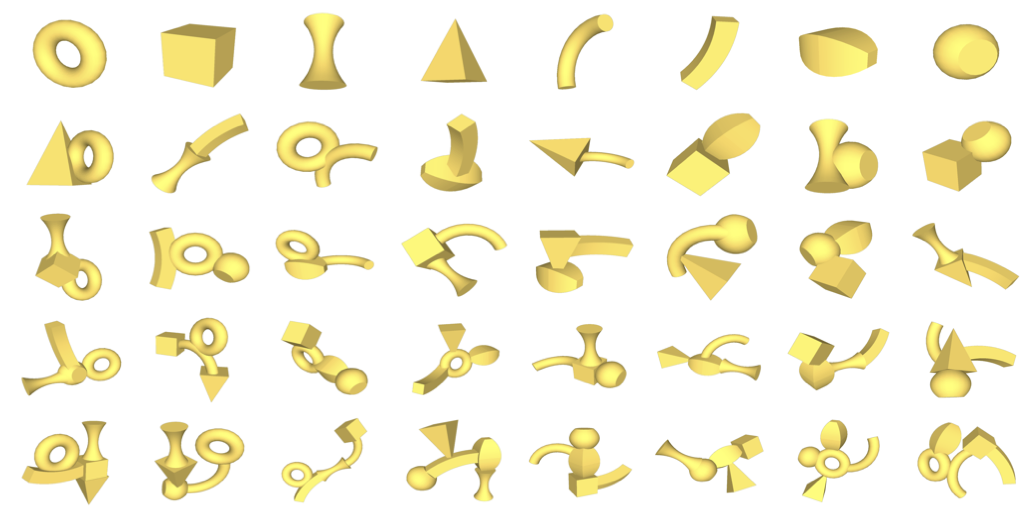
\includegraphics[height=2in]{figs/geon_stimuli.png}
  \caption{\label{fig:geons} Artificial objects used in Experiment 1. Each row corresponds to a complexity condition. The complexity condition is determined by the number of ``geon'' parts the object contains (1-5). }
 \end{center}
\end{figure}

\subsubsection{Procedure}
We presented participants 12 objects from the full stimulus set one at a time. For each object, we asked ``How complicated is this object?,'' and participants responded using a slider scale anchored at ``simple'' and ``complicated.'' Each participant saw two objects from each complexity condition, and the first two objects were images of a ball and a motherboard to anchor participants on the scale. This and all subsequent experimental paradigms can be viewed directly here: \url{https://mllewis.github.io/projects/RC/RCindex.html}.

\subsection{Results and Discussion}
Number of object parts was highly correlated with explicit complexity judgment ($r = .93$, $p < .0001$; $M = .47$, $SD = .18$): Objects with more parts tend to be rated as more complex.\footnote{We are interested in the relationship between measurements (specifically, word length and complexity), rather than participant-wise variability. We therefore conduct most of our analyses on item means. All correlations reported are at the item level, with the exception of Experiments 2 and 5 where we report the correlation across effect sizes. In Experiments 3, 6 and 7, we use linear mixed effect models due to the repeated-measure design in these experiments.} Figure \ref{fig:study1_plots}a shows the mean complexity rating for each of the 40 objects as a function of their complexity condition. This finding suggests that we can use manipulations of visual complexity as a proxy for manipulations of conceptual complexity.

\begin{figure}[t]
 \begin{center}
  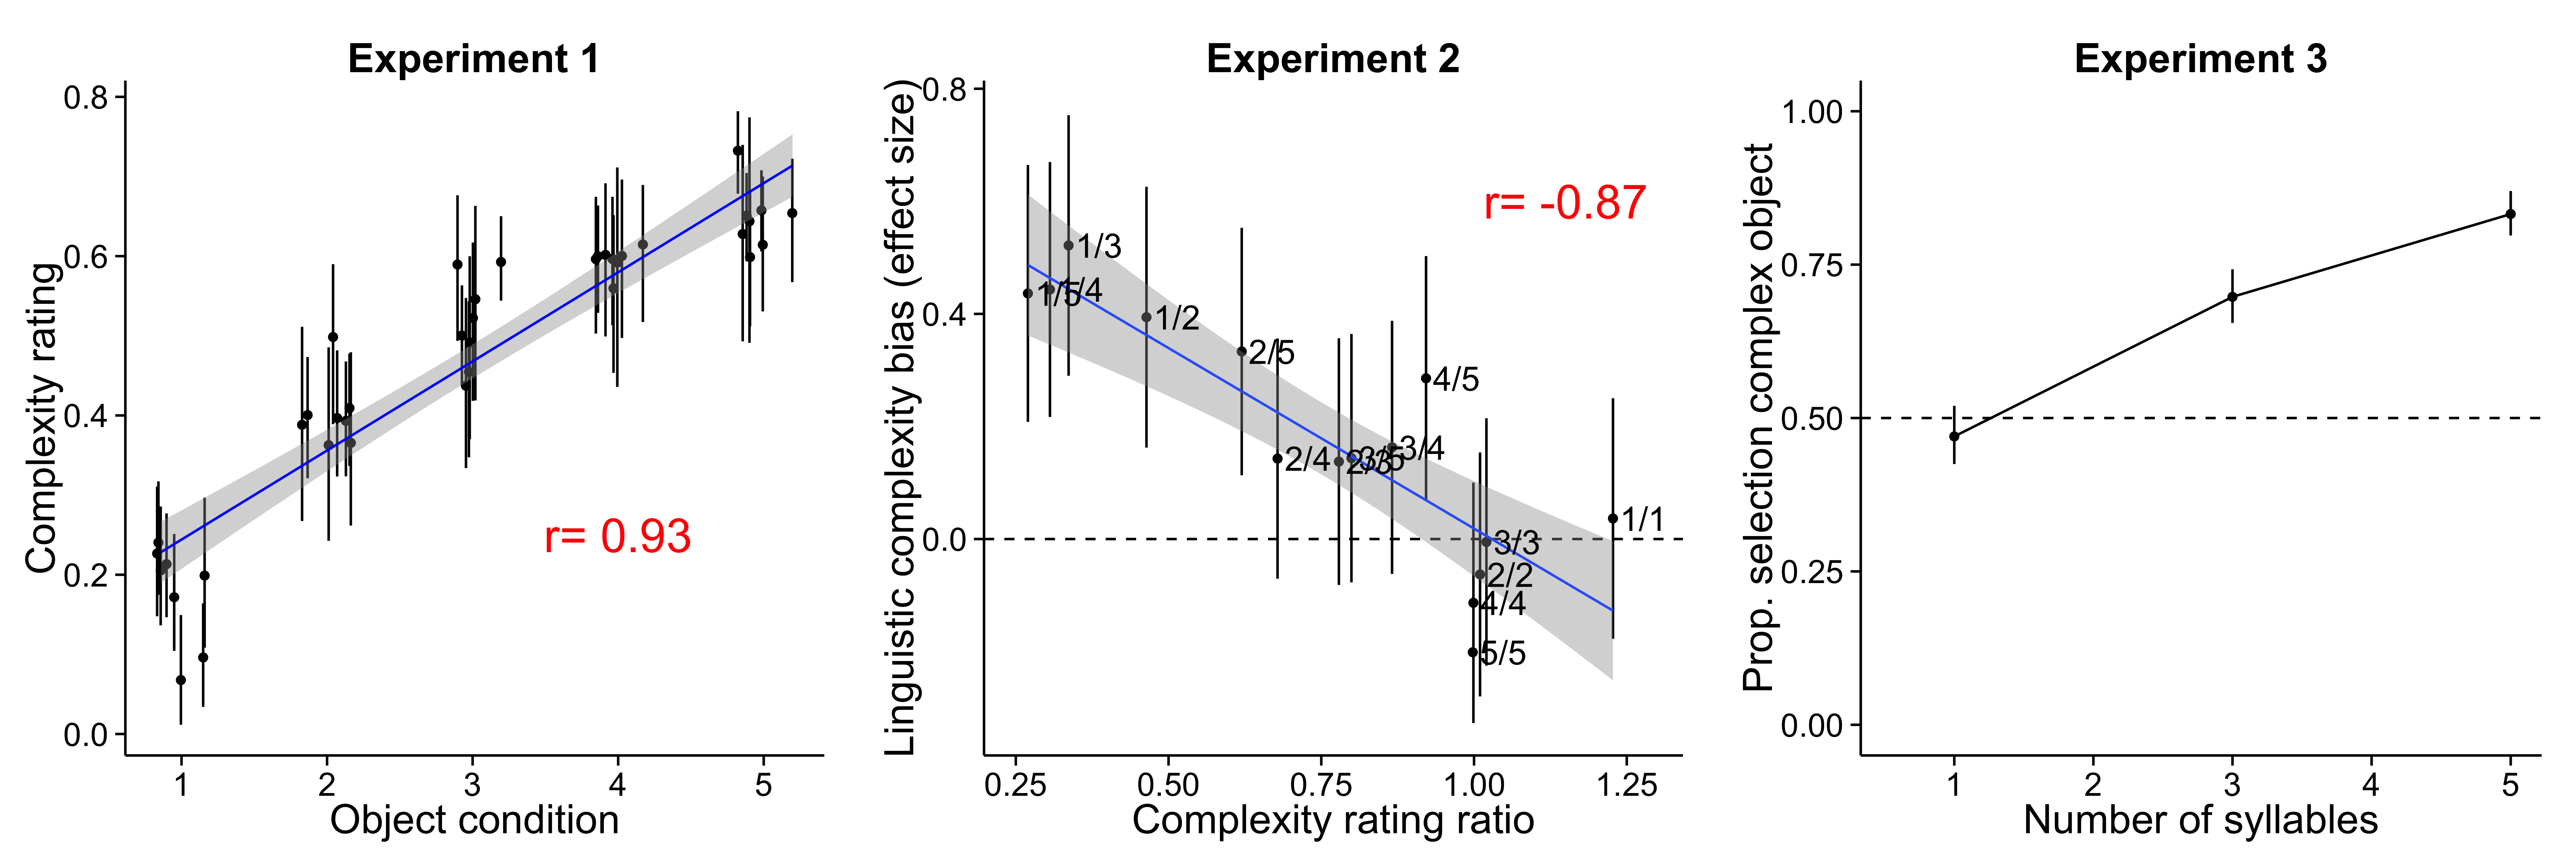
\includegraphics[width=6in]{figs/study1_plots.png}
  \caption{ \label{fig:study1_plots} (a) The relationship between number of geons and complexity rating is plotted below. Each point corresponds to an object item (8 per condition). The x-coordinates have been jittered to avoid over-plotting. (b) Effect size (bias to select complex alternative in long vs.\ short word condition) as a function of the complexity rating ratio between the two object alternatives. Each point corresponds to an object condition. Conditions are labeled by the number of geons of the two alternatives. For example, the ``1/5'' condition corresponds to the condition in which one alternative contains 1 geon and the other contains 5 geons. (c) Proportion complex object selections as a function of the number of syllables in the target label. The dashed line reflects chance selection between the simple and complex alternatives. All errors bars reflect 95\% confidence intervals, calculated via non-parametric bootstrapping in 1a and 1c, and parametrically in 1b.
 }
 \end{center}
\end{figure}


\section{Experiment 2: Mapping Task (Artificial Objects)}


\subsection{Methods}
\subsubsection{Participants} 750 participants completed the experiment.
\subsubsection{Stimuli}
The referent stimuli were the set of 40 objects normed in Experiment 1. The linguistic stimuli were novel words either 2 or 4 syllables long (e.g., ``bugorn'' and ``tupabugorn''). There were 8 items of each syllable length.

\subsubsection{Procedure}

We presented participants with a novel word and two possible objects as referents, and asked them to select which object the word named (``Imagine you just heard someone say {\it bugorn}. Which object do you think {\it bugorn} refers to? Choose an object by clicking the button below it.'').

Within participants, we manipulated word length and the relative complexity of the referent alternatives. We tested every unique combination of object complexities (1 vs.\ 2 geons, 1 vs.\ 3 geons, 1 vs.\ 4 geons, etc.), giving rise to 15 conditions in total. Each participant completed 4 short and 4 long trials in a random order, where each word was randomly associated with one of the complexity conditions. No participant saw the same complexity condition twice and no word or object was repeated across trials.

\subsection{Results and Discussion}
Across conditions, the more complex object was more likely to be judged the referent of the longer word. For each object condition (e.g., 1 vs.\ 2 geons), we calculated the effect size for participants' complexity bias---the degree to which the complex object was more likely to be chosen as the referent of a long word, compared to the short word. Effect sizes were calculated using the log odds ratio \cite{sanchez2003effect}. Effect size was highly correlated with the ratio of object complexities: The greater the mismatch in object complexity, the more the longer word was paired with the more complex object ($r = -.87$, $p < .0001$). This experiment thus provides initial evidence for a complexity bias in the lexicon: Given an artificial word and two objects of differing visual complexity, participants are more likely to map a longer word onto a more complex referent, relative to a shorter word.


\section{Experiment 3: Control Mapping Task (Artificial Objects)}
One limitation of Experiment 2 is that it uses a small set of words as the linguistic stimuli (8 short and 8 long), making it possible that idiosyncratic properties of the words could be driving the observed complexity bias. In Experiment 3, we sought to test this possibility by using words composed of randomly concatenated syllables rather than items selected from a small list of words. The design was identical to Experiment 2, except that we tested only the most extreme complexity condition, the ``1/5'' condition.

\subsection{Methods}
\subsubsection{Participants} 200 participants completed the experiment.
\subsubsection{Stimuli} The referent stimuli were the geon objects composed of either 1 or 5 geons. The novel words were created by randomly concatenating 1, 3, or 5 consonant-vowel syllables. The last syllable of all words ended in a consonant to better approximate the phonology of English (e.g., ``nur,'' ``nobimup,'' ``gugotobanid'').

\subsubsection{Procedure}
Participants completed six forced-choice trials identical to Experiment 1b. We tested only the ``1/5'' complexity condition (1-geon object vs.\ 5-geon object). Word length was manipulated within-participant such that each participant completed 2 trials for each of the three possible word lengths (1, 3, or 5 syllables).

\subsection{Results and Discussion}
To examine the effect of length on referent selection, we constructed a generalized linear mixed-effect modeling predicting referent selection with word length. We included random by-participant intercepts and slopes. Replicating the ``1/5'' condition in Experiment 2, we found that participants were more likely to select a five geon object compared to a single geon object as the number of syllables in the word increased ($\beta=-.60$, $z =-8.63$, $p <.0001$). This finding suggests that the complexity bias observed in Experiment 2 is unlikely to be due to the particular set of words we selected.

\section{Experiment 4: Object Complexity Norms (Novel Objects)}
\label{ch2-4}

Experiments 1-3 provide evidence for a complexity bias using artificial objects. The complexity manipulation in these experiments was highly transparent, however, making it possible that task demands influenced the effect. We next asked whether this bias extended to more naturalistic objects where the variability in complexity might be less obvious to participants. We conducted the same set of 3 experiments as above using a sample of real objects without canonical labels. We find that the complexity bias observed with artificial geon objects extends to naturalistic objects.

\subsection{Methods}
\subsubsection{Participants} We recruited two samples of 60 participants to complete Experiment 4.

\subsubsection{Stimuli}
We collected a set of 60 objects that were real objects but that we judged not to have canonical labels associated with them (Figure \ref{fig:realobjs}).

\begin{figure}
 \begin{center}
  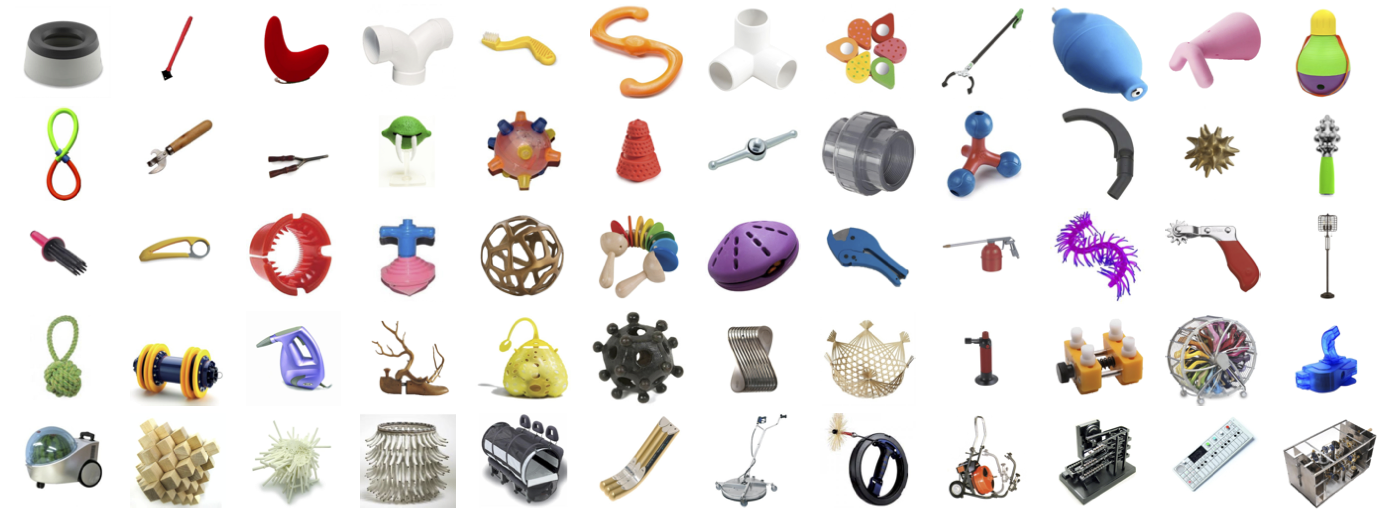
\includegraphics[height=2in]{figs/realobjs_stimuli.png}
  \caption{\label{fig:realobjs} Novel real objects used in Experiments 4-6: Naturalistic objects without canonical labels. Each row corresponds to a quintile determined by the explicit complexity judgments obtained in Experiment 4 (top: least complex; bottom: most complex).}
 \end{center}
\end{figure}

\subsubsection{Procedure} The procedure was identical to Experiment 1.

\subsection{Results and Discussion}

 \begin{figure} [t]
 \begin{center}
  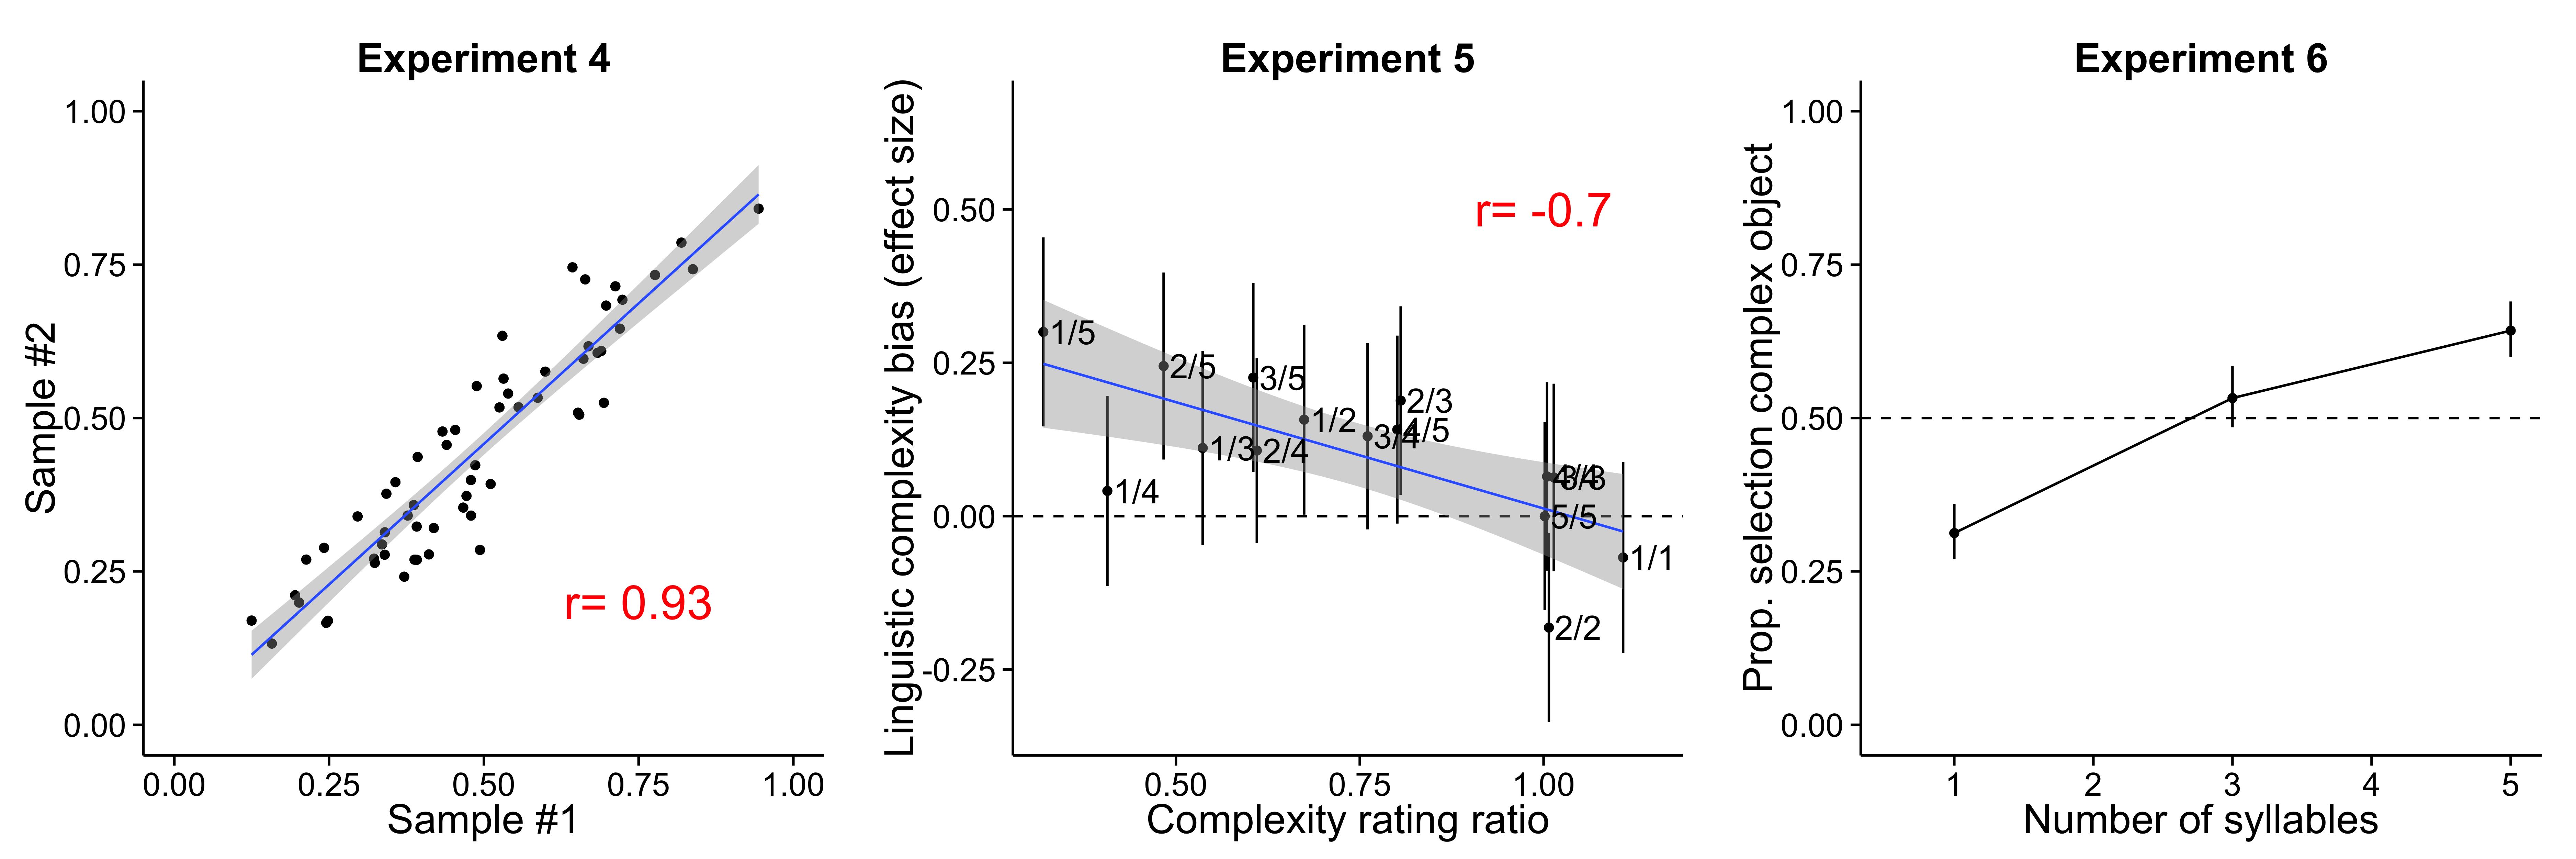
\includegraphics[width=6in]{figs/study2_plots.png}
  \caption{\label{fig:study2_plots} (a) The correlation between the two samples of complexity norms. Each point corresponds to an object ($n = 60$). (b) Effect size (bias to select complex alternative in long vs.\ short word condition) as a function of the complexity rating ratio between the two object alternatives. Each point corresponds to an object condition. Conditions are labeled by the complexity norm quintile of the two alternatives. (c) The proportion of complex object selections as a function of number of syllables. The dashed line reflects chance selection between the simple and complex alternatives. All errors bars reflect 95\% confidence intervals, calculated via non-parametric bootstrapping in 4 and 6, and parametrically in 5.}
 \end{center}
\end{figure}
 Complexity judgments were highly reliable across two independent samples ($r = .93, p < .0001$; $M_1 = .49$, $SD_1 = .18$, $M_2 = .44$, $SD_2 = .18$; mean difference = $.07$). Figure \ref{fig:study2_plots}a shows the relationship between the complexity judgment for each item across the two samples of participants. Figure \ref{fig:realobjs} shows all 60 objects sorted by their mean complexity rating.

\section{Experiment 5: Mapping Task (Novel Real Objects)}
\label{ch2-5}

\subsection{Methods}
\subsubsection{Participants} 1500 participants completed the experiment.
\subsubsection{Stimuli} The linguistic stimuli were identical to Experiment 2. The object stimuli were the 60 naturalistic objects normed in Experiment 2. Five complexity conditions were determined by dividing the objects into quintiles based on the norms.

\subsubsection{Procedure} The procedure was identical to Experiment 2, except for the use of naturalistic rather than artificial geon objects.

\subsection{Results and Discussion}
As with the artificial objects, effect size was negatively correlated with the complexity rating ratio between the referent alternatives ($r = .70, p < .005$; Fig. \ref{fig:study2_plots}b). This suggests that the complexity bias observed with artificial objects extends to more naturalistic objects, consistent with the proposal that a complexity bias is a characteristic of natural language more generally.

The effect size in Experiment 5 is smaller than in Experiment 2, however. This difference may be due to the fact that some of the effect in Experiment 2 was due to task demands associated with the transparent complexity manipulation. Nonetheless, Experiment 5 reveals a complexity bias with naturalistic objects.

\section{Experiment 6: Control Mapping Task (Novel Objects)}
As with the artificial objects, we sought to control for the possibility that the results from the mapping task were due to our particular linguistic items. Thus, we conducted a control experiment analogous to Experiment 3 using randomly concatenated syllables.

\subsection{Methods}
\subsubsection{Participants} 200 participants completed the experiment.
\subsubsection{Stimuli} The objects were 12 objects from the first and fifth quintile of complexity norms. The linguistic stimuli were constructed as in Experiment 3.

\subsubsection{Procedure}
The procedure was identical to Experiment 3, except for the different object stimuli.

\subsection{Results and Discussion}
We fit the same model as in Experiment 3, predicting response value with length using a generalized liner mixed-effect model. A model with random by-participant slopes and intercepts failed to converge, and so the final model included only random by-participant intercepts. Participants were more likely to select an object from the fifth quintile as opposed to the first quintile when the novel word contained more syllables ($\beta = -.35$, $z = -.91$, $p < .0001$; Fig.\ \ref{fig:study2_plots}c). This pattern replicates the complexity bias seen in Experiment 5 with randomly concatenated syllables.

In the present experiment, participants were overall less likely to select the complex object, compared to the same experiment with artificial objects (consider the overall higher level of complex-object judgments in Experiment 5). This finding may be due to the fact that some of the simple artificial objects in Experiment 3 are associated with canonical labels (e.g., the sphere single-geon object may have evoked the label ``ball.''). Perhaps this feature of hte stimuli might have lead participants to appeal to mutual exclusivity in their object selections by selecting an object they do not already have a name for---in this case, the more complex object \cite{markman1988}. Alternatively, the novel artificial objects could be overall less complex than the geon objects. Regardless of this shift, however, the critical finding is that we replicate the complexity bias with random syllables in both Experiments 3 and 6.

\section{Experiment 7: Label Production Task (Novel Objects)}

The previous set of experiments provides evidence for a complexity bias in a comprehension task with novel words. One limitation of this design, however, is that participants may have been influenced by task demands associated with making a forced choice between two contrasting alternatives. In Experiment 7, we sought to minimize these demands by presenting participants with an object and asking them to produce a novel label to refer to it. Consistent with a complexity bias, we find that participants produce longer labels for more complex objects.

\subsection{Methods}
\subsubsection{Participants} Fifty-nine participants completed the experiment.
\subsubsection{Stimuli} The objects were drawn from the set of 60 naturalistic objects used in Experiments 4-6
\subsubsection{Procedure}
In each trial, we presented a single object and asked participants to generate a novel single-word label to refer to it. The instructions read:

\begin{quote}
What do you think this object is called? For example, someone might call it a {\it tupa} or a {\it pakuwugnum}. In the box below, please make up your own name for the object. Your name should only be one word. It should not be a real English word.
\end{quote}
Each participant completed 10 trials---five objects from the bottom and top complexity norm quantiles each. Order of objects was randomized.

\subsection{Results and Discussion}
There were 26 productions (4\%) that included more than one word. These productions were excluded. Length was measured in terms of log number of characters.

Participants produced novel coinages that varied in length (e.g., ``keyo,'' ``plattle,'' ``scrupula,'' ``frillobite''). Critically, productions tended to be longer for the top quartile of objects ($M = 7.13$, $SD = 1.81$ characters) compared to the bottom quartile ($M = 6.60$, $SD = 1.78$ characters). To test the reliability of this difference, we fit a linear mixed-effect model predicting log length in terms of number of characters with complexity norm as a fixed effect. The random effect structure included by-participant intercepts and slopes. There was a reliable effect of complexity norms, suggesting that productions tended to be longer for more complex objects ($\beta = .19$, $t = 4.36$). This experiment provides strong evidence for a productive complexity bias: Even with minimal task demands, participants prefer to use longer words to refer to more complex objects.

\section{Experiments 8a and 8b: Complexity as a Cognitive Construct}
Experiments 1--7 suggest that participants have a productive complexity bias when complexity is operationalized in terms of explicit norms. In Experiment 8, we try to more directly examine the cognitive correlates of conceptual complexity. We reasoned that if complexity is related to a basic cognitive process, we should be able to measure it using an implicit task, not just via explicit ratings.

To measure complexity implicitly, we adopt a measure from the visual processing literature: reaction time. In this literature, the amount of information in a stimulus is argued to be monotonically related to the amount of time needed to respond to that stimulus. \citeA{hyman} demonstrated this using a task in which participants were asked to indicate which light was illuminated from a set of bulbs. Two factors were manipulated to vary the amount of information in each bulb: the number of bulb alternatives and the frequency of each bulb illuminating. They found that the reaction time for responding to an illuminated bulb was linearly related to the amount of information in that bulb. More recently, \citeA{alvarez2004capacity} used a reaction time measure---search rate---to quantify the amount of information in a varied set of visual stimuli. They found that the search rate of a visual stimulus was monotonically related to the memory capacity for that stimulus. Finally, in the domain of sentence processing, reaction time has been directly correlated with measures of surprisal of a word in its linguistic context \cite{demberg2008data,levy2008expectation}. Together, these results suggest that reaction time may be a behavioral correlate of the amount of information, or complexity, of a stimulus.

To collect an implicit measure of complexity for our objects, we measured participants' study time of objects in a memory task. Each participant studied half of the objects in the stimulus set, one at a time, and then made old/new judgments for the entire set. Critically, the study phase was self-paced, such that participants were allowed to study each object for as much time as they wanted. This study time provided an implicit measure of complexity. For both the artificial (Experiment 8a) and naturalistic (Experiment 8b) objects, we found that participants tended to study objects longer when they were rated as more complex.

\subsection{Methods}
\subsubsection{Participants} 750 participants completed the task. 250 participants were tested with artificial objects (Experiment 8a) and 500 were tested with novel real objects (Experiment 8b).
\subsubsection{Stimuli} The study objects were the set of 40 artificial objects (Experiment 8a) and 60 novel real objects (Experiment 8b).

\subsubsection{Procedure} Participants were told they were going to view some objects and their memory of those exact objects would later be tested. In the study phase, participants were presented with half of the full stimulus set one at a time (20 artificial objects and 30 novel real objects) and allowed to click a ``next'' button when they were done studying each object. After the training phase, we presented participants with each object in the full stimulus set (40 artificial objects and 60 novel real objects), and asked ``Have you seen this object before?.'' Participants responded by clicking a ``yes'' or ``no'' button.

\subsection{Results and Discussion }
\subsubsection{Experiment 8a: Artificial objects}
We excluded subjects who performed at or below chance on the memory task (20 or fewer correct out of 40). A response was counted as correct if it was a correct rejection or a hit. This excluded 9 participants (4\%). With these participants excluded, the mean correct was 72\%. Participants were also excluded based on study times. We transformed the time into log space, and excluded responses that were 2 standard deviations above or below the mean. This excluded 4\% of responses (final sample: $M = 2.02$, $SD = 1.37$ {\it s}).

Next, we examined study times for each object in this ($M = 1.89$, $SD = .28$ {\it s}). Study times were highly correlated with the number of geons in each object ($r=.93$, $p<.0001$): objects that contained more geons tended to be studied longer. Study times were also highly correlated with the explicit complexity norms ($r = .89$, $p < .0001$): objects that were rated as more complex tended to be studied longer.

The critical question was whether mean study times for an object were related to the bias to assign a long or short word to that object. To explore this question, we reanalyzed the data from Experiment 2 in terms of study times instead of explicit complexity norms. The ratio of study times for the two object alternatives was correlated with the bias to choose a longer label ($r = .82$, $p < .001$; Fig.\ \ref{fig:study3_plots}a): Relatively longer study times predicted longer labels.

 \begin{figure}
 \begin{center}
  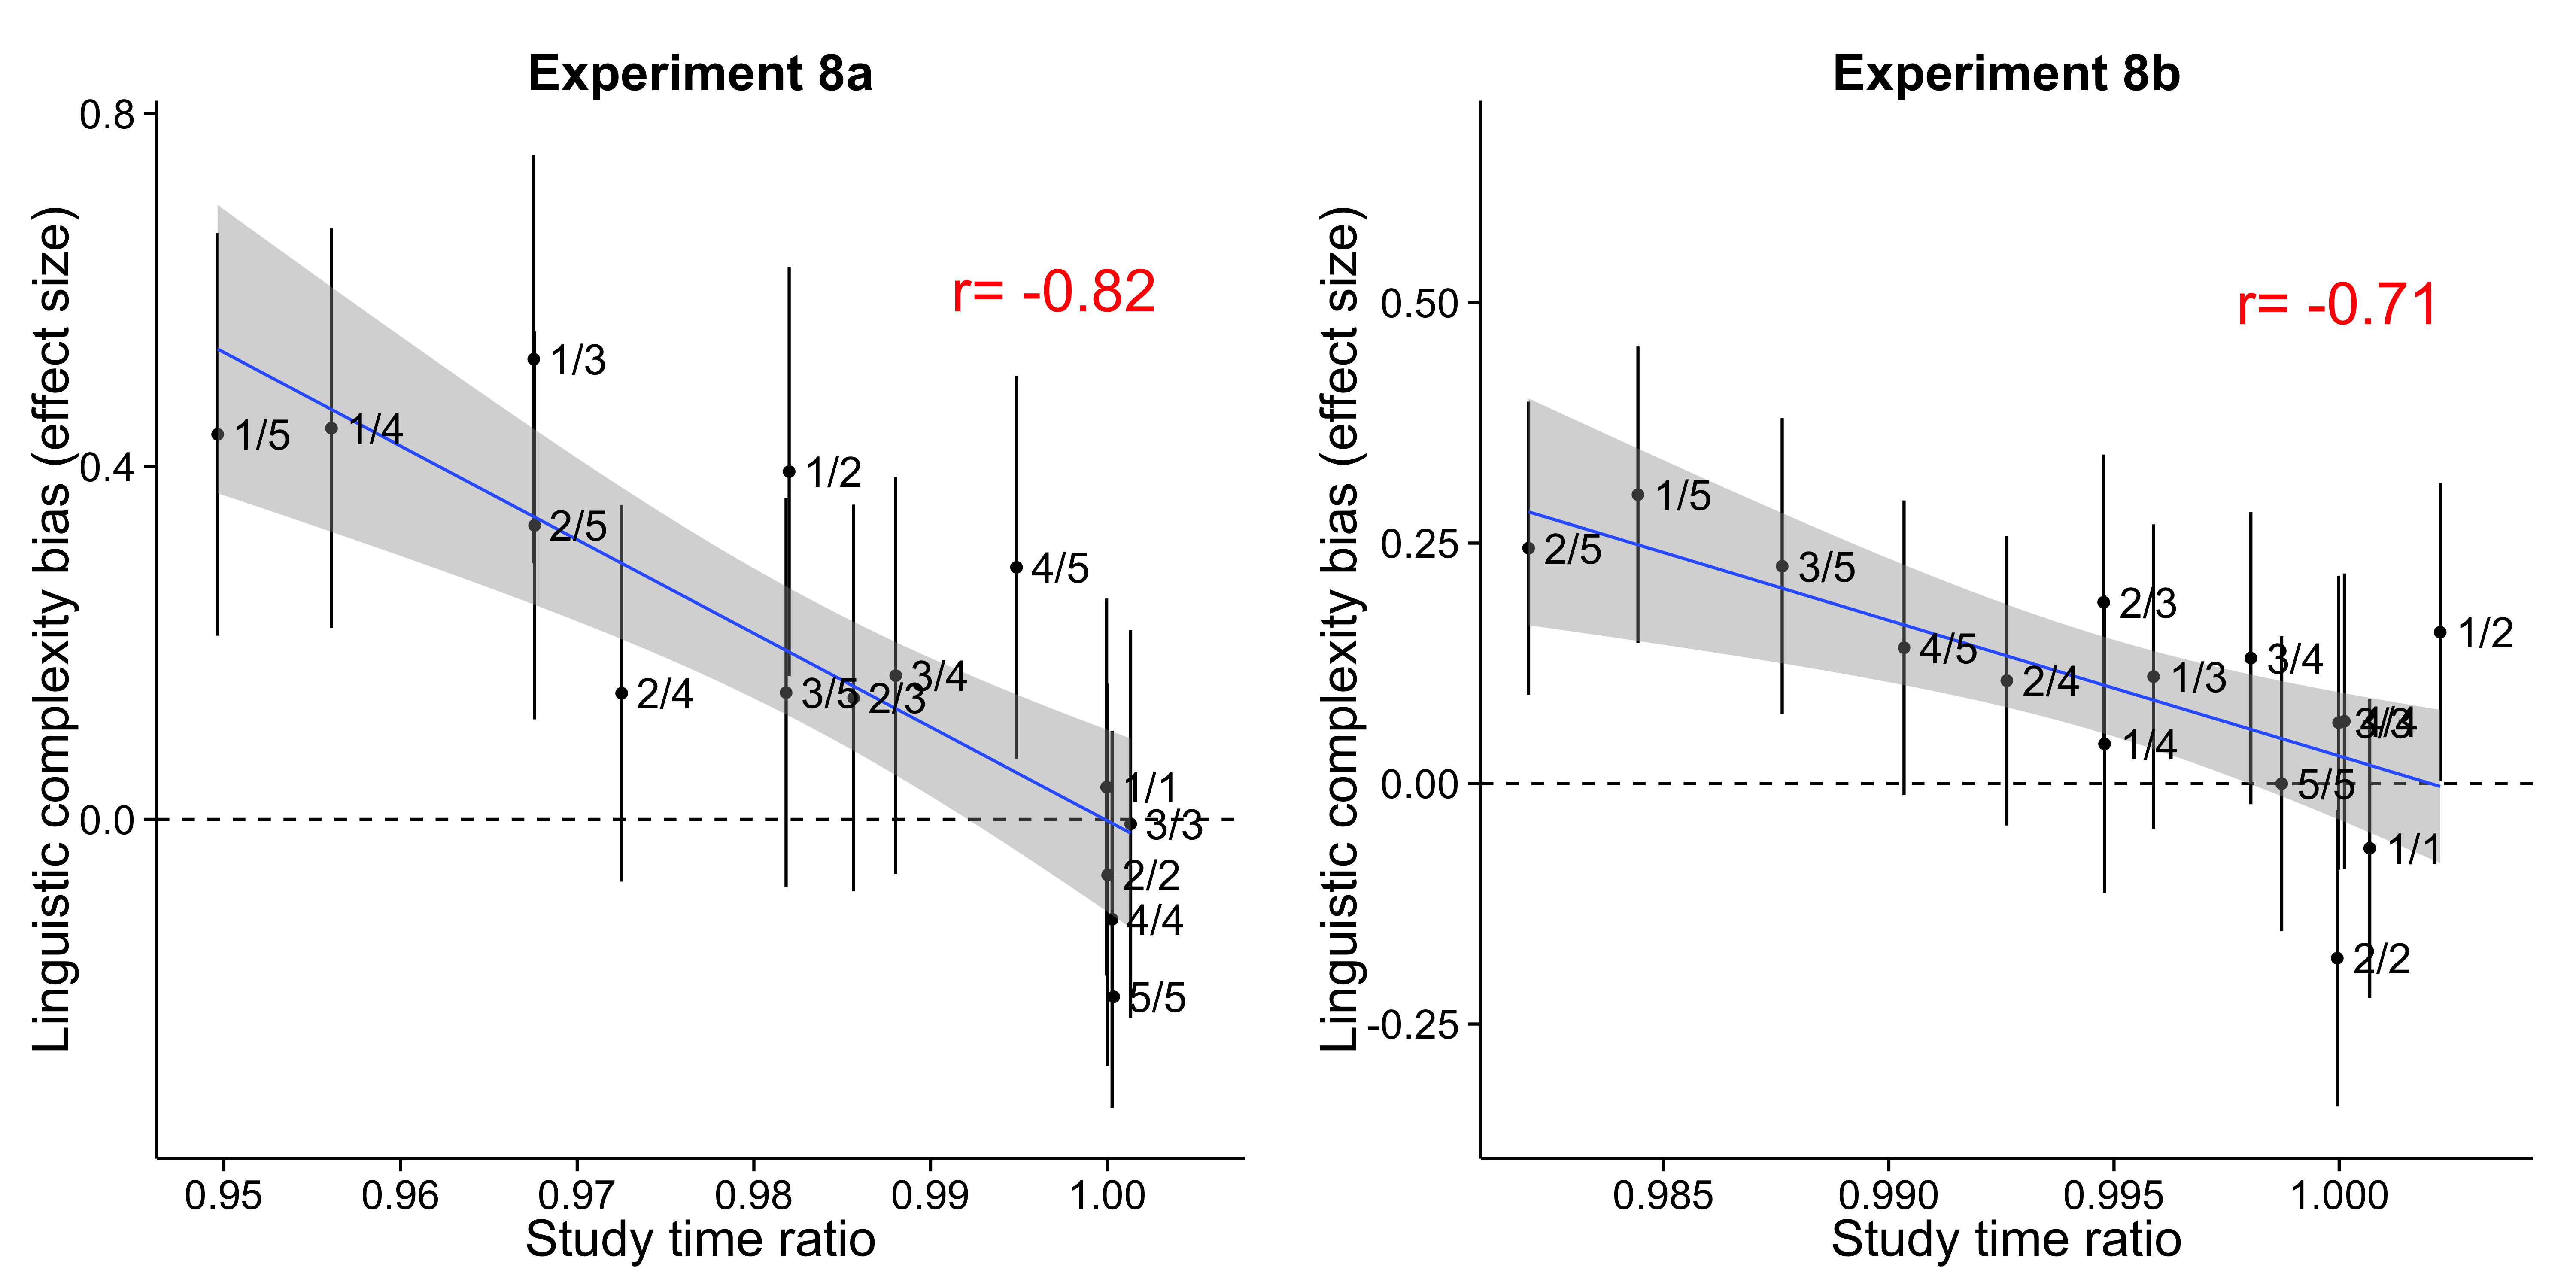
\includegraphics[width=6in]{figs/study3_plots.png}
  \caption{\label{fig:study3_plots} Effect sizes in Experiments 2 and 4 replotted in terms of study times collected in Experiment 8. Objects that are studied relatively longer are more likely to be assigned a longer label, relative to a shorter label. Error bars show 95\% confidence intervals.}
 \end{center}
\end{figure}

\subsubsection{Experiment 8b: Novel real objects}
\label{ch2-8b}
We excluded six (1\%) participants who performed at or below chance on the memory task (30 or fewer correct out of 60). A response was counted as correct if it was a correct rejection or a hit. With these participants excluded, the mean correct was 84\%. Participants were also excluded based on study times, using the same criteria as in Experiment 8a, leading to the exclusion of 4\% of responses (final sample: $M = 2.01$, $SD = 1.45$ {\it s}).

We next examined study times by object ($M = 1.92$, $SD = .18$ {\it s}). Study times were highly correlated with explicit complexity norms for each object. Like for the geons, objects that were rated as more complex were studied longer ($r = .54$, $p < .0001$). This correlation was somewhat smaller than for the geons ($r = .89$), which may be due to the fact that overall variance in study times was smaller for the real objects ($SD = .18$), relative to the geons ($SD = .28$). Critically, by reanalyzing data from Experiment 4 in terms of study times, we find that the ratio of study times for the two objects was correlated with the bias to choose a longer label ($r = .71$, $p < .005$; Fig.\ \ref{fig:study3_plots}b).

Together, these findings suggest that label judgments are supported by basic cognitive processes related to the complexity or information content of a stimulus. More broadly, Experiments 1-8 point to a complexity bias in interpreting novel labels: Words that are longer tend to be associated with meanings that are more complex, as reflected in both explicit and implicit measures.

\section{Experiment 9: Complexity Bias in Natural Language}
\label{ch2-9}

Experiments 1--8 revealed a productive complexity bias in the case of novel words (Hypothesis 1). Next we ask whether this bias extends to natural language (Hypothesis 2). In Experiment 9, we collected explicit complexity judgments on the meaning of 499 English words in a rating procedure similar to Experiments 1 and 4 above. Consistent with a complexity bias, we find that complexity ratings are highly correlated with word length in English: Words with meanings that are rated as more complex tend to be longer.

To measure conceptual complexity in natural language, we adopt a rating scale approach similar to that used in previous work \cite<e.g.,>{wilson1988mrc} to quantify other aspects meaning, like how perceptible a referent is (concreteness) and how much experience speakers tend to have with a referent (familiarity). In this work, participants are presented with a 5- or 7- point Likert scale anchored at both ends of the target dimension and asked to make an explicit judgment about a word's meaning. A limitation of this approach is that it requires that all participants conceptualize the dimension of interest in a similar way. Nonetheless, previous work has shown these measures to be reliable and so we adopt them here to quantify conceptual complexity.

\subsection{Methods}
\subsubsection{Participants} 246 participants completed the norming procedure.
\subsubsection{Stimuli}
We selected 499 English words from the MRC Psycholinguistic Database \cite{wilson1988mrc} that were broadly distributed in their length and were relatively high frequency. This database includes norms for three other psycholinguistic variables: concreteness, familiarity, and imageability. This selection of items allowed us to compare our complexity norms to previously measured psycholinguistic variables that are intuitively related to complexity.

\subsubsection{Procedure}
Participants were first presented with instructions describing the norming task:
\begin{quote}
In this experiment, you will be asked to decide how complex the meaning of a word is. A word's meaning is simple if it is easy to understand and has few parts. An example of a simple meaning is ``brick.'' A word's meaning is complex if it is difficult to understand and has many parts. An example of a more complex meaning is ``engine.''
\end{quote}
For each word, we then asked ``How complex is the meaning of this word?,'' and participants indicated their response on a 7-pt Likert scale anchored at ``simple'' and ``complex.'' The first two words were always ``ball'' and ``motherboard'' to anchor participants on the scale. Each participant rated a sample of 30 words English words. After the 17th word, participants were asked to complete a simple math problem to ensure they were engaged in the task.

\subsection{Results and Discussion}

We first examined word length in our samples of words, using three different metrics of word length: phonemes, syllables, and morphemes. Measures of phonemes and syllables were taken from the MRC corpus \cite{wilson1988mrc} and measures of morphemes were taken from CELEX2 database \cite{baayen1995celex2}. All three metrics were highly correlated with each other (phonemes and syllables: $r = .89$; phonemes and morphemes: $r = .65$; morphemes and syllables: $r = .67$). All three metrics were also highly correlated with number of characters, the unit of length with use in the cross-linguistic corpus analysis below (phonemes: $r = .92$; morphemes: $r = .69$; syllables: $r = .87$).

Given these measures of word length, we next considered how length related to judgments of meaning complexity. We excluded 6 participants (2\%) who missed the math problem, our attentional check. Critically, we found that complexity ratings ($M = 3.36$, $SD = 1.14$) were positively correlated with word length, measured in phonemes, syllables, and morphemes ($r_{phonemes} = .67$, $r_{syllables} = .63$, $r_{morphemes} = .43$, all $p$s $< .0001$, Fig. \ref{fig:study4a_plot}).\footnote{All norms can be found here: \url{https://github.com/mllewis/RC/blob/master/data/norms/}. } This relationship held for the subset of only open class words ($n = 438$; $r_{phonemes} = .65$, $r_{syllables} = .63$, $r_{morphemes} = .42$, all $p$s $< .0001$). Word class was coded by the authors.

 \begin{figure}
 \begin{center}
  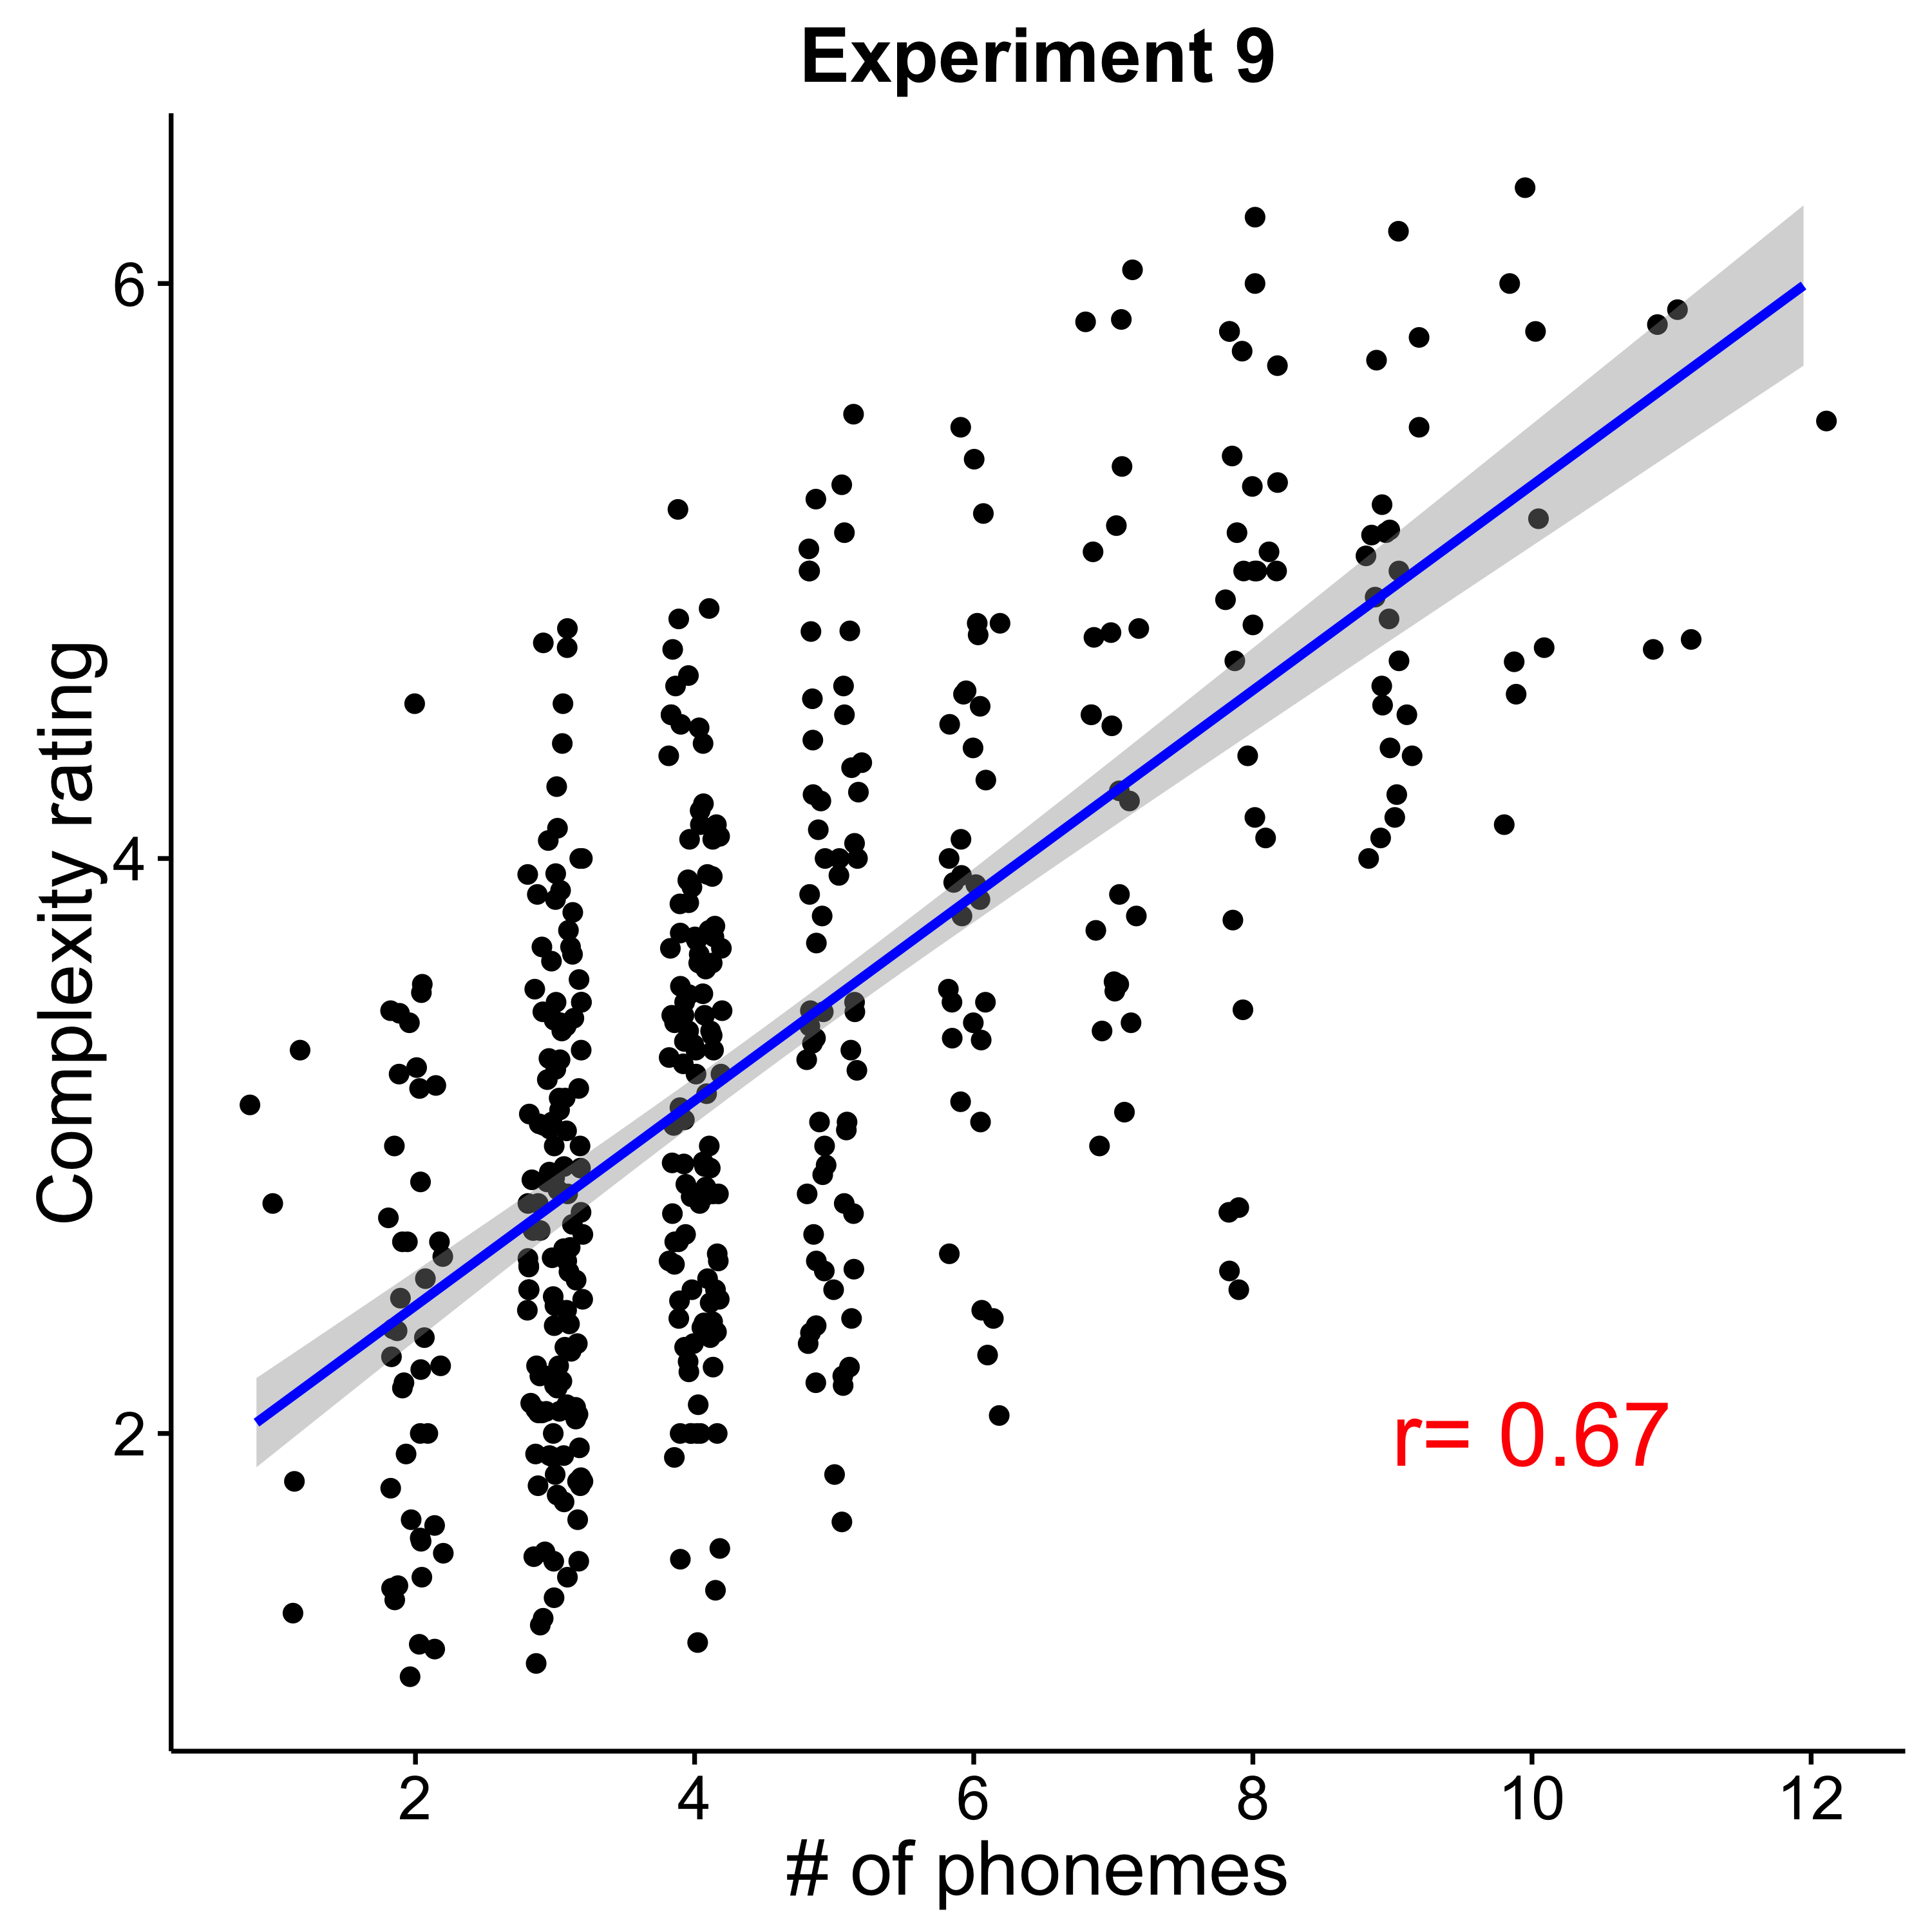
\includegraphics[width=3in]{figs/study4a_plot.png}
  \caption{\label{fig:study4a_plot} Complexity norms collected in Experiment 9 as a function of word length in terms of number of phonemes. Words rated as more complex tend to be longer. Error bars show bootstrapped 95\% confidence intervals.}
 \end{center}
\end{figure}

This result points to a relationship between conceptual complexity and word length, but to interpret this relationship, it is important to also control for other known correlates of word length and complexity. Linguistic predictability is highly correlated with word length, operationalized via simple frequency \cite{zipf1936} or using a language model \cite{piantadosi2011b}. We estimated word frequency from a corpus of transcripts of American English movies \cite<Subtlex-us database; >{brysbaert2009moving}. Importantly, the regularity we describe---a relationship between conceptual complexity and word length---holds even when controlling for frequency. In English, the correlation was only slightly reduced when controlling for log frequency ($r = .57$, $p < .0001$).

We also looked at the relationship between length and complexity controlling for the average predictability of a word in a linguistic context (its surprisal). As discussed in the Introduction, recent work suggests that surprisal may be stronger correlate of length than frequency \cite{piantadosi2011a}. We included bigram surprisal values for our set of 499 words calculated from the British National Corpus \cite{clear1993british}.\footnote{We thank Steve Piantadosi for sharing this data with us.} Surprisal was correlated with complexity ($r = .29$, $p < .0001$), but the correlation between length in phonemes and complexity remained reliable after partialing out surprisal ($r = .62$, $p < .0001$). In an additive linear model predicting word length (phonemes) with complexity, frequency, and surprisal, complexity and surprisal were reliable predictors of length ($\beta = 1.11$, $t = 17.22$, $p < .0001$; $\beta = .66$, $t = 2.3$, $p = .02$), but frequency was not ($\beta = .04$, $t = .39$, $p =. 70$).

Complexity is reliably correlated with concreteness, familiarity, and imageability (concreteness: $r = -.27$; familiarity: $r = -.43$; imageability: $r = -.21$). Nonetheless, the relationship between word length and complexity remained reliable controlling for these factors. We created an additive linear model predicting word length in terms of phonemes with complexity, controlling for concreteness, imageability, familiarity, and frequency. Model parameters are presented in Table~\ref{exp9model}. This pattern held for the other two metrics of word length (morphemes and syllables).

% latex table generated in R 3.1.0 by xtable 1.7-4 package
% Thu Jul 16 17:07:52 2015
\begin{table}[t]
\centering
\begin{tabular}{rrrrr}
 \hline
 & Estimate & Std. Error & $t$-value & $p$ \\
 \hline
(Intercept) & 7.5020 & 0.2061 & 36.40 & $<$.001 \\
 complexity & 0.2429 & 0.0116 & 20.86 & $<$.001\\
  concreteness & -0.0033 & 0.0004 & -9.16 & $<$.001 \\
 imageability & -0.0003 & 0.0004 & -0.81 & 0.42 \\
  familiarity & 0.0024 & 0.0005 & 4.80 & $<$.001 \\
 log frequency & -1.1556 & 0.0332 & -34.80 & $<$.001 \\
  \hline
\end{tabular}
\caption{Model parameters for linear regression predicting word length in terms of semantic variables and word frequency.}
\label{exp9model}
\end{table}


This result extends beyond the findings of previous work on markedness. Although this difference in the complexity of morphological structure could in principle contribute to conceptual complexity judgments, it does not explain the pattern in our data. The correlations we observed hold for words with no obvious derivational morphology \cite<CELEX2 monomorphemes;>[$n = 387$; $r_{phonemes} = .53$, $r_{syllables} = .47$, all $p$s $< .0001$]{baayen1995celex2}.

Finally, languages also show phonological iconicity effects, such that semantic features \cite{maurer2006shape} and even particular form classes \cite{farmer2006phonological} are marked by particular sound patterns. However, the type of iconicity explored here is broader---a systematic relationship between abstract measures of complexity and amount of verbal or orthographic effort. Specific iconic hypotheses that posit a parallel between an object's parts and the number of phonemes, morphemes, or syllables in its label do not account for the patterns in the English lexicon: The length-complexity correlation holds even more strongly for words that are not object labels ($n=336$; $r_{phonemes}= .73$, $p<.001$), compared to object labels ($n=163$; $r_{phonemes}= .44$,$p<.001$), whose part structure is presumably much less obvious. If true, this suggests the effect sizes in Experiments 1-8 may be conservative estimates of the bias since all referents in these experiments were concrete objects.

While correlational nature of this study makes inferences about causality tentative---complex meanings may be assigned longer words, or words that are longer may be rated as more complex---this study nonetheless points to a robust relationship between word length and conceptual complexity in English.

\section{Study 10: Cross-Linguistic Corpus Analysis}

If the complexity bias relies on a universal cognitive process, it should generalize to lexicons beyond English. We explored this prediction in 79 additional languages though a corpus analysis, and found a complexity bias in every language we examined.

\subsection{Methods and Results}
We translated all 499 words from Experiment 9 into 79 languages using Google translate (retrieved March 2014). The set of languages was the full set available in Google translate. Words that were translated as English words were removed from the data set. We also removed words that were translated into a script that was different from the target language (e.g., an English word listed for Japanese).

Native speakers evaluated the accuracy of these translations for 12 of the 79 languages. Native speakers were told to look at the translations provided by Google, and in cases where the translation was bad or not given, provide a ``better translation.'' Translations were not marked as inaccurate if the translation was missing. Across the 12 languages, there was .92 native speaker agreement with the Google translations across all 499 words.

To test for a complex bias, we calculated the length of each word in each of the 79 languages using number of unicode characters as our unit of length (to allow comparison between languages for which no phonetic dictionary was available). For each language, we calculated the correlation between word length in terms of number of characters and mean complexity rating. All 79 languages showed a positive correlation between length and complexity ratings. The grand mean correlation across languages was .34 ($r$ = .37, for checked languages only).

This relationship between word length and complexity remained reliable in a number of control analyses. There was a reliable correlation between length and complexity for the subset of English monomorphic words (grand mean $r$ = .23) and open class words (grand mean $r$ = .30). It also held partialling out frequency (grand mean $r$ = .22).

Finally, it is possible that the cross-linguistic regularity is due primarily to a genetic relationship between languages or language contact \cite{jaeger2011mixed}. Such a finding would suggest that the bias may be an idiosyncratic property of a few languages, rather than a broad generalization of human languages. To test this possibility, we used data from the  World Atlas of Language Structures database \cite<WALS;>{haspelmath2005world}. We included language family as a control for genetic relationships and native country as a control for language contact. Data was available for 68 of our 80 languages in this dataset. Within these languages, there were 16 language families and 49 countries represented.

We constructed a mixed effect model predicting word length in terms of number of characters with complexity ratings and log frequency as fixed effects. The random-effect structure included language family as both random slopes and intercepts.\footnote{The model specification was as follows: \texttt{word length $\sim$ complexity + log frequency + (1 + complexity + log frequency~\textbar~language family) +  (1 + complexity + log frequency~\textbar~native country)}. This structure was the maximal random effect structure that allowed the model to converge.}  The model showed a reliable effect of complexity on length ($\beta = .70$, $t = 3.59$), suggesting that the complexity bias is present in a wide range of languages.

 \begin{figure}
 \begin{center}
  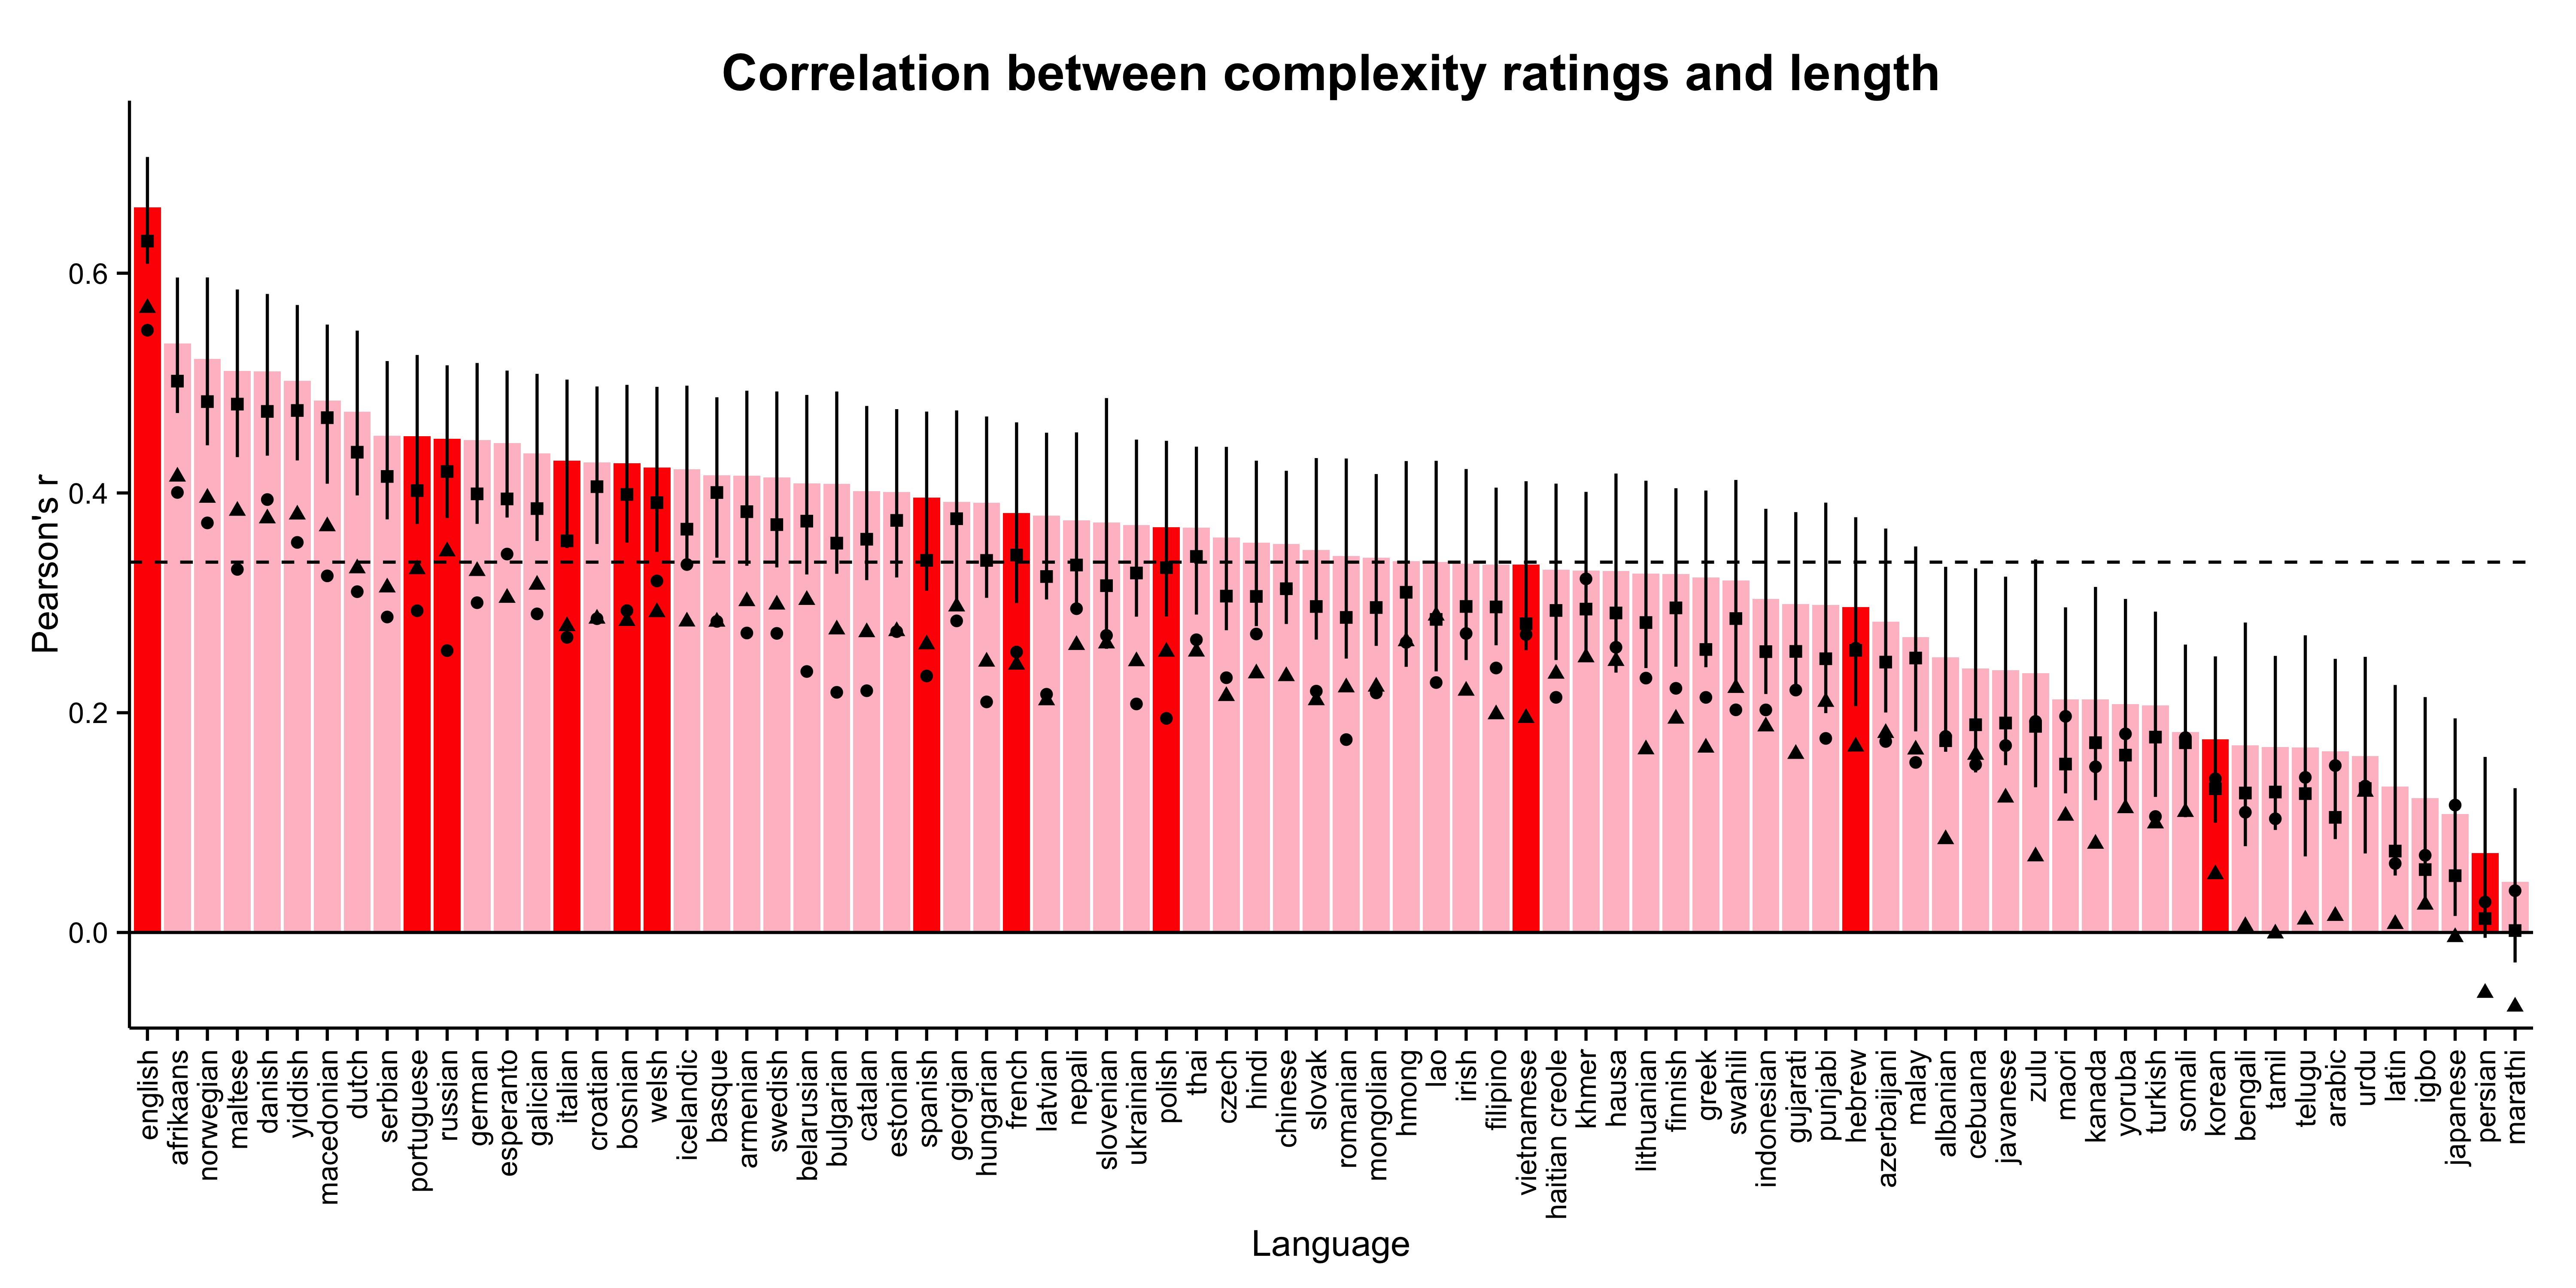
\includegraphics[width=6.3in]{figs/xling_plot.png}
  \caption{\label{fig:study4a_plasd} Correlation coefficient (Pearson's $r$) between length in unicode characters and conceptual complexity rating (obtained in Experiment 9). Dark red bars indicate languages for which translations were checked by native speakers; all other bars show translations obtained via Google Translate. The dashed line indicates the grand mean correlation across languages. Triangles indicate the correlation between complexity and length, partialling out log spoken frequency in English. Circles indicate the correlation between complexity and length for the subset of words that are monomorphemic in English. Squares indicate the correlation between complexity and length for the subset of open class words. Error bars show 95\% confidence intervals obtained via non-parametric bootstrap. }
 \end{center}
\end{figure}


\subsection{Discussion}

This corpus analysis suggests that the complexity bias found in natural language (Experiment 9) generalizes to a broad range of other languages. A notable result from these analyses is that English appears to have the largest complexity bias of the languages examined. One possible explanation is that, because our complexity norms were elicited for English words, our measure of conceptual complexity was most accurate for English words, and thus the complexity bias was largest for English. If true, then the cross-linguistic estimates of complexity bias obtained in the present analyses would be conservative estimates of a larger bias.


\section{General Discussion}

We began with two observations---the presence of many pragmatic equilibria reflected in the structure of the lexicon, and the fact that several theories of pragmatics predict a tradeoff between length and complexity. The goal of our work was to explore whether a tradeoff between length and complexity is present in words---namely, a bias for longer words to refer to more conceptually more complex meanings. We explored this bias at two timescales. At the pragmatic timescale, we asked whether participants would be biased to assign a relatively long novel word to a conceptually more complex referent (Hypothesis 1). At the language evolution timescale, we asked whether languages tended to encoded conceptually more complex meanings with longer forms (Hypothesis 2). We found support for both hypotheses.

Experiments 1--7 suggest that when conceptual complexity is operationalized via visual complexity, participants are biased to assign novel words to more complex referents. This pattern holds true for both artificial objects where visual complexity was directly manipulated, as well as for naturalistic objects where we measured visual complexity and analyzed it correlationally. We also found this pattern across both comprehension and production tasks, suggesting this bias was not merely the result of task demands. Experiment 8 reveals that visual complexity is highly correlated with an implicit measure---study time---and this measure predicts the bias to assign an object a long or a short word. Finally, Experiment 9 suggests that explicit measures of conceptual complexity in English are highly correlated with word length in English, and the corpus analysis reveals a correlation between English complexity norms and word lengths in a diverse set of languages.

These studies reveal a regularity in language that appears to be productive and true cross-linguistically. The observed bias is highly general, both in terms of the unit of length (phonemes, morphemes, and syllables) as well as the characterization of semantics. This work contributes an important extension to the previous work on markedness. Previous work on markedness described relationships between conceptual features and word length that were post-hoc and domain specific. Our work suggests that conceptual complexity may be a unifying framework for thinking about variability in conceptual space across semantic domains. In our work here, we begin to directly address the cognitive construct underlying conceptual complexity by revealing a strong relationship between explicit measures of complexity and the implicit measure of reaction time.

While the broad nature of the regularity we describe is a strength, our work here leaves a number of open questions. Additional research needs to be done to better understand what conceptual complexity is and what constructs our measures here describe. Our reaction time results suggest that, whatever conceptual complexity is, it is related to basic cognitive processes. But our work does not provide any insight into what the conceptual primitives are such that some meanings are more conceptually complex than others. We turn to this issue in Chapter 3.

A second limitation of our work is that we are not able to provide an account of why word lengths can change over time for the same meaning (e.g., ``television'' becomes ``TV'' or ``cellular phone'' becomes ``cell''). The answer to this question may be related to the question of conceptual complexity. One possibility is that the conceptual complexity of a word's meaning may reduce over time, and language reflects this change by shortening the length of the word. Another possibility is that this reduction is the result of another pressure on language change: word frequency. Under this hypothesis, as a word become more frequent, it becomes shorter \cite{zipf1936}, and this pressure is independent of the complexity bias. So perhaps such shortenings are unrelated to the phenomenon we describe here.

Finally, our interpretation of this work is limited by the fact that all participants were speakers of English. A complexity bias could in principle be idiosyncratic to English. The results from our experiments with novel words would then be the product of speakers merely generalizing from their native language. Relatedly, the fact that all participants spoke English is also a limitation for our interpretation of the cross-linguistic corpus analysis. Because our complexity norms were elicited for English words from English speakers, the ratings are likely imperfect measures of conceptual complexity for words translated into other languages. Thus, it is difficult to know whether variability in the magnitude of the complexity bias cross-linguistically is due to true underlying differences in the bias, or merely a difference in the fidelity of the complexity ratings cross-linguistically. Speaking against this limitation, however, the presence of a complexity bias across all 80 languages that we examined suggests that the bias is likely to hold cross-linguistically in experimental work as well. If anything, the cross-linguistic mean bias is likely larger than our current estimates in the corpus study, because of the mismatch in complexity judgments between English speakers and speakers of other languages.

The motivating framework for the present work was the notion of interacting dynamics at multiple timescales. Our work suggests that a complexity bias is present in both individual speakers---the pragmatic timescale (Hypothesis 1)---and in the structure of the lexicon---the language evolution timescale (Hypothesis 2). While the existing data do not speak directly to a causal relationship between these two hypotheses, a casual interpretation is both parsimonious and consistent with work in other domains of linguistic structure, reviewed in the Introduction. A causal account would suggest that the trade off between listener and hearer pressures leads to a complexity bias at the pragmatic timescale and, over time, these pressures lead to the same regularity emerging in the lexicon over the language change timescale. Our data are not able to speak to the processes underlying participants' judgments---these judgments need not reflect in-the-moment pragmatic inference; they could also be the result of an iconic mapping between effort and meaning, or a lower-level statistical regularity extracted through extensive experience with a language. Regardless of the cognitive instantiation of this inference, the result is lexicons that reflect Horn's principle.

\nocite{saussure}


%!TEX root = ../dissertation.tex

\chapter{What is conceptual complexity?}
\label{chapter:complexity}

The studies in Chapter 2 provide robust evidence for a regularity between word length and a dimension of word meaning, complexity. In these studies, we operationalized the notion of complexity by manipulating the visual complexity of objects in terms of number of component parts. We found that the number of parts  positively correlated with participants' study time in a memory task, providing additional evidence that the stimulus complexity was psychologically relevant. Furthermore, we found that the notion of conceptual complexity extended beyond the visual domain to abstract word meanings in natural language. This finding points to a theory of conceptual complexity that is more general than simply the number of visual parts associated with an object.  Notably, however, this work leaves open the important question of what exactly this theory is---what makes one meaning more conceptually complex than another? Here we try to more directly address this question. 

To formalize the notion of complexity, we adopt an information theoretic approach \cite{shannon1948}. The central idea of Information Theory is that, within a communication channel, each meaning $m$ is communicated with probability $p$, such that the amount information conveyed by each occurrence of $m$ is $-log(p)$. Critically, if it is assumed that the overall length of the code in the communication channel is minimized, then meanings should be assigned to codes in a particular way: Less probable meanings should be assigned to longer codes. By making these assumptions, we establish a fundamental link between the amount of information in a code, its probability of occurrence and its length. In our work here, we appeal to this framework to derive a metric of complexity: More complex codes are longer, less probable, and contain more information.\footnote{This relationship is reflected in the idea of minimum description length proposed by Kolmogorov and others: In a maximally compressed code, more complex codes are longer.} 

Information Theory thus provides a  starting point for evaluating the complexity of a concept by providing a quantitative measure. But, an important property of this theory is that the metric of complexity depends on the representational framework. In other words, what counts as ``one unit" of code in the  channel depends on the representational system that is assumed. This representational agnosticism implies that a meaning that is relatively more complex in one representational framework may relatively less complex in another, or that  complexity in one representational framework may be entirely unrelated to conceptual complexity.

In the case of concepts, it is not a priori obvious what representational framework is most useful in describing their psychological status; what the ``communication channel" of concepts is. The most intuitive is perhaps the Classical View of concepts \cite{laurence1999concepts}, where the units of  representation are primitives and a language for combining them. To illustrate, consider the geon stimuli from Chapter 2:  If we assume that a ``unit" is equivalent to a geon,  then an object composed of a sphere and cone has a conceptual complexity of two, and an object composed of only a sphere, has a conceptual complexity of one. This is the representational framework that is most similar to the approach in Chapter 2. 

Importantly, however, the literature on concepts and categories has explored a range of alternatives to the Classical View \cite{laurence1999concepts}, which we consider in this chapter. In particular,  we consider how the following two views may be related to conceptual complexity:
\begin{quote}
	(1) {\it Classical View}: Concepts are represented as a structured set of primitives.\\
	(2) {\it Statistical View}: Concepts are represented as a set of individual exemplars (Exemplar Theory), or as summary descriptions of exemplars (Prototype Theory).
\end{quote}
We consider each of these views in the broadest form, abstracting away from the many variants within each theory. We then apply Information Theory to each view of concepts and ask what would make one concept more complex than another, assuming the representational framework of that theory. Briefly, for the Classical View, a more complex concept is one with a longer description length. For the Statistical View, a more complex concept is one with more stored exemplars (Exemplar Theory), or with more uncertainty (Prototype Theory). We return to these predictions in more detail below.

We see our goal as not  to distinguish between these  views , nor even that they are incompatible with each other \cite<e.g.,>{murphy2015there,briscoe2011conceptual}. Rather, we consider each of these views as paradigms, in a Kuhnian sense, and ask whether these frameworks can inform our understanding of conceptual complexity when considered in the context of Information Theory. Our approach will be to observe variability in the complexity of meanings as defined within a particular theory of concepts, and ask whether this variability is related to the length of the word that meaning is mapped to. Evidence that a manipulation of conceptual complexity is related to word length would shed light on the underlying construct of conceptual complexity.  

In what follows, we review previous work related to each broad view of concepts---Classical and Statistical---followed by  a series of empirical studies testing  predictions of each view. In total, we conduct seven studies exploring various predictions these theories (see Table~\ref{tab:complexity_pred_summary_table} for summary of our studies). We conclude with a brief summary of our results. 


\bgroup
\def\arraystretch{1.5}% 

\begin{table}[t]
%\footnotesize
\centering
\begin{tabular}{l l l l l }
 \toprule
 \textbf{View} &  \textbf{\begin{tabular}[c]{@{}l@{}}Relevant\\Dimension\end{tabular}} & \textbf{Prediction}& \textbf{\begin{tabular}[c]{@{}l@{}}Relevant\\Studies\end{tabular}} \\
 \toprule
Classical  & \# of primitives & \multicolumn{1}{p{5cm}}{Concepts with longer definitions (and thus more primitives) will be more complex.} & Studies 1-4 \\
Statistical: Exemplar   &  \# of exemplars & \multicolumn{1}{p{5cm}}{Concepts with more  exemplars will be more complex.} & Studies 5-6  \\
Statistical: Exemplar  & Variability of exemplars &\multicolumn{1}{p{5cm}}{Concepts with more variable exemplars will be more complex.} & Study 7 \\
Statistical: Prototype  & \# of exemplars & \multicolumn{1}{p{5cm}}{Concepts with fewer exemplars will have more uncertainty, and thus be more complex.} & Studies 5-6     \\
Statistical: Prototype  & Variability of exemplars &\multicolumn{1}{p{5cm}}{ Concepts with more variable exemplars will have more uncertainty, and thus be more complex.} & Study 7 \\

 \bottomrule
\end{tabular}
\caption{Summary of studies.}
\label{tab:complexity_pred_summary_table}
\end{table}
\egroup

\section{Classical View}
A concept in the Classical View is defined by a rule, or definition, composed of a structured set of conceptual primitives. These definitions are typically considered deterministic of category membership, but more recent work has considered this theory in a probabilistic framework \cite{goodman2008rational}.

This theory has been productively instantiated with Boolean concepts and first-order logic \cite{shepard1961learning,feldman2000minimization,goodman2008rational}.  In this  framework, there are a set of primitives concepts, or predicates, that are represented by binary features, and a syntax for combining them given by first order logic.  For example, consider the concept if \textsc{mother}: If \textsc{female} and \textsc{has\_child} were primitives in the representational language, then  \textsc{mother} would denote the set of people where both primitives were true. 

The information theoretic measure of complexity falls straight-forwardly out of this formulation: Concepts defined by more primitives are more complex \cite{shepard1961learning,feldman2000minimization,goodman2008rational}. In the  above example, then, the complexity of the concept  \textsc{mother} would be two. Consistent with this proposal, there is evidence to suggest that the difficulty of acquiring a concept scales with its conceptual complexity: Concepts that are more difficult to learn tend to have longer definitions\cite{shepard1961learning,feldman2000minimization}.

An important issue for this theory of concepts is identifying a general set of conceptual primitives. Although this task might rank among the deepest challenges for cognitive science, some work has attempted this task. A body of research has sought to understand the innate conceptual primitives in young children (``core knowledge''; Kinzler \& Spelke, 2007). \nocite{kinzler2007core} The proposed set of concepts in this work, however, is restricted to those present only  in early development (e.g., ``agent"), and is therefore not suitable for the broad scope of our current project.  Wierzbicka and colleagues (1996) have also  sought  to identify conceptual primitives, but with a more general focus.  \nocite{wierzbicka1996semantics} This work compares lexical systems across languages  to identify common primitives. The hypothesis is that there exists universal and innate semantic primitives which are the building blocks of meaning in human language. Under this view, all meanings can be derived from a set of numerable semantic primitives and a syntax for combining them.

A related issue is whether the set of primitive concepts  changes over time: Might the conceptual complexity of a concept reduce with experience? That is, might a concept that is initially complex reduce in  complexity, such that it itself becomes an atomic unit in other concepts? This possibility is intriguing, but it remains an open question what sort of experience might lead to a reduction in complexity. One possibility is that the very act of labeling a concept reduces the complexity of a concept\cite{bruner1956austin}. This proposal is consistent with a large body of literature suggesting advantages in concept learning for labeled as opposed to unlabeled categories \cite<e.g.>{balaban1997,lupyan2007,sloutsky2001}. 

However, there is reason to think that other aspects of experience might affect the conceptual complexity of concepts since the length of words can change over time. For example, the word ``telephone" has become more typically ``phone" in standard usage. This type of  diachronic reduction in word length may be due to factors  unrelated to conceptual complexity (e.g.\ frequency of usage), but it might also reflect a decrease in conceptual complexity due to experience, beyond simply tokening the concept. Our work here does not directly address the character of the underlying  primitives, nor whether they are universal or innate or change over time. Rather, it assumes only that such units exist for a speaker and that lexical meanings can vary in the number of their compositional primitives. 

Motivated by the Classical View of concepts, Studies 1-4  explore whether the definition length of a concept  is related to the length of the label denoting that concept. In these studies, we assume that words denote conceptual units, such that concepts associated with longer linguistic definitions are  more complex. We find some evidence in support of this hypothesis.


%``length of the shortest Boolean formula logically equivalent to the concept"

%- Evidence consistent with that: Feldman (Boolean) - learning difficult

%- Issue: where do primitives come from? Might be related to experience. If we new what they were


%\cite{laurence1999concepts,anaki2009familiarity,feldman2016simplicity,goodman2008rational,haskell2011linguistic,lupyan2008conceptual,feldman2000minimization}

%Psychological metrics of complexity - trasnfer vs. recognition. 

%If, however, we assume a different representational framework, we might code this same object with a single conceptual primitive, ``ice cream cone."

\subsubsection{Experiment 1: Descriptions of objects}
In Chapter 2, we presented participants with novel, real objects and measured their complexity through explicit judgements (Exp.\ 4; pg.\ \pageref{ch2-4}) and study time (Exp.\ 8b; pg.\ \pageref{ch2-8b}). Both of these measures showed variability, suggesting that these objects differed in their complexity. 
In Experiment 1, we consider this result in the context of the Classical View of concepts. The Classical View suggests that these objects differ in complexity because they are composed of different number of conceptual primitives, with more complex objects containing more primitives that simpler objects. We reasoned that, if true, these primitives should be reflected in participants linguistic descriptions of the objects. In particular, we predicted that objects rated as more complex and studied longer in Exp.\ 4 and 8b should also be described with longer descriptions. We test this prediction here by asking participants to produce written linguistic description of the objects.


\subsection{Methods}
\subsubsection{Participants} 
In this and all subsequent experiments, participants were recruited on Amazon Mechanical Turk and received US \$0.15-0.50 for their participation, depending on the length of the task. 60 participants completed this first experiment.
\subsubsection{Stimuli} 
We used the same set of 60 novel real objects as in Chapter 2 (Fig. \ref{fig:realobjs}; pg.\ \pageref{fig:realobjs}).

\subsubsection{Procedure}
On each trial, we presented a single object and following instructions:  ``Look at the object below. Imagine you just received this object as a gift. Describe what the object looks like to a friend." Participants then entered their description in a text box below the object.

Each participant described 10 objects in total. Five objects were from the top quantile (high complexity) and 5 objects were from the bottom quantile (low complexity). Order of objects was randomized across trials.

\subsection{Results and Discussion}


\begin{table}[t!]
\centering

\begin{tabular}{ll}
\toprule
\multirow{6}{*}{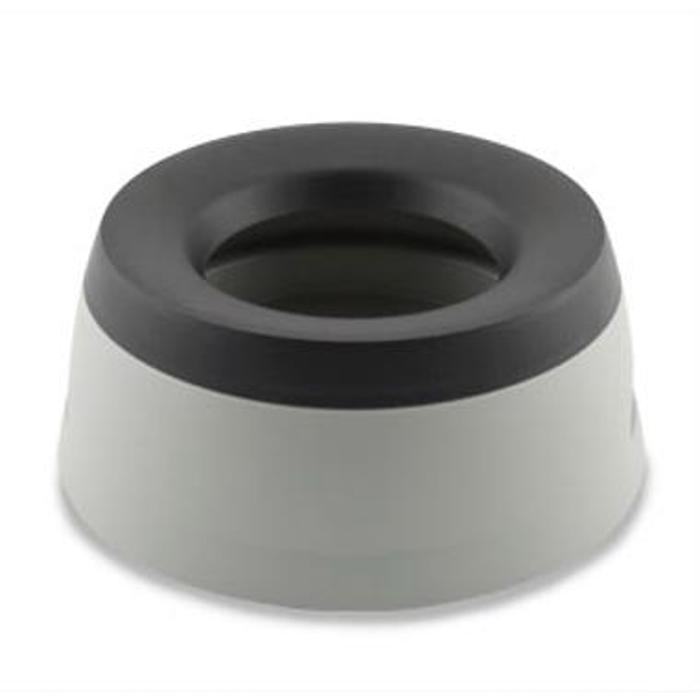
\includegraphics[width=2cm]{figs/obj_29_p2.jpg}} & \textbf{Low-complexity object}                \\
\toprule
                   & ``cup holder"                                   \\
                   & ``it is a bowl with a black portion on top"      \\
                   & ``football kicker's stand"                      \\
                   & ``a hole type thing"                              \\
                   & ``it looks like an ash tray, but a bit shallow" \\
                   & ``looks like a dog bowl" \\
 \bottomrule
~ & ~ \\
  \toprule
\multirow{6}{*}{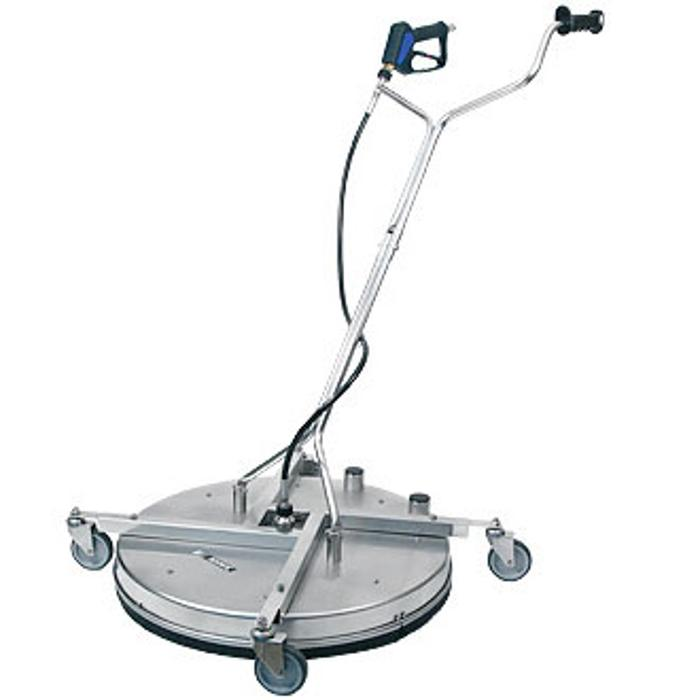
\includegraphics[width=1.8cm]{figs/obj_27_p2.jpg}} & \textbf{High-complexity object}               \\
\toprule
                   & ``a robotic carpet shampooer"                                   \\
                   & \multicolumn{1}{p{12cm}}{ ``it's a flat silver disk on rollers with what appear to be tall handlebars standing away from it at an angle"}                     \\
                   & ``a pressurized floor buffer on wheels"                                   \\
                   & ``it looks like a high tech metal detector on wheel."                                   \\
                   & ``it kinda looks like a portable lamp"                                \\  
                   & ``it is a machine with a circular stand and wheels, it has a metal handle"\\
   \bottomrule
\end{tabular}
\caption{Sample descriptions of a low- (top) and high- (bottom)  complexity objects.  Overall, descriptions were longer for high-complexity objects.}
\label{tab:sample_obj_descriptions}
\end{table}


Example descriptions for a sample low and high complexity object are presented in Table~\ref{tab:sample_obj_descriptions}. We considered two measures of length:  log number of words and log number of characters. Across objects, the mean length of description was  $8.82$ words ($SD = 1.14$) and $36.31$ characters ($SD = 4.69$).

 \begin{figure}
 \begin{center}
  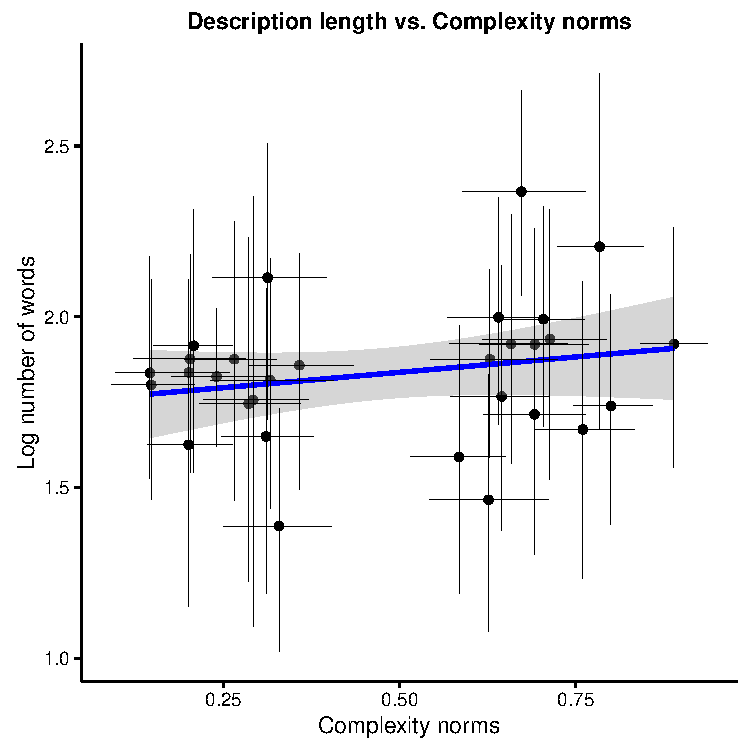
\includegraphics[width=4in]{figs/desc_length_word.pdf}
  \caption{\label{fig:desc_length} Relationship between description length and complexity norms. Error bars show  95\% confidence intervals.}
 \end{center}
\end{figure}


The key question was whether the description length was related to the psychological correlates of complexity measured in Chapter 2, explicit ratings and study times.
To test this question we fit a  linear mixed-effect model predicting log number of words with complexity norms as a fixed effect, and a second model predicting log number of words with study times as a fixed effect. As evident from Table~\ref{tab:sample_obj_descriptions}, participants varied considerably in the  syntactic construction of their descriptions as well as overall  length, making it important to control for this variability using a  mixed-effect model. The random effect structure included by-participant intercepts and by-trial slopes. There was a reliable relationship between log number of words and  complexity norms ($\beta=.2$, $t =2.8$; Fig~\ref{fig:desc_length}), and between log number of words and log study time ($\beta=.59$, $t =3.07$). The same pattern held for log number of characters. 

In the context of the Classical View of concepts, this result suggests a connection between conceptual complexity and number of primitives: More conceptually complex objects have longer descriptions, and thus more primitives. 

\section{Experiment 2a: Definitions of words}
Experiment 1 suggested objects that appear visually more complex are described with longer descriptions. The studies in Chapter 2, however, suggest that the construct of conceptual complexity extends beyond visual complexity to abstract word meanings. This predicts that the length of a dictionary definition of a word should be correlated with the conceptual complexity of its meaning. In light of the complexity bias observed in Chapter 2, we also predict that words with more complex definitions should be longer and have definitions that are rated as more complex. In Experiment 2 we tested these predictions by presenting participants with the definition of low frequency English words  and asking them to rate the conceptual complexity of the definition.

We selected low frequency words for several reasons. First, because participants were unlikely to know the word associated with the definition, knowledge of a word's length was unlikely to affect the complexity judgement. Second, because the words were uniformly low frequency, this reduced the possibility that differences in word length were due to frequency, rather than conceptual complexity. Finally, because participants were unlikely to know the words, we could conduct a follow-up experiment (2b) probing judgements about the length of a meaning's word, without knowledge of the English word interfering with this judgement.

\subsection{Methods}

\subsubsection{Participants} 
200 participants completed the task.

\subsubsection{Stimuli} 
We selected 100 dictionary definitions of low-frequency words (see Table~\ref{tab:sample_word_defs} for examples). 

\begin{table}[t!]
\centering

\begin{tabular}{ll}
\toprule
\textbf{Word} & \textbf{Definition}                \\
\toprule
   bissextile & ``a leap year"\\
   mussitation  &  \multicolumn{1}{p{12cm}}{ ``movement of the lips as if in speech but without accompanying sound"}    \\
   omphaloskepsis  &  \multicolumn{1}{p{12cm}}{ ``contemplation of one's navel as an aid to meditation"}                  \\
   parvis    &  \multicolumn{1}{p{12cm}}{ ``a court or enclosed space before a building"}                               \\
   sniddle      &  \multicolumn{1}{p{12cm}}{ ``long coarse grass"}     \\
   zarf     & \multicolumn{1}{p{12cm}}{ ``a holder, usually of ornamental metal, for a coffeecup without a handle"}                                 \\

 \bottomrule
\end{tabular}
\caption{Sample definitions of real English words used in Experiment 2.}
\label{tab:sample_word_defs}
\end{table}


\subsubsection{Procedure}
The task was identical to Experiment 9 in Chapter 2 (pg.\ \pageref{ch2-9}), except that participants were presented with definitions rather than words. Participants were first presented with instructions describing the norming task:
\begin{quote}
In this experiment, you will be shown the definition of a word and asked to decide how complex the meaning is. A word's meaning is simple if it is easy to understand and has few parts. An example of a simple meaning is ``brick.'' A word's meaning is complex if it is difficult to understand and has many parts. An example of a more complex meaning is ``engine.''
\end{quote}
For each definition, we then asked ``How complex is this definition?,'' and participants indicated their response on a 7-pt Likert scale anchored at ``simple'' and ``complex.'' The first two words were always ``ball'' and ``motherboard'' to anchor participants on the scale. Each participant rated a sample of 10 definitions. 

\subsection{Results and Discussion}
The central prediction is that definitions with more primitives in the definition, operationalized as the length of the definition, should be rated as conceptually more complex. To test this prediction, we fit a linear mixed-effect model predicting complexity ratings with log number of words in the definition as a fixed effect. The random effect structure included by-participant intercepts and by-trial slopes. As predicted, there was a strong relationship between complexity ratings and log number of words ($\beta=1.50$, $t =27.94$). The same pattern held for log number of characters.

A secondary prediction is that there should be a relationship between the length of the definition and the length of the word: If languages encode the conceptual complexity of a word's meaning in the length of the word, longer words should be associated with longer definitions. This prediction was not supported ($r=.05$, $p =.59$). Finally, we should also expect that  longer words should be associated with definitions rated as more complex. We fit the same mixed-effect model as above to test this prediction, except with log number of characters in the word as a fixed effect. There was a significant relationship between word length and rating judgements ($\beta=.52$, $t =2.86$), suggesting more complex definitions area associated with longer words. However, in a model with both word length and definition length as fixed effects, word length was no longer a reliable predictor of complexity ratings ($\beta=.18$, $t =1.19$).

In sum, we find a strong relationship between definition length and conceptual ratings, as predicted by Classical View of concepts: Longer definitions, with more primitives, are rated as more complex. We do not, however, find the predicted relationship between the conceptual complexity of the definition and word length, as would be predicted by the studies in Chapter 1.  One possible explanation for this null finding is that participants' complexity ratings were driven by the linguistic complexity of the definition, rather than its conceptual complexity. In other words, participants may have  rated longer definitions as more complex {\it because} they were longer, not because they were more conceptually complex. The current design does not allow us to distinguish these two possibilities.

\section{Experiment 2b: Definition mapping}
If definition length is related to conceptual complexity and participants have a complexity bias, we predict that participants should be biased to map more complex definitions on to longer words. In Experiment 2b, we test this prediction in an experiment analogous to the word mapping experiments in Chapter 2. Participants were presented with a meaning---a definition---and asked to guess the translation of the meaning in an alien language from two possible alternatives, one long and one short. 

\subsection{Methods}
\subsubsection{Participants} 
200 participants completed the experiment.
\subsubsection{Stimuli} 
We used the normed definitions from Experiment 2a. The short novel words contained one syllable, and the long novel words contained three syllables. There were 10 short and 10 long novel words presented in random order. 

\subsubsection{Procedure}
Participants were first presented with the following instructions:
\begin{quote}
In this experiment, you will see the definition of a word. Your job is to guess what the translation of that word is in an alien language. You will make your guess by betting on two possible words in the alien language. Imagine you have a \$100 dollars. To place your bet, assign an amount to each of the words. Your bets must add to 100.
\end{quote}
Participants then viewed a definition and two possible alternative words, one short and one long. Participants selected a response by placing a numeric bet (0-100) under each word.  Each participant rated 10 definitions in total. 

\subsection{Results and Discussion}
Consistent with previous evidence, we found a complexity bias in participants mappings from definition to words: Participants tended to map definitions rated as more complex in Experiment 2a to longer words ($r = .39$,  $p< .0001$). However, there was also a strong correlation between participants bets to longer words and definition length, measured in terms of log number of characters ($r = .82$, $p< .0001$). In an additive linear model predicting bets to the long word with both complexity norms and definition length, definition length ($\beta=3.81$, $t =2.64$, $p<.01$) was a significant predictor of bets, but complexity norms were not ($\beta=1.02$, $t =1.38$, $p=.17$). 

While this result is consistent with a complexity bias, as well as the pattern of complexity predicted by the Classical View of concepts, it is difficult to make strong causal inferences from these data. The fact that definition length accounts for more variance in bets than complexity norms suggests that it may be linguistic complexity, rather than conceptual complexity that is driving this bias. This result may simply reflect participants bias to map long definitions to long words. While a positive finding, this result does not speak to the claim directly that it is {\it conceptual} complexity per se that is related to definition length and the bias in word length. In Study 3, we try to address this issue more directly. 

\section{Study 3: Feature norms}
Study 3 provides tests the Classical View of complexity by examining the conceptual primitives of a concept through feature norms. Feature norms are collected by presenting participants with the name of a concept (e.g., ``moose") and asking them to produce as many features of the concept as possible (e.g., ``has for legs", ``has antlers"). If we assume that the features participants generate correspond to conceptual primitives in the definition of that concept, then the Classical View of concepts predicts that concepts with more  features should be more conceptually complex. If true, we should also expect concepts associated with more features to have longer labels. We test this prediction using a set of previously-collected feature norms.

\subsection{Method}
We analyzed feature norms for a set of 541 nouns \cite{mcrae2005semantic}. For each noun concept, we examined the relationship between the length of the word and the number of unique features participants listed for that concept. A feature was excluded from this measure if it was listed by fewer than 5 of 30 participants or described a taxonomic associate of the concept (subordinate or superordinate). Taxonomic associates were excluded because they are conceptually different than features which describe parts and functions. Word length was measured in terms of log number of characters. We also included spoken frequency of the target noun as a covariate in our models, measured from the Subtlex-us database \cite{brysbaert2009moving}. 

\subsection{Results and Discussion}
We first analyzed the simple correlation between word length and the number of features and found no relationship ($r=-.03$, $p=.54$)  However, spoken frequency is a strong, independent correlate of word length \cite{zipf1936}, and so it is important to control for this variability in measuring the relationship between number of features and word length. We fit an additive linear model predicting word length with both log spoken frequency and number of features.  There was a  relationship between number of features and word length (Fig.\ \ref{fig:feature_plot}): Longer words tended to have more features. Model parameters are presented in Table~\ref{study3amodel}.\footnote{We also fit the same model with the measure of number of features that included taxonomic features. In this model, the relationship between length and number of features was marginal ($\beta=0.08$, $t =1.92$, $p=.06$).} 

  \begin{figure}
 \begin{center}
  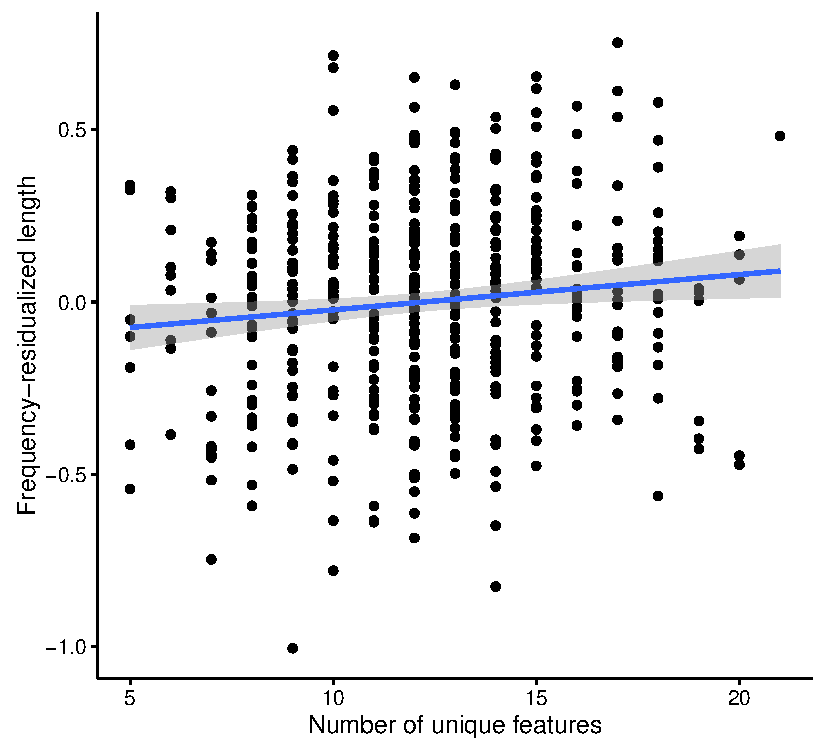
\includegraphics[width=4in]{figs/feature_plot.pdf}
  \caption{\label{fig:feature_plot} Study 3 results: Frequency-residualized word length (measured in log number of characters) as a function of the number of unique features associated with the concept a word denotes. }
 \end{center}
\end{figure}

% latex table generated in R 3.3.0 by xtable 1.8-2 package
% Mon Oct 10 13:57:56 2016
\begin{table}[t!]
\centering
\begin{tabular}{rrrrr}
  \hline
 & Estimate & SE & t-value & p-value \\ 
  \hline
(Intercept) & 2.2411 & 0.0638 & 35.13 & $<.001$ \\ 
  Num. features & 0.0112 & 0.0043 & 2.59 & $<.01$\\ 
  Log frequency & -0.2626 & 0.0214 & -12.29 & $<.001$  \\ 
   \hline
\end{tabular}
\caption{Model parameters for linear regression predicting word length in terms of number of features, controlling for word frequency.}
\label{study3amodel}
\end{table}

This finding is consistent with the Classical View, and suggests that conceptual complexity may be associated with the number of ``primitive" features associated with a concept.

\section{Study 4: Concept associates}
One limitation of Study 3 is the relatively small set of words used in the dataset. In Study 4, we aimed to replicate Study 3 with a larger dataset. We analyzed data from a word-association dataset in which participants were presented with a word asked to generate three ``related" words. This task differs notably from the feature norms in that participants were allowed to generate any word related to the target, not simply ``features" that describe conceptual parts. While this is a potential limitation of the current approach, we note that the distinction between features and associates is fuzzy. We find  the same pattern as in Study 3: Longer words tend to have more associates. 

The larger set of cue words in this dataset allowed us to also examine the relationship between the explicit complexity norms collected in  Experiment 9 in Chapter 2 (pg.\ \pageref{ch2-9}) and the number of associates. We reasoned that if the number of associates was related to conceptual complexity, as predicted by the Classical View,  these two variables should be positively correlated. This prediction was also supported.

\subsection{Method}
We analyzed an existing dataset containing word associations for  10,050 English words, collected from 73,256 participants \cite{de2013better}. The words include all grammatical classes. In the task, participants were presented with a cue and  asked to type ``the first  three words that came to mind." Each participant completed 15-19 trials. As in Study 3, we used a measure of spoken word frequency from the Subtlex-us database \cite{brysbaert2009moving}. 

\subsection{Results and Discussion}
We first tested for a relationship between log word length and number of unique associates: Word length was positively correlated with number of associates ($r = .11$, $p< .5$; see Table~\ref{study4corr} for all correlations).  Next, in order to control for the effect of word frequency on length, we fit an additive linear model predicting word length with number of associates and word frequency. Controlling for frequency, the relationship between number of associates and word length remained reliable ($\beta=0.004$, $t =27.34$, $p<.0001$; Fig.\ \ref{fig:associate_plot}).

Finally, we examined the relationship between the conceptual complexity norms from  Experiment 9 in Chapter 2  and number of associates. There were 431 words that overlapped between the two datasets. As predicted, there was a strong correlation between the conceptual complexity norms and number of associates: Words rated as more conceptually complex tended to have more associates ($r = .23$, $p< .0001$).


% latex table generated in R 3.3.0 by xtable 1.8-2 package
% Mon Oct 10 16:07:48 2016
\begin{table}[t!]
\centering
\begin{tabular}{llll}
  \hline
 & Log length (char.)  & Complexity norms &   Num. associates  \\ 
  \hline
Log length (char.) &  &  &  \\ 
Complexity norms  &  0.61**** &  &  \\ 
Num. associates &  0.11*    &  0.23**** &  \\ 
Log frequency& -0.54**** & -0.33**** &  0.18**** \\ 
   \hline
\end{tabular}
\caption{Pairwise correlations in Study 4. $p<.05$ = *; $p<.0001$ = ****}
\label{study4corr}
\end{table}

  \begin{figure}
 \begin{center}
  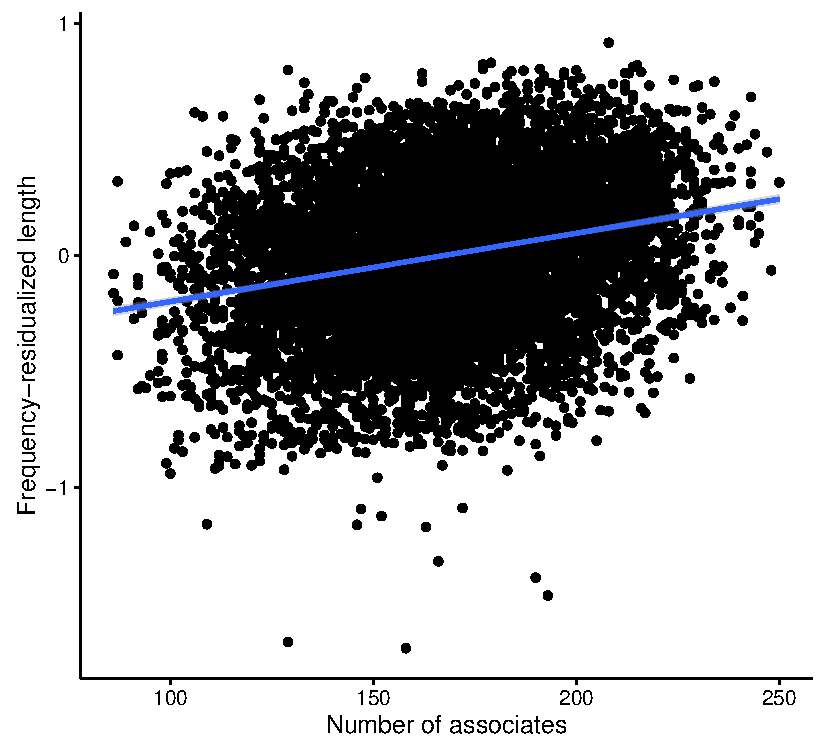
\includegraphics[width=4in]{figs/associate_plot.pdf}
  \caption{\label{fig:associate_plot} Study 4 results: Frequency-residualized word length (measured in log number of characters) as a function of the number of unique associates for a cue word. Each point corresponds to a word. For visualization, outliers three or more deviations above or below the mean were removed.}
 \end{center}
\end{figure} 

%Limit of this test of the classical approach -- assumes features are linguistically based; may not be true.

\section{Statistical View}
INTRO THE THEORIES
Exemplar + frequency
prototype + frequency
exemplar + variability
protype + variabiliyy

Exemplar Theory provides a second paradigm for considering the relative complexity of concepts. In this framework, a concept is represented as the set of individual exemplars observed of that category, with no additional compression of the concept in long term memory \cite<e.g.,>{medin1978context}. To operationalize complexity in this framework, we can again apply the description length criteria of Information Theory. If the primitives of representation are individual exemplars, then a more complex concept is one with more stored exemplars. W

How does frequency relate to concept learning. 
Evaluate: ease of learning model vs. transfer
Salthouse (1977): more exemplars increases recognition reaction time for letters, but NOT dot patterns (a concept) [same holds for accuracy)
Difference goes away with only a little bit of exposure
Argue there is an effect of number of exemplars only early in learning 

- More exemplars more transfer; worse memory for individual exemplars (see Omohunder, 1981; King and Newman, 1982)
- Familiarity speeds visual search paradigms (Wang, Cavaneough, Green 1994 ) 
- named famileiar matters more (Lupyan, 2008)


Salthouse (1977): more exemplars increases recognition reaction time for letters, but NOT dot patterns (a concept) [same holds for accuracy)
Difference goes away with only a little bit of exposure
Argue there is an effect of number of exmplars only early in learning 

\section{Experiment 5a: Simultaneous frequency}
We now turn to predictions about conceptual complexity from other theories of concepts: Exemplar and prototype theories. Both of these theories predict that aspects of experience should influence the representation of a concept, and thus the conceptual complexity of the concept. In particular, each makes predictions about the influence of observing individual exemplars of a concept.  Importantly, however, these two theories make different predictions about the direction of this influence. Under the exemplar theory, a participant who observes more exemplars of a concept consequently would have a representation of the concept that contained more individual exemplars. This is the case of an expert: A person who is a bird expert, for example, would have many exemplars of birds as part of the concept bird. This might mean that this concept has overall higher fidelity, than for a non-bird expert. Thus, the exemplar theory predicts that concepts with more observed exemplars will be more complex.

In contrast, the prototype theory predicts that participants represent only summary statistics over exemplars. If true, this means that the more exemplars a participant observes the less uncertainty there will be about the underlying concept; the concept prototype. Thus, the prototype theory predicts that the more exemplars a participant observes from a given concept, the {\it less} conceptually complex that concept will be. This prediction also falls out of an information theoretic account: Objects that appear more frequently are less surprising, and thus less conceptually complex.

In Experiment 5, we explore the possibility that the number of exemplars a participant observes influences the conceptual complexity of the concept. We present participants with either a few or many exemplars of a concept, and then ask participants to map that concept to either a short or long label. Under either theory, if conceptual complexity is related to exemplar frequency, we should expect the number of exemplars observed to influence how a concept is mapped to words of varying length. Under the exemplar theory, we expect long words to map to concepts with many exemplars, and under the prototype theory, we expect long words to map to concepts with few exemplars.

\subsection{Methods}
\subsubsection{Participants} 
477 participants completed the experiment.
\subsubsection{Stimuli} 
The objects were composed of a single geon, similar to those used in Expts.\ 1-3 in Chapter 2. The linguistic stimuli were novel words composed of either 2 (e.g., ``tupa," ``gabu," ``fepo")  or 4  (e.g., ``tupabugorn," ``gaburatum," ``fepolopus")  syllables.

\subsubsection{Procedure}
We presented participants with 10 objects on a single screen with a cover story that the objects were from a character's box (see Fig.\ \ref{fig:seqfreq_display} for precise text). Participants were required to click on a question mark to reveal each object. There were always two types of objects, one appearing nine times and the other once. Order of presentation was randomized.

After this training phase, participants completed a forced choice mapping task, as in Studies 1 and 5 in Chapter 2 (pg.\ \pageref{ch2-1} and pg.\ \pageref{ch2-5}). We presented a short or long word and asked participants to make a judgment about whether the word referred to the low or high frequency object. Each participant completed a single mapping trial, and word length was manipulated between participants.

 \begin{figure}
 \begin{center}
  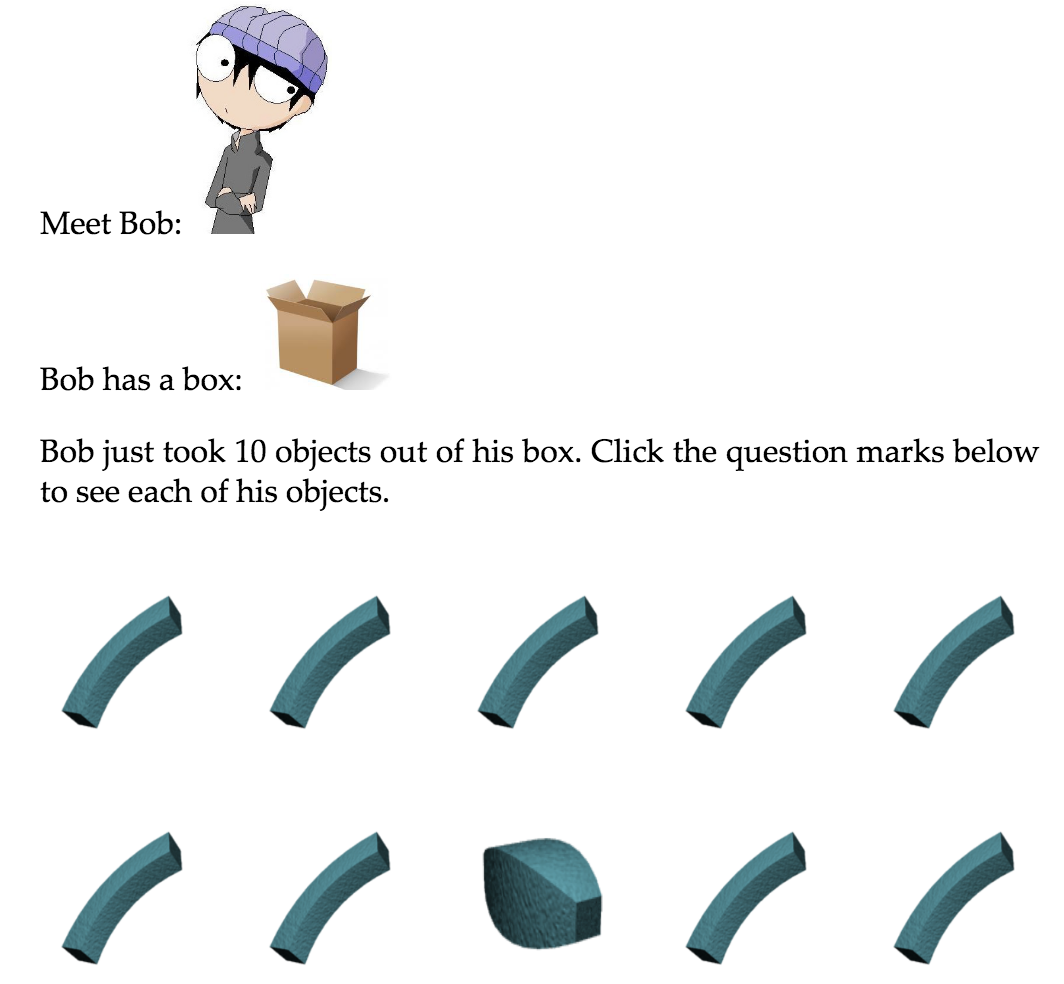
\includegraphics[width=3.5in]{figs/seqfreq_display.png}
  \caption{\label{fig:seqfreq_display} Sample display of the training phase in Experiment 5a.}
 \end{center}
\end{figure}


 \subsection{Results}
 Selections between the two conditions did not differ (${\chi}^2$$(1) = 0.02$, $p = .89$; Fig.\ \ref{fig:freq_plots}, left).
 
  \begin{figure}
 \begin{center}
  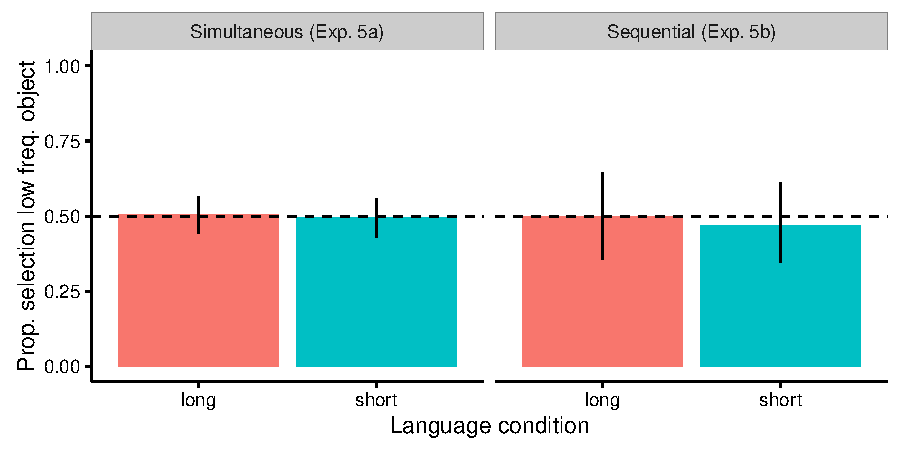
\includegraphics[width=6in]{figs/freq_plots.pdf}
  \caption{\label{fig:freq_plots} Proportion participants selecting the low frequency object as a function of language condition, in Exp.\ 5a (left) and Exp.\ 5b (right). Error bars are bootstrapped 95\% confidence intervals.}
 \end{center}
\end{figure}



\section{Experiment 5b: Sequential frequency}
Given the null finding in Experiment 5a, we next explore whether the timing of the presentation of exemplars affects complexity. Previous work has shown that participants may induce different concepts depending on whether or not exemplars are presented simultaneously, as in Exp.\ 5a,  or sequentially \cite<e.g.>{spencer2011}. In Experiment 5b, we present exemplars sequentially such that only one exemplar is visible at any given time. 

\subsection{Methods}
\subsubsection{Participants} 
97 participants completed the experiment.
\subsubsection{Stimuli} 

The objects were the set of novel, real objects used from Chapter 2, Expts.\ 4-6. 

\subsubsection{Procedure}
We manipulated object frequency by sequentially presenting objects. Participants saw 60 objects one at a time for 750 ms per object. One object was presented 10 times and a second object was presented 40 times. Ten additional objects were included as fillers, each appearing once. These were included to make the critical manipulation less obvious. Order of presentation was randomized. After this training phase, participants completed a single mapping trial as in Experiment 5a. Word length was manipulated between participants.

\subsection{Results and Discussion}
Selections between the two conditions did not differ (${\chi}^2$$(1) = 0.01$, $p = .92$; Fig.\ \ref{fig:freq_plots}, right). Across Expts.\ 5a and 5b, we find no evidence that the frequency of exemplars is related to the conceptual complexity of objects.

\section{Experiment 6: Facts}
In Experiment 6, we again test the hypothesis that the number of observed exemplars is related to conceptual complexity, as predicted by both the exemplar and prototype theories. However, in the present experiment, we explore the possibility that perhaps raw number of times an exemplar is observed is not the psychologically relevant dimension of frequency. We instead ask whether {\it conceptual} frequency, or markedness, is related to conceptual complexity by teaching participants facts about novel objects. We selected four categories of facts  that indicated the frequency of the object in the world, in a psychologically relevant way: Monetary cost, frequency of use, frequency of discussion, and frequency of appearance on Facebook (see Table \ref{tab:facts}).

\subsection{Methods}

\begin{table}[t!]
\centering

\begin{tabular}{ll}
\toprule
\textbf{Category} & \textbf{Fact}               \\
\toprule
   facebook & ``$\rule{1cm}{0.15mm}$s appear in the background of \{many/a couple\} pictures on Facebook."\\
   money  &  ``$\rule{1cm}{0.15mm}$s cost \{\$4/ \$400\}."   \\
   talk  & ``$\rule{1cm}{0.15mm}$s get talked about once a \{day/year\}." \\
   use    & ``$\rule{1cm}{0.15mm}$s are used once a \{day/year\}."                             \\

 \bottomrule
\end{tabular}
\caption{The eight facts used in Experiment 6. For each of the four categories, there was a high and low frequency alternate (shown in  brackets).}
\label{tab:facts}
\end{table}

\subsubsection{Participants} 
120 participants completed this experiment. 

\subsubsection{Stimuli} 
All participants were presented with the same eight facts, shown in Table \ref{tab:facts}. Objects were again a sample of the novel, real objects used in Chapter 2, Expts.\ 4-6.  The novel words were identical to Exp. 5.

\subsubsection{Procedure}
Participants were presented with the following instructions:

\begin{quote}
In this experiment, you will learn facts about objects but the name of the object will be missing. For example, a fact like, ``Mops are used for cleaning the floor," will appear as ``$\rule{1cm}{0.15mm}$s are used for cleaning the floor." After you memorize these facts, you will then be asked to guess the name for each object. 
\end{quote}
Participants  then saw  all 8 facts paired with an object. The facts appeared just as in  Table \ref{tab:facts}, with a blank for the name of the object. Participants were allowed to study the fact-object pairings for as long as they wanted. They then proceeded to a test phase where  each object was shown next to a multiple choice set of all 8 facts. For each object, participants had to select which fact from the training phase was true of that object. Participants were then given feedback about their responses, and repeated the study and test phase until all 8 facts were correctly recalled. 

Next, participants completed a mapping task as in previous experiments. Participants saw a novel word and two objects and were asked to guess which object the word referred to. Each participant completed four mapping trials, two with long words and two with short words. The pairs of objects in each trial were from the same fact category (``facebook," ``money," ``talk," or ``use"). Thus, each trial required participants to make a judgement about the meaning of a word between a low  and high conceptutally-frequent object. Order of categories was counterbalanced across participants. Word lengths were randomized across trials. 

\subsection{Results and Discussion}
Participants studied and completed the test a mean 2.4 times ($SD = 1.49$).  Across all four categories, there was no evidence that selections to the short or long word varied as a function of the frequency valence of the fact (all ${\chi}^2$$(1) < 3.8$; $p > .5$). Results did not differ as a function of how many times participants studied the facts. In sum, then, across both Experiments 5 and 6, we find no evidence that exemplar frequency, either objective  or psychological, is related to conceptual complexity. Next we turn to a final hypothesis about the nature of conceptual complexity: exemplar variability.

  \begin{figure}
 \begin{center}
  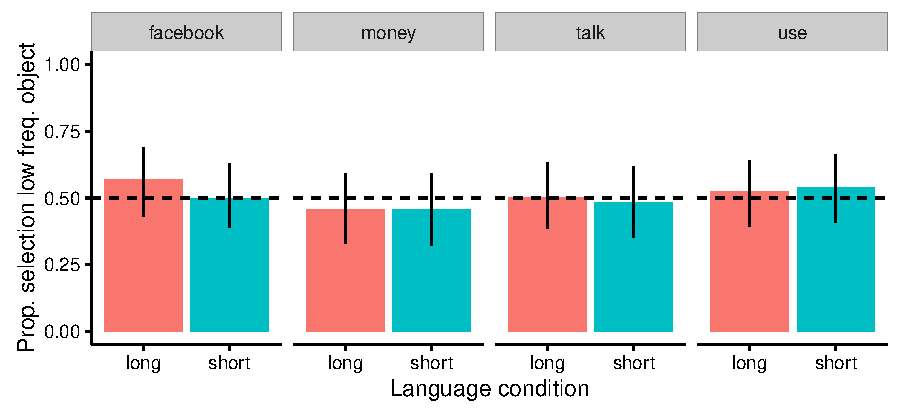
\includegraphics[width=6in]{figs/fact_plots.pdf}
  \caption{\label{fig:fact_plots} Experiment 6 results: Proportion participants selecting the object associated with the low frequency fact as a function of fact category and language condition. See Table \ref{tab:facts} for explanation of fact categories. Error bars are bootstrapped 95\% confidence intervals.}
 \end{center}
\end{figure}

\section{Experiment 7: Exemplar variability}
The final hypothesis about conceptual complexity derives from the Prototype Theory of concepts: A concept is conceptually complex if its exemplars are highly variable. This is predicted by 

cite haskell

\subsection{Methods}
\subsubsection{Participants}

396 participants completed the experiment.

\subsubsection{Stimuli} 
The linguistic stimuli were identical to previous experiments. There were four classes of object stimuli (bugs, birds, flowers, and fish). Each participant saw 10 objects from two classes. For each object class, two features varied continuously (e.g. for bugs, body and head size). Size parameters for the low variability objects were  sampled from a low variability distribution, and size parameters for the high variability objects were  sampled from a high variability distribution (see Fig.\ \ref{fig:var_screen_shot} for sample stimuli sets).

\subsubsection{Procedure}
The procedure was identical to Exp. 5a, with the exception of the training display. During the training phase, participants were given the following instructions:

\begin{quote}
In the country of Desodonia, there are two different \{forests/forests/fields/lakes\}. Each \{forest/forest/field/lake\}  is home to a different kind of \{bug/bird/flower/fish\}. To see some of the \{bugs/birds/flowers/fish\} in each \{forest/forest/field/lake\}, click the question marks below.
\end{quote}

They then saw two 5-by-2 grids of question marks corresponding to two different forests, fields, or lakes. The object was revealed after the participant clicked on the question mark. After all question marks had been clicked, the final display appeared as in Fig.\ \ref{fig:var_screen_shot}. After this training phase, participants advanced to a single word mapping trial as in Exp. 5a. 


  \begin{figure}
 \begin{center}
  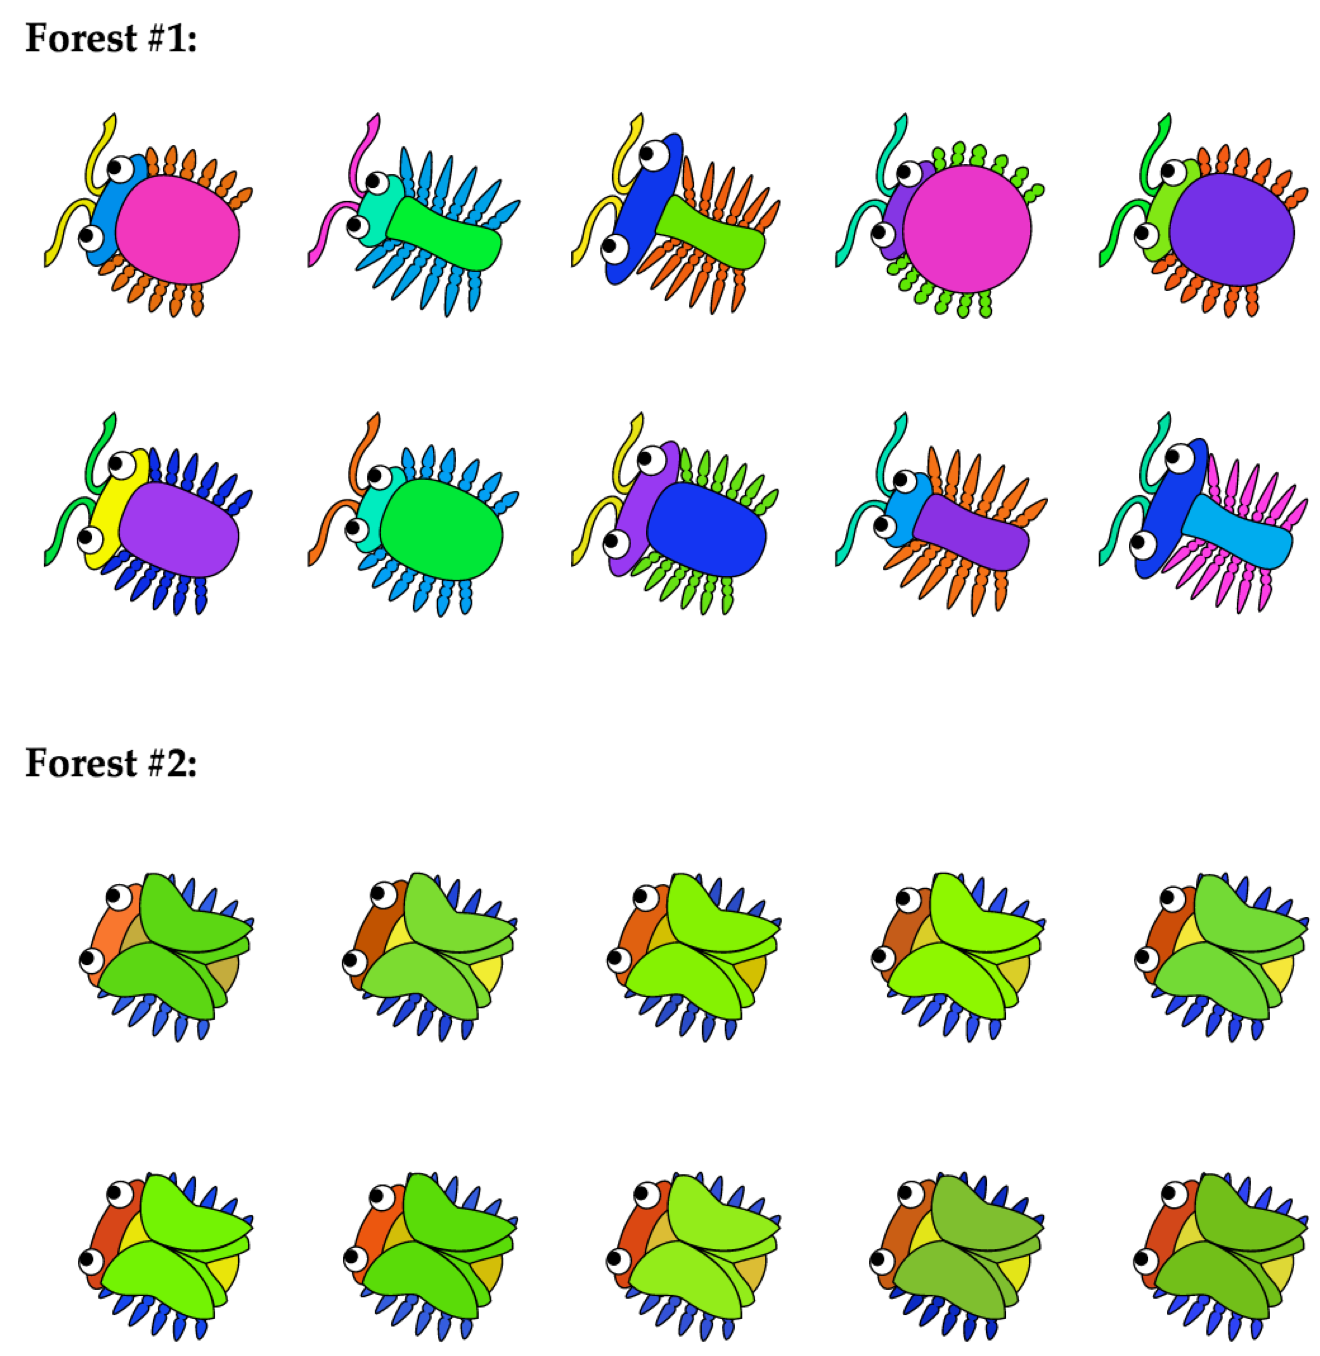
\includegraphics[width=4in]{figs/var_screen_shot.png}
  \caption{\label{fig:var_screen_shot} Example stimuli sets in Experiment 7. High variability bugs are shown on top (Forest \#1) and low variability on bottom (Forest \# 2).}
 \end{center}
\end{figure}



\subsection{Results and Discussion}

Selections of the high variability object did not differ as a function of word length (${\chi}^2$$(1) = 1.12$, $p = .29$; Fig.\ \ref{fig:var_plot}). However, 70 participants failed to correctly recall which category member was from the high-variability category, suggesting that participants may not have even noticed the critical manipulation. Nevertheless, even with these participants excluded, there was no difference between conditions (${\chi}^2$$(1) = .05$, $p = .82$).

  \begin{figure}
 \begin{center}
  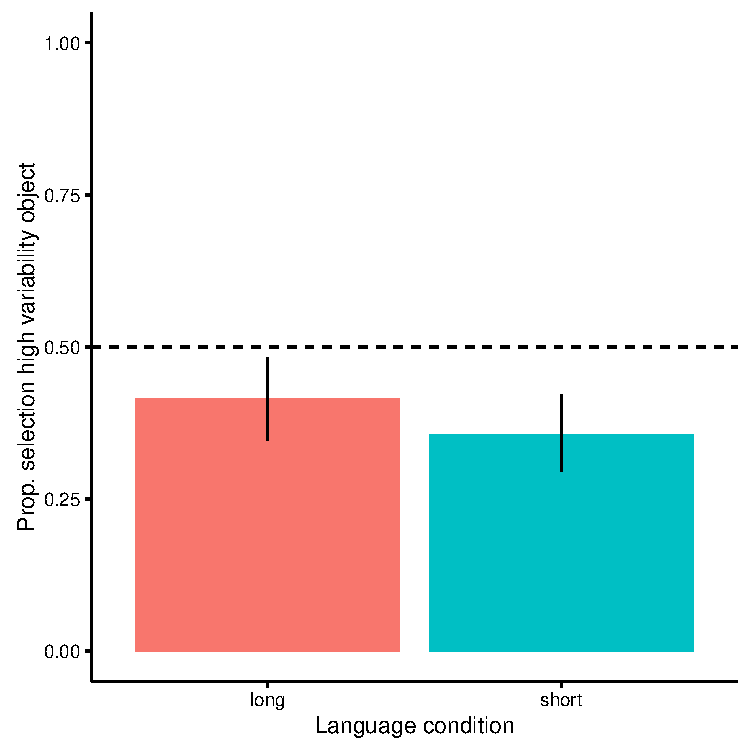
\includegraphics[width=4in]{figs/var_results.pdf}
  \caption{\label{fig:var_plot} Experiment 7 results: Proportion participants selecting the object associated with the high variability fact as a function language condition.  Error bars are bootstrapped 95\% confidence intervals.}
 \end{center}
\end{figure}

\subsection{Conclusion}










%!TEX root = ../dissertation.tex

\chapter{Origins of a complexity bias}
\label{chapter:origins}

\section{Introduction}

A universal property of languages is that they contain units of meaningful sounds---words---that vary in length. What accounts for this variability? That is, why is the word for ``can'' short but the word for ``calculator'' long? One class of explanations for this variability appeals to properties of the linguistic form itself, such as word frequency \cite{zipf1936} and predictability in linguistic context \cite{piantadosi2011a,mahowald2013info}. Our recent work has revealed an additional factor influencing word length: conceptual complexity. Across 80 natural languages, we find a bias for longer words to refer to conceptually more complex meanings ({\it complexity bias}; Chapter 2). This systematicity between word length and meaning challenges the long-held assumption that the relationship between form and meaning is entirely arbitrary \cite{saussure}.

In Chapter 4, we turn away from the question of what conceptual complexity is to the question of {\it why}: Why is there a complexity bias in the lexica of natural languages? We take as the central datum to be explained the bias in natural language for longer words to map onto more complex meanings (Studies 9 and 10 in Chapter 2).  To answer this question, we first consider the hypothesis space of the origins of a complexity bias in the lexicon. We then present a series of four studies that shed light on the relative likelihood of these different hypotheses.\footnote{Parts of this chapter are published in  Lewis, M. \& Frank, M. C. (2015). Conceptual complexity and the evolution of the lexicon. Proceedings of the 37th Annual Meeting of the Cognitive Science Society (p. 1138-1343). Austin, TX: Cognitive Science Society, and in,  Lewis, M., Sugarman, E., \& Frank, M. C. (2014). The structure of the lexicon reflects principles of communication. Proceedings of the 36th Annual Meeting of the Cognitive Science Society (p. 845-850). Austin, TX: Cognitive Science Society.}


\subsection{Hypotheses about the origins of a complexity bias}
The conceptual framework of  timescales is useful in understanding the space of hypotheses about the origins of a complexity bias. We assume that a complexity bias in natural language emerges at the timescale of language evolution. Critically, we also assume that the bias at the timescale of language evolution must have emerged---at some point---as the product of processes at shorter timescales, even if indirectly. In particular, we consider pressures at the timescales of language use and development. Below we describe four different hypotheses of pressures at shorter timescales that would, over time, lead to a complexity bias in the lexica of natural languages at the evolution timescale. These pressures are summarized in Table \ref{tab:bias_hypotheses}.


\hspace*{.3 cm}{ \it 1.\ The Efficient Naming Hypothesis.} To understand one variant of this hypothesis, consider the following fable: At the beginning of linguistic time, names were assigned to objects by length, starting with the shortest. Objects were named in the order that they were observed or as they became communicatively relevant. Since more frequent or communicatively-relevant objects  tended to be observed earlier, these objects received shorter names, relative to the less frequent objects that were encountered later.   The result is a language the contains a complexity bias in its lexicon.




\bgroup
\def\arraystretch{1.5}% 

\begin{table}[t!]
%\footnotesize
\centering
\begin{tabular}{l l l l l }
 \toprule
 \textbf{Hypothesis} &  \textbf{Pressure}& \textbf{\begin{tabular}[c]{@{}l@{}}Relevant\\Study\end{tabular}} \\
 \toprule
Efficient Naming Hypothesis   & \multicolumn{1}{p{8cm}}{Bias to name simple meanings  first {\it and} coin short words first.} & Study 1\\
Learning Hypothesis &  \multicolumn{1}{p{8cm}}{A lexicon with a complexity bias is more learnable.} & Study 2 \\
Memory Hypothesis & \multicolumn{1}{p{8cm}}{Speakers make memory errors by mis-remembering simpler meanings with shorter words.} & Study 3  \\
Pragmatic Hypothesis & \multicolumn{1}{p{8cm}}{ Speakers truncate simpler meanings with shorter words in order to facilitate communication.} & Study 4 \\

 \bottomrule
\end{tabular}
\caption{Summary of origin hypotheses and relevant studies.}
\label{tab:bias_hypotheses}
\end{table}
\egroup

%This story provides one possible account of the emergence of a complexity bias over the language evolution timescale.

This hypothesis posits two independent pressures operating at shorter timescales: The bias to name simple objects first and the bias to coin short words first. Both of these pressures could be due to pragmatic or cognitive demands. Importantly, however, the Efficient Naming Hypothesis suggests that the complexity bias in natural language is not directly reflected in psychological phenomena (the mind does not have a ``complexity bias"), but rather that the bias in natural language is epiphenomenal to psychological processes.

\hspace*{.3 cm}{ \it 2.\ The Learning Hypothesis.} 
A second possibility is that the pressure shaping the lexicon operates over the developmental timescale due to learning constraints: When learning the meaning of words, children are better able to learn a lexicon that tends to map complex meanings to long words and simple meanings to short words. Why might children have this bias? One possible account is that children have a bias to assume that there is resemblance between the form of a word and its meaning; that is, a bias for iconicity. There is a large literature suggesting that lexica of natural language indeed contain some degree of iconicity  \cite<see>[for review]{schmidtke2014phonological}. 

In addition, there is evidence suggesting that iconicity may facilitate word learning. For example, \citeA{imai2008sound} found that Japanese children were better able to acquire novel words that were iconically related their referents, relative to non-iconic words.\footnote{There is also some evidence to suggest that children may show the ``bouba-kiki`` effect \cite<the bias to map the word ``bouba" onto a curvy object, and ``kiki" onto a pointy object; e.g.,>{maurer2006shape}, but a recent meta-analysis of this literature suggests that this bias may not be robust in children \cite{lammertink2016}.} More broadly, in an analysis of early learned words, recent work suggests a relationship between the iconicity of a word and age of acquisition: In particular, more iconic words tend to be learned earlier \cite{perry2015iconicity}.

Thus, under this hypothesis, an iconic bias to map more complex meanings onto longer words exerts pressure over the timescale of development. Over language evolution, this learning pressure leads to a lexicon that facilitates learning by encoding a complexity bias. 

%This hypothesis is consonant with the broader proposal that language is shaped by learning pressures \cite{}

\hspace*{.3 cm}{ \it 3.\ The Memory Hypothesis.} This hypothesis posits that a cognitive bias, such as a bias for iconicity, exerts pressure on memory at the in-the-moment timescale. More specifically, a psychological bias for iconicity causes small changes in memory for complex phonological forms in the moment of language interaction, and  this  pressure leads to biases in linguistic transmission across generations. Over the course of language evolution, these psychological, synchronic biases result in a lexicon that magnifies this bias  \cite{griffiths2007language}. 

%Over time, this behavioral regularity might become a probabilistic rule,  becoming ``grammaticalized'' into the language. 

\hspace*{.3 cm}{ \it 4.\ The Pragmatic Hypothesis. } A final possibility is that humans are predisposed to consider the intentions of others \cite{tomasello2005understanding}. This predisposition leads to pragmatic reasoning. As argued by \citeA{horn1984}, one type of inference that might be guided by pragmatic reasoning is that a costlier (i.e.\ longer) utterance is more likely to refer to a more complex meaning, than a shorter one. Thus, under this hypothesis, domain-general pragmatic reasoning may underly an in-the-moment complexity bias. Over time, this in-the-moment bias may become grammaticalized, leading to a complexity bias in the lexicon. This possibility is consistent with other work showing that features of the lexicon also reflect principles of communication, like the structure of semantic space \cite{regier2007color,kemp2012kinship,piantadosi2012communicative}. 

%A second alternative is that the bias  is related to principles of communication.   As part of a broader theory of communication, \citeA{horn1984} suggested that a contrast in length between two phrases with the same denotational value implies a contrast in meaning, with the longer phrase getting the more unusual or complex meaning. Thus, the complexity bias  in the lexicon could reflect this in-the-moment communicative bias---

%A variant of this hypothesis is that an in-the-moment behavioral bias might be the product of both an underlying pragmatic inference and an overhypothesis about a complexity regularity in the lexicon. This possibility is similar to one account of a different, well-studied bias in word learning \cite{lewis2013b}: the mutual exclusivity bias. The mutual exclusivity bias is the tendency for children to map a novel word onto a novel object. In this work, we suggest that the mutual exclusivity behavior may emerge from both an in-the-moment pragmatic inference (the speaker would have used the known word to refer to a known object if that was the intended referent,  and so the novel word must refer to the novel object) and an overhypothesis about the structure of the lexicon (a 1-1 mapping between words and concepts).  We argued that processes at both timescales may jointly contribute to mutual exclusivity behavior. 

Importantly, these possibilities are not mutually exclusive with each other. In principle, all four of these hypotheses could simultaneously be correct and mutually enforcing. More likely, several of these might be true, perhaps with different weights. For example, speakers might have a bias for iconicity, which might lead to {\it both} memory errors and a learning bias. Furthermore, these different hypotheses may be causally related to each other: An iconic bias might lead to a pragmatic bias (i.e.\ if the speaker knows the listener is biased to assume that a long word refers to a complex meaning, then a helpful speaker will use that mapping). Indeed, there are a number of different hybrid accounts that can be derived from this space of possibilities. A final issue is how the in-the-moment bias---as evidenced by our novel word mapping experiments in Chapter 2---is accounted for. This issue is related to the account of the bias in natural language, though the accounts need not necessarily be the same. We return to this issue in the General Discussion.

In the present chapter, we appeal to data from four studies to shed light on the likelihood of these different hypotheses. In Study 1, we examine whether there is a complexity bias in a large sample of languages with primitive words. In Study 2, we ask whether this bias is present in language acquisition over the course of development. Finally, in Studies 3 and 4, we ask whether memory and pragmatic pressures might influence the emergence of a complexity bias in the lexicon. Taken together, we find that these data are most consistent with the Memory and Learning Hypotheses. 


%%%%%%%%STUDY 1-SWADESH%%%%%%%%
\section{Study 1a: Complexity norms for primitive words}
As a first step in exploring the origins of the complexity bias, we sought to replicate and extend our previous work suggesting that a lexical complexity bias was present in a diverse set of languages (Study 10, Chapter 2, pg.\ \pageref{ch2-10}). We also sought to test one prediction of the Efficient Naming Hypothesis. Recall that the Efficient Naming Hypothesis assumes that  meanings with high ``communicative need" should be named first, and that they should receive short labels. This thus predicts that words with high communicative need should not tend  to show a complexity bias cross-linguistically. Instead, they should all be named with relatively short words.

With these goals, we examined the complexity bias within a list of high communicative need words  developed by  \citeA{swadesh1955towards}, across a large sample of languages. We selected this list of words because it was developed explicitly to contain words that were conceptually primitive and therefore likely to have direct translation equivalents across languages. While similar, it is important for interpretation to note that the present study differs from Study 9 in Chapter 2 in several ways. First, the present study considers a much larger set of languages (80 vs.\ 1,037), but a smaller set of words (499 vs.\ 40). The words in the present sample are higher frequency and more conceptually primitive than the words in Study 9, and thus likely to have been borrowed from other languages. The words in the present sample also have less variability in word length. Finally, in the present study, we use a different metric of word length---phonetic code length rather than number of characters---to quantify length. This has the advantage of more closely resembling the spoken word, but nevertheless makes the two studies less comparable. This differences suggest we should be cautious in directly comparing the two samples. 

In Study 1a, we ask participants to rate the conceptual complexity of each of the word meanings on the Swadesh list, using a procedure similar to Study 9 in Chapter 2. Averaging across participants, we  estimate the conceptual complexity of each word in this sample.  In Study 1b, we then consider the translation equivalents of these words across 1,037 languages and ask how variability in conceptual complexity is related to word length in each language. If the Efficient Naming Hypothesis is correct, we should not expect to observe a robust complexity bias in this sample of words. Contra this prediction, we find a complexity bias in this large sample of languages, but smaller than in Study 10 with a different sample of words and languages.

%If the complexity bias in natural language observed in Study 9 in Chapter 2 is a robust phenomenon, we should expect the bias to extend to this new set of words and this broader sample of languages. 

\subsection{Method}
\subsubsection{Participants} We recruited 100 participants from Amazon Mechanical Turk.
\subsubsection{Stimuli}
We presented participants with subset of the word list developed by \citeA{swadesh1955towards}. This list was developed  for the purpose of inferring genetic relations between languages on the basis of their lexical similarity. The original list contains 100 meanings that are considered ``core vocabulary," and thus likely to be present in all languages (e.g., natural objects, colors, body parts). More recently, this list has been used in a project that aims to automatically generate language classifications on the basis of similarity between word lists \cite{brown2008automated}. In this project, it was found that comparable accuracy in classification could be achieved by using a subset of the original list, a 40-item list \cite{holman2008explorations}. The primary advantage of this smaller list is that translations are available for a much larger sample of languages. Thus, we adopted this 40-item word list in our work here (see Table~\ref{tab:swadeshwords} for full list of items). Each participant rated all 40 words from the  Swadesh word list. 

\begin{table}[t!]
\centering
\begin{tabular}{llllllll}
 \hline
blood  &  bone   &  breast   & come &    die    &  dog &     drink &  ear   \\
eye   &   fire   &  fish    & full   &  hand  &   hear &    horn  &   I  \\
knee  &   leaf   &  liver  &  louse  &  mountain  &name   &  new   &   night  \\
nose     &one    &  path     &person  & see    &  skin &    star  &   stone \\
sun  &    tongue  & tooth  & tree &    two      &water &   we    &   you     \\
 \hline
\end{tabular}
\caption{List of 40 Swadesh words.}
\label{tab:swadeshwords}
\end{table}

\subsubsection{Procedure}
We used the same norming procedure as in Study 9 in Chapter 2 (pg.\ \pageref{ch2-9}), with a few minor changes. In this version, participants were not given examples in the instructions and did not complete anchor trials.\footnote{A previous version of the experiment included instructions identical to Study 9 in Chapter 2. With these instructions, we find that there was limited variability in responses because all of the words were relatively conceptually simple, relative to the complex example and anchor item. Nevertheless, we also see a complexity bias in this sample, but smaller in magnitude ($r=0.32, p<.001$).} The full instructions seen by participants are presented below.  
\begin{quote}
In this experiment, you will be asked to decide how complex the meaning of a word is. A word's meaning is simple if it has few parts. A word's meaning is complex if it has many parts.
\end{quote}
For each word, we then asked ``How complex is the meaning of this word?,'' and participants indicated their response on a 7-pt Likert scale anchored at ``simple'' and ``complex.''

\subsection{Results and Discussion}
For each item, we calculated the mean complexity rating across participants ($M = .44$; $SD = 2.53$). We then used these ratings to estimate the complexity bias in the sample of words. We quantified word length in terms of number of characters. Consistent with previous studies, we find a positive correlation between word length and conceptual complexity ($r=0.51$, $p<.001$; Figure\ \ref{fig:study1a}). In Study 1b, we ask whether this relationship holds for a large sample of diverse languages.

\begin{figure*}[t!]
\begin{center}
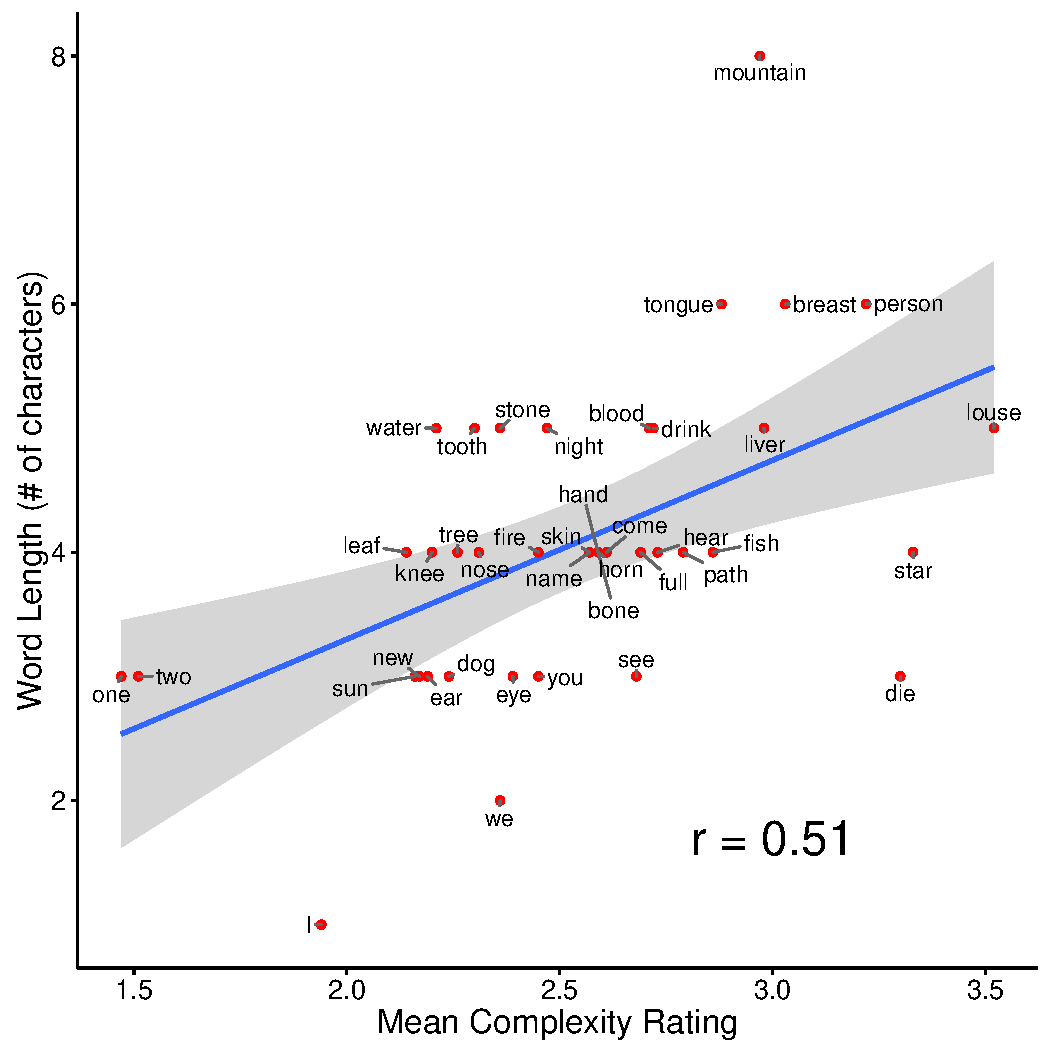
\includegraphics[scale = .6]{figs/chap4_1a.pdf}
\end{center}
\caption{Word length as a function of complexity norms for items in the 40-item Swadesh word list.}
\label{fig:study1a}
\end{figure*}


\section{Study 1b: Complexity bias for primitive words}

\begin{figure*}[t!]
\begin{center}
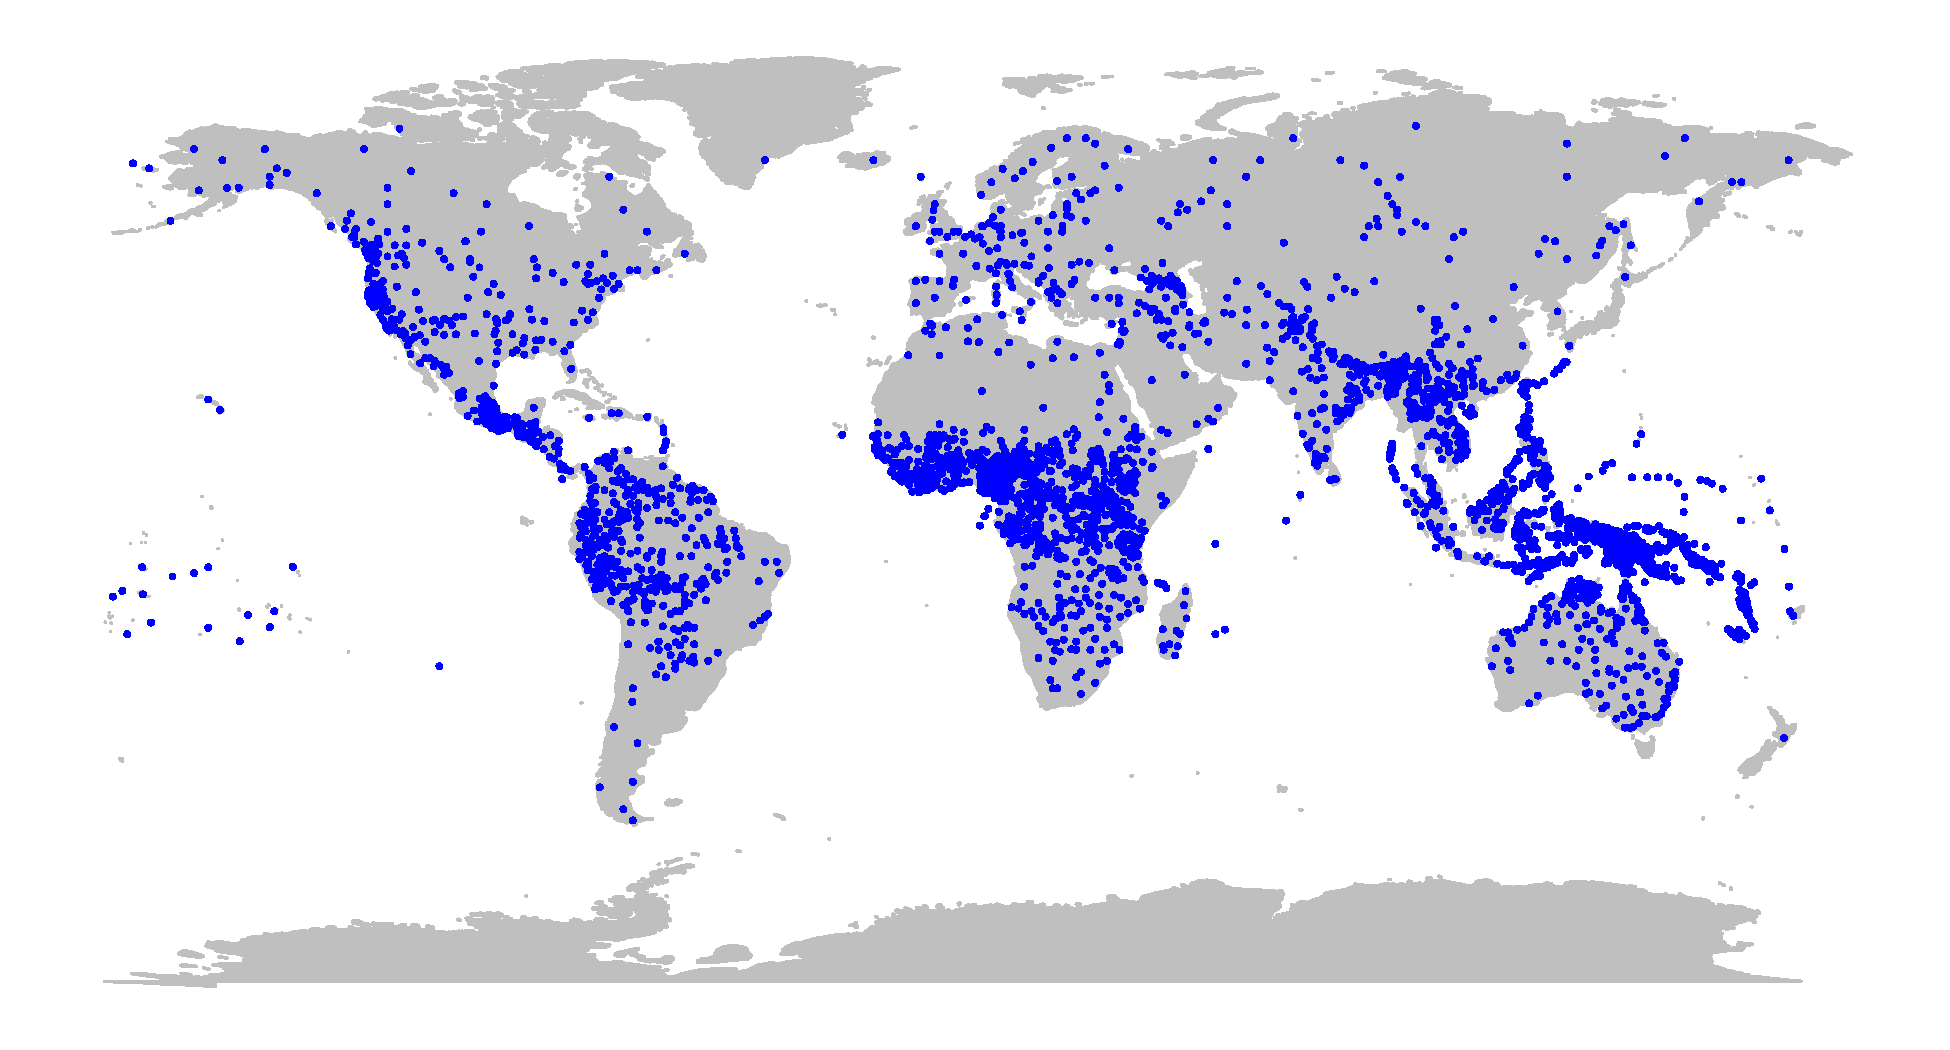
\includegraphics[scale = .45]{figs/chap4_1map.pdf}
\end{center}
\caption{Geographical distribution of languages in Study 1b. Each point corresponds to a language.}
\label{fig:study1b_map}
\end{figure*}

\subsection{Method}
To estimate the complexity bias cross-linguistically in this sample, we analyzed translations of the 40-item list in the  ASJP database \cite{asjp}. This database contains translations for the list of 40 words for 1037 languages from 261 distinct language families. The geographical distribution of the languages is shown in Figure\ \ref{fig:study1b_map}. For cross-linguistic comparability, this database transcribes words using a simplified version of International Phonetic Alphabet, called ASJPcode. In our analyses, we thus measure word length in terms of number of ASJP characters.

\subsection{Results}
For each language, we calculated the correlation between word lengths and complexity norms for the sample of 40 words. The distribution of correlations is shown in  
Figure\ \ref{fig:study1b} ($M = .12$; $SD = .17$). The magnitude of this correlation is affected slightly by the distribution of word lengths in each language, due to restriction of range. We corrected for this bias by calculating the maximum possible correlation between complexity ratings and word lengths in each language, and then normalizing the observed correlation by this maximum value. With this correction, the mean correlation was slightly larger ($M = .13$; $SD = .18$). 

\begin{figure*}[t!]
\begin{center}
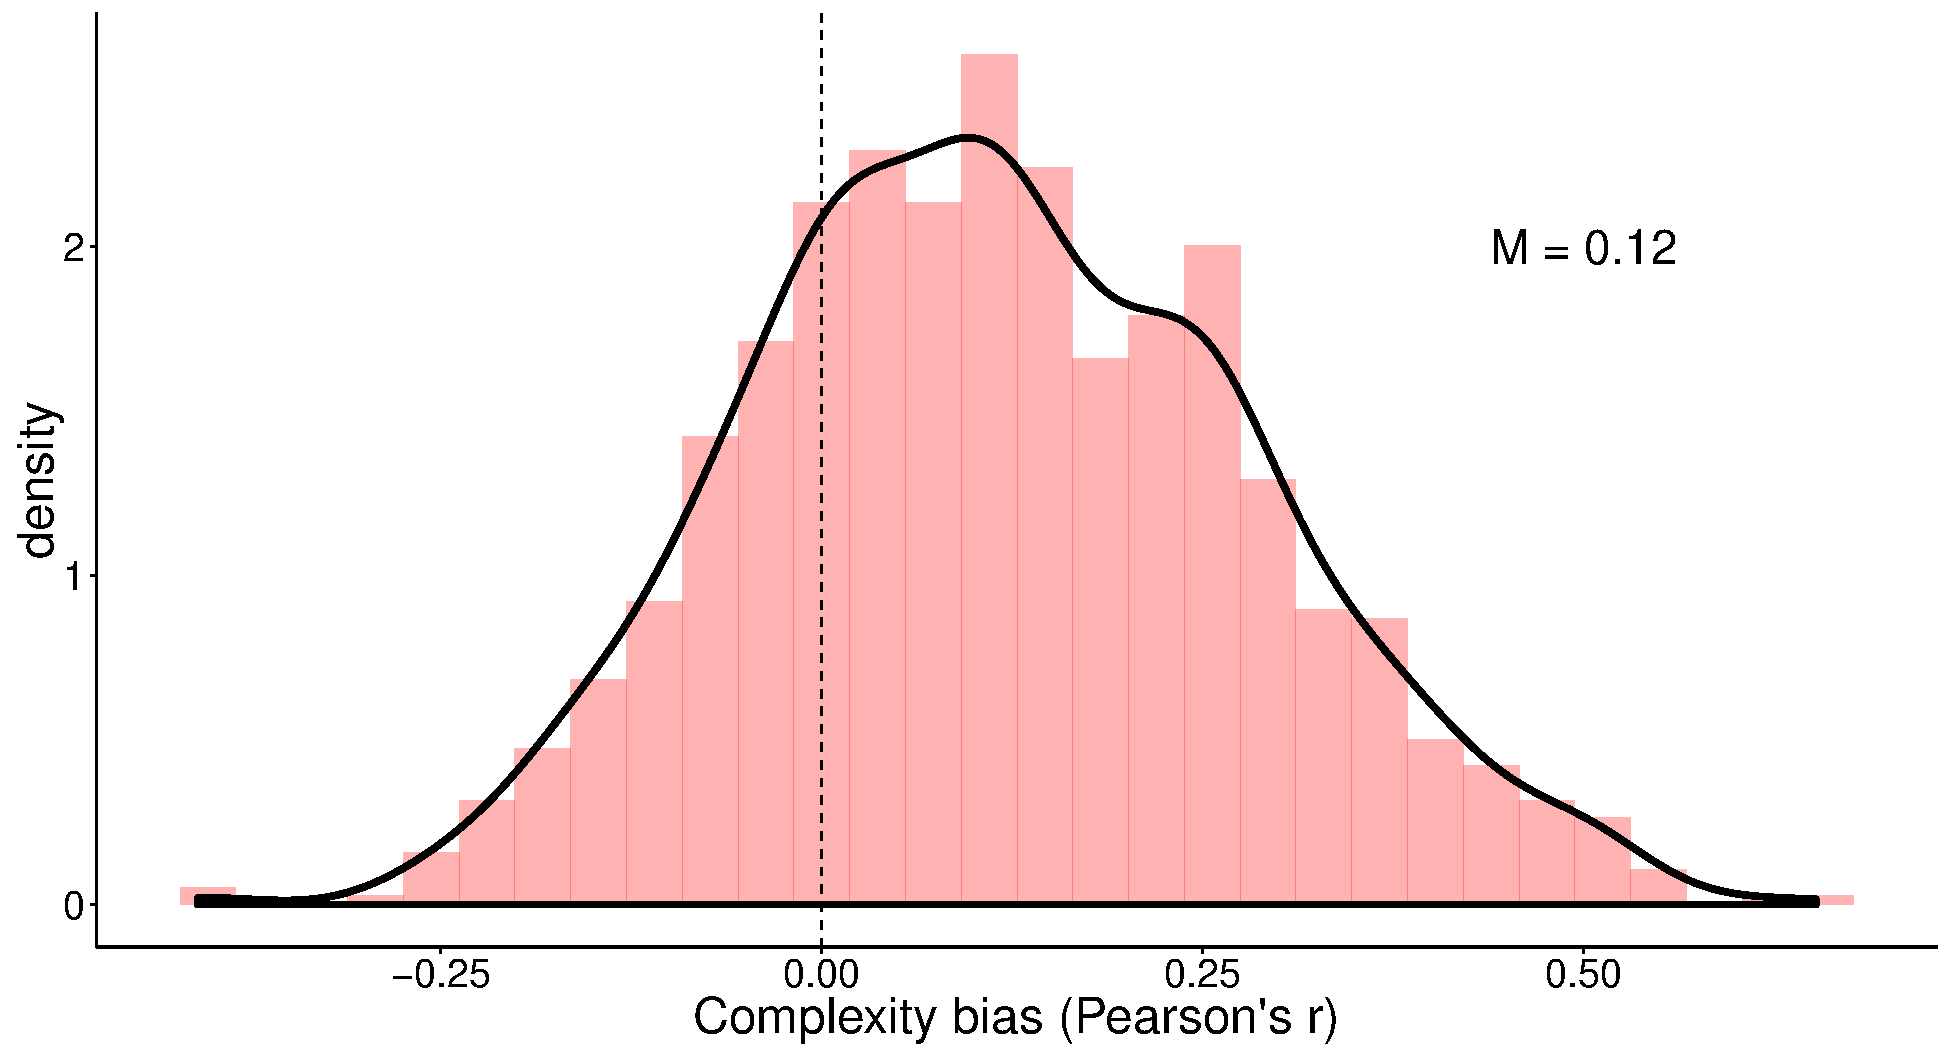
\includegraphics[scale = .35]{figs/chap4_1b.pdf}
\end{center}
\caption{For each language, we calculated the correlation coefficients between word length and complexity norms for the set of 40 words. This plot shows the distribution of correlation coefficients across all 1,037 languages. }
\label{fig:study1b}
\end{figure*}


Across languages,  the correlation significantly differed from zero ($ t(1036)= 22.87$; $p <.0001$).  To control for the non-independence of languages from the same linguistic family, we constructed a mixed-effect linear model predicting word length with complexity bias as a fixed effect. The random-effect structure included language and language family as both random slopes and intercepts.\footnote{The model specification was as follows: \texttt{word length $\sim$ complexity + (1 + complexity ~\textbar~language family) +  (1 + complexity ~\textbar~language)}. This was the maximal random effect structure that allowed the model to converge.}  The model showed a significant effect of complexity on length ($\beta = .18$, $t = 5.6$), suggesting that the complexity bias is present across a range of diverse languages.

We next compared these results to those observed in the sample of 499 words using Google Translate from Study 10 in Chapter 2 (pg.\ \pageref{ch2-10}). Across languages, the mean correlation between length and complexity norms was larger in the Study 10 sample ($M = .34$; $SD = .12$), compared to the current sample ($M = .12$; $SD = .17$). One potential source of this difference could be the degree of sampling error between the two samples: In the sample from Study 10, each language contained 499 words, whereas in the current sample, each language contains only 40 words. To control for this difference, we sampled 40 words from the words from Study 10 and recomputed  the mean correlation across languages. The down-sampled mean was comparable to the original  ($M = .34$; $SD = .17$). 

\subsection{Discussion}

In Study 1b, we replicate our finding from Study 10 in Chapter 2 with a larger and more diverse set of languages. In addition, the fact that we find this bias in a sample of high frequency, high communicative need words, provides some evidence against the Efficient Naming Hypothesis as the origin of the complexity bias in natural language.

As described above, the present study and Study 10 (Chapter 2) differ in many ways, making a direct comparison between the two samples difficult. Nevertheless, our best guess is that the overall mean correlation in the present sample is approximately .22  smaller than that in Study 10.  There are a couple possible explanations of this difference. The first is that a complexity bias is smaller in high frequency words, perhaps because high frequency words are most affected by other pressures in the linguistic system \cite{lieberman2007quantifying}. A second possibility is that because our norms were collected in English, we are better able to capture the conceptual complexity of Indo-European languages. The bias is thus smaller in the present study because the sample of language is more diverse.  This second possibility seems unlikely, however, given that the present set of meanings are unlikely to vary dramatically across languages. 


%%%%%%%%STUDY 2a - ELISE %%%%%%%%
\section{Study 2a: Complexity bias in preschoolers }

% we ask whether conceptual complexity  plays a role in language acquisition. 

In Study 2, we explore a second hypothesis about the origin of the complexity bias: The Learning Hypothesis. The Learning Hypothesis posits that a complexity bias in young children facilitates learning of the lexicon. If true, this predicts that young children should show a complexity bias in learning the meanings of new words. In Study 2a, we present preschoolers with a task nearly identical to the novel word mapping experiments conducted with adults in Chapter 2. On each trial, children are presented with two novel objects and a novel word that is either short or long. Critically, the two object alternatives differ in complexity. If children have a bias to assume that long words refer to complex referents, and simple words refer to simple referents, we should expect to observe this bias in their guesses of the word's meaning.  We find evidence consistent with this prediction in the older children in our sample. 

\subsection{Methods}
\subsubsection{Participants} We recruited 108 children (60 girls) from a nursery school at Stanford University and the San Jose Children's Discovery Museum (36 3-year-olds, $M$= 3;8; 36 4-year-olds, $M$= 4;5; 36 5-year-olds, $M$= 5;5). 
\subsubsection{Stimuli} 
The object stimuli were the novel, real objects used in previous experiments (Fig.\ \ref{fig:realobjs};  pg. \pageref{novelrealobjs}). The linguistic stimuli were novel words either 2 or 4 syllables long (e.g., ``bugorn'' and ``tupabugorn''), as in previous experiments.

\subsubsection{Procedure} 
Children first completed a training phase to gain familiarity with  the iPad's touchscreen. They were then introduced to a puppet named Furble and told that  ``he speaks a different language from us. He has some toys that will look familiar, but he has lots of funny-looking toys, too. I need you to help me pick Furble's toys. Furble's going to say a word, and you're going to pick which toy you think the word is for." Children were then shown a display with two images, and the experimenter  asked the child in child-directed prosody to select a referent using one of three naming frames (``Can you find the [label]?,'' ``Where's the [label]?,"  or ``Can you pick the [label]?").

We manipulated word length within participants. Children completed 12 trials: four trials with long words, four trials with short words, and four trials with familiar words. Familiar word trials involved a familiar word and two familiar objects. These were included to familiarize children with the task of reference selection. Order of trials was randomized with the constraint that two familiar trials always appeared first.

\subsection{Results}
Figure\ \ref{fig:study2} illustrates the proportion of children selecting the complex referent in the short and long word conditions. Five percent of trials were excluded in cases where the child had difficulty operating the iPad, or where there were technical difficulties.  Across the three age groups, a complexity bias emerged only in 5-year-olds.

\begin{figure*}[t!]
\begin{center}
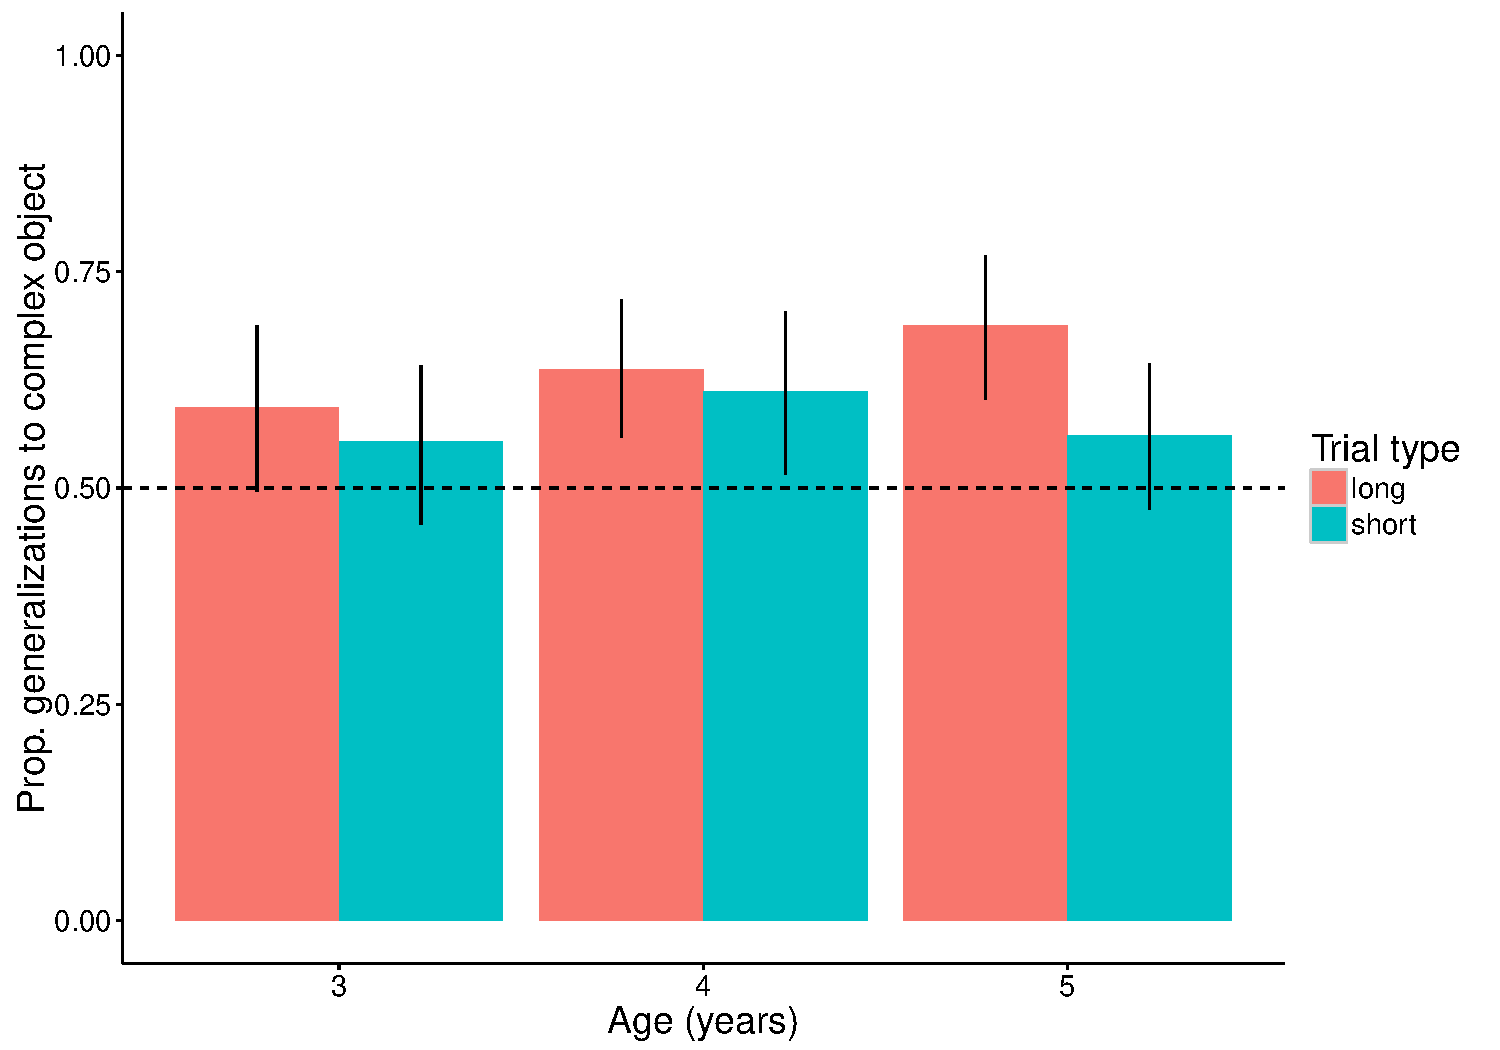
\includegraphics[scale = .5]{figs/chap4_2.pdf}
\end{center}
\caption{Mean proportion selections to complex object for children in Study 2. Error bars represent  95\% CIs as computed via non-parametric bootstrap. }
\label{fig:study2}
\end{figure*}

To test the reliability of this difference, we ran a generalized linear mixed model predicting object selection as an interaction between condition (long or short word) and age with random effects of participant and trial number. There was a main effect of age ($\beta=-0.40$, $p <.01$), indicating that children were overall more likely to select the complex  referent with increasing age. There was also a reliable interaction between age and condition ($\beta=0.38$, $p <.05$). The effect of condition was not significant.

We  ran a series of paired {\it t}-tests to examine response differences between conditions for each age group (3s, 4s, and 5s). There was a reliable difference between conditions for the 5-year-old age group ($t(35) =2.35, p<.05$, $d=.48$), but not the younger groups. 

%These results suggest that older, but not younger,
\subsection{Discussion}
These results provide some tentative evidence consistent with the Learning Hypothesis: When faced with novel words, older  preschoolers have an adult-like bias to map longer words onto more complex referents. Nevertheless, it is puzzling why the younger children in our sample, who are likely to be learning many new words, did not show the bias. This null effect may reflect a true absence of a complexity bias in young children. One possible explanation of this absence is that the bias is pragmatically driven and younger children do not have yet have competency in this type of reasoning. This possibility is consistent with a body of work on children's interpretation of scalar implicatures that suggests that reasoning in this age group is fragile and highly sensitive to aspects of the task \cite<for a review, see>{horowitz2016the-trouble}. Alternatively, this bias may simply be smaller in this population and we do not have the power to detect it in the current study. The present data do not allow us to distinguish between these two possible explanation of the null finding in the younger children.. 

Minimally, however, these data  suggest that relatively young children show a complexity bias, and thus that conceptual complexity may play a role in word learning,  as predicted by the Learning Hypothesis.

%%%%%%%%STUDY 2b - CDI%%%%%%%%
\section{Study 2b: Conceptual complexity and the early vocabulary}
In Study 2b, we explore two additional predictions of the Learning Hypothesis:  (1) Children's early vocabulary should contain a complexity bias, and (2) the conceptual complexity of a word's meaning should influence the ease with which words are learned. In particular, we predict that if conceptual complexity is relevant in acquisition, then children should tend to acquire words with simpler meanings before those with more complex meanings.

To test these predictions, we analyzed the conceptual complexity of words in children's early vocabulary using the MacArthur-Bates Communicative Development Inventory \cite<CDI;>{fenson2007}, a parent-report checklist of children's word knowledge. We find evidence consistent with both predictions: Early vocabulary contains a complexity bias, and children tend to learn conceptually simple words before more complex ones.

\subsection{Method}
\subsubsection{Participants} We recruited 252 participants from Amazon Mechanical Turk.
\subsubsection{Stimuli} Participants were presented with a subset of words from the Words and Sentences Form of the CDI \cite{fenson2007}. We excluded items that were onomatopoeic sounds (e.g.\ ``moo") or contained more than one word (e.g.\ ``rocking chair"). The final list contained 625 items. 
\subsubsection{Procedure} We used the same norming procedure as in Study 1a, except that participants were given an example of a simple and complex meaning in the instructions and  rated two anchor words (``ball" and ``motherboard;" as in Study 9 in Chapter 2). Each participant rated a sample of 40 words. 

\subsection{Results and Discussion}
The mean complexity rating for the anchor words suggested that participants  interpreted the scale as intended (``ball:" $M =1.33$; $SD = .93$; ``motherboard:" $M = 5.86$; $SD = 1.66$). Each of the 625 target words  was rated by an average of 16 participants, with a mean complexity rating of 2.77 ($SD = .77$). We next analyzed how these by-item complexity norms were related to two factors: Word length (Analysis 1; complexity bias) and age of acquisition (Analysis 2). 

\begin{figure}[t!]
\begin{center}
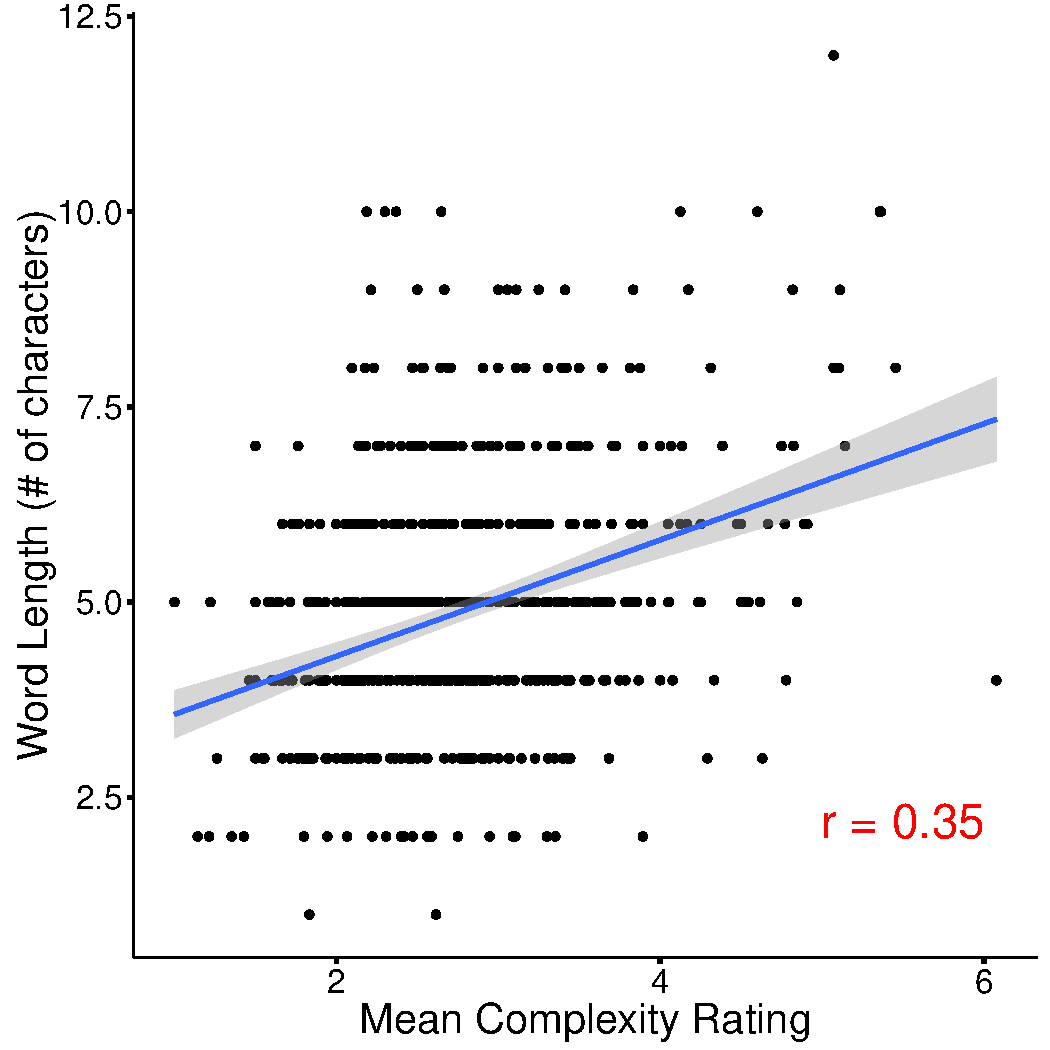
\includegraphics[scale = .5]{figs/chap4_3.pdf}
\end{center}
\caption{Word length as a function of complexity norms for all items on the CDI Words and Sentences Form. In child vocabulary, words that are conceptually more complex tend to be longer.}
\label{fig:study3}
\end{figure}


\subsubsection{Analysis 1: Complexity bias in acquisition}
As in previous studies, there was a reliable correlation between word length and complexity norms: Words whose meanings were rated as more complex tended to be longer ($r=0.35, p<.001$; Figure \ref{fig:study3}). To evaluate this relationship controlling for frequency, we fit an additive linear model predicting word length with frequency (log) and complexity. We used an existing metric of spoken word frequency derived from CHILDES, a child-directed corpus \cite{braginsky2016from}. This measure was only available for the subset of words (Words and Gestures Form; $n = 391$), and thus we only conducted this control analysis on this subset. In this analysis, both complexity ($\beta=.68$, $t=7.51$, $p <.0001$) and spoken word frequency ($\beta=-.52$, $t=-10.44$, $p <.0001$) were reliable predictors of word length, suggesting that complexity accounted for variability in word length over and above spoken frequency.

We also examined whether a complexity bias was present in acquisition cross-linguistically. We analyzed translation equivalents of the set of words on the Words and Gestures CDI form, taken from \citeA{braginsky2016from}. We analyzed  languages present in all three datasets thus far studied---the Google words (Chapter 2, Study 10), the Swadesh words (Chapter 4, Study 1), and the present set of CDI words---leaving us with a total of seven languages, including English. All seven languages showed a complexity bias. In addition, there was a positive correlation across languages between the CDI words and the Google words ($r = .30, p = .52$), and between the CDI words and the Swadesh words ($r = .59, p = .30$), though neither of these correlations were statistically significant. Figure \ref{fig:synthesis4} shows the correlation coefficient for each language, in each dataset, as well as the correlation partialing out log spoken frequency. While these data represent only a small sample of languages, they are suggestive that the bias is stable across different samples of words.

\begin{figure}[t!]
\begin{center}
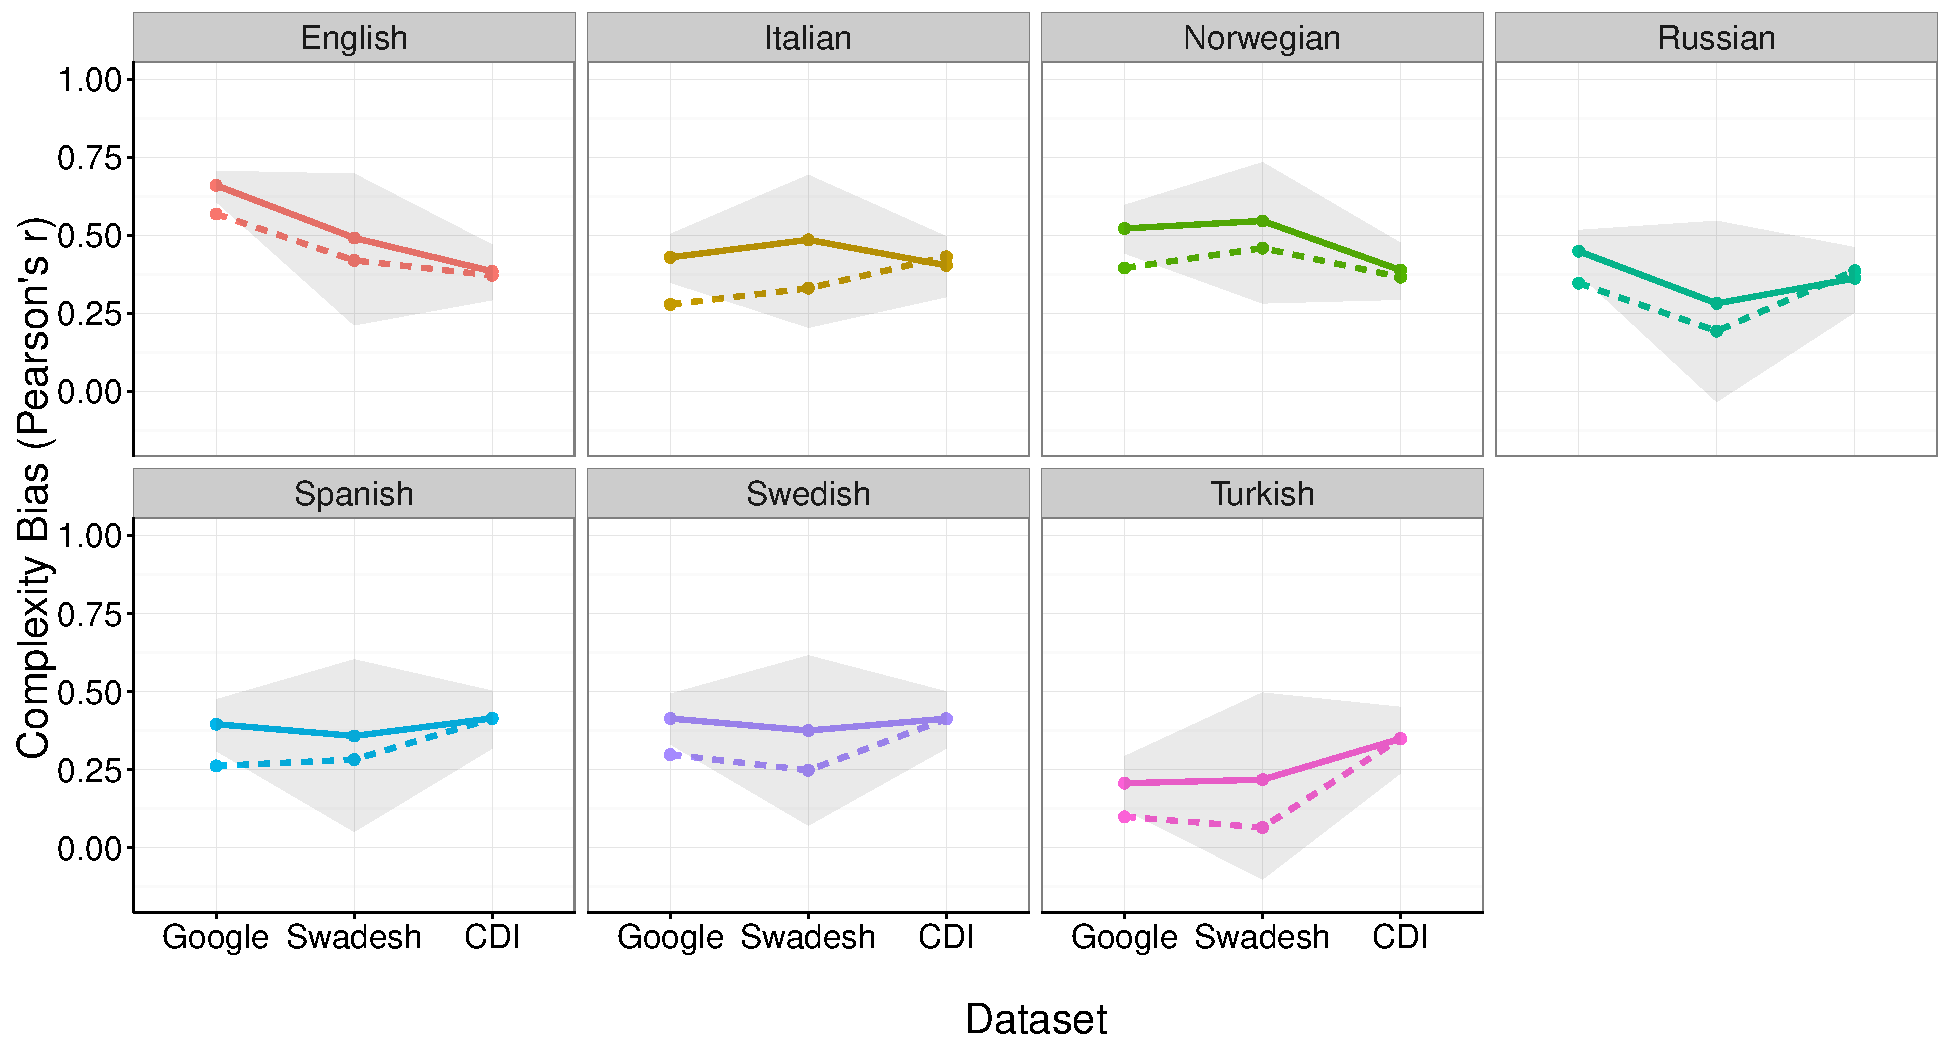
\includegraphics[scale = .47]{figs/chap4_synthesis2.pdf}
\end{center}
\caption{Pearson coefficients between word length and complexity norms across three samples of words (Google, Ch.\ 2, Study 10; Swadesh, Ch.\ 4, Study 1; and CDI Words and Gestures Form, Ch.\ 4, Study 2) for seven different languages. Solid lines show simple correlation between word length and complexity, and dashed lines show the correlation partialing out the effect of log spoken frequency. Ribbons show the parametric 95\% CI for the simple correlation. }
\label{fig:synthesis4}
\end{figure}




\subsubsection{Analysis 2: Conceptual complexity as a predictor of age of acquisition}
In Analysis 2, we asked whether the complexity of a word's meaning predicted its age of production. We estimated the age of acquisition of a word using the measures from \citeA{braginsky2016from}. In this work, age of acquisition for each word is estimated based on a database of CDI parent-report vocabulary forms  from over 42,000 children \cite<Wordbank;>{frank2016wordbank}. Using this database, \citeA{braginsky2016from} estimated the age of acquisition of each word as the age at which at least 50\% of children produce the word. In the present analysis, we find a reliable correlation between mean age of production of a word and conceptual complexity ($r=.20, p<.0001$; Figure \ref{fig:study3aoa}): Words that are conceptually more complex tend to be produced later in development. 

\begin{figure}[t!]
\begin{center}
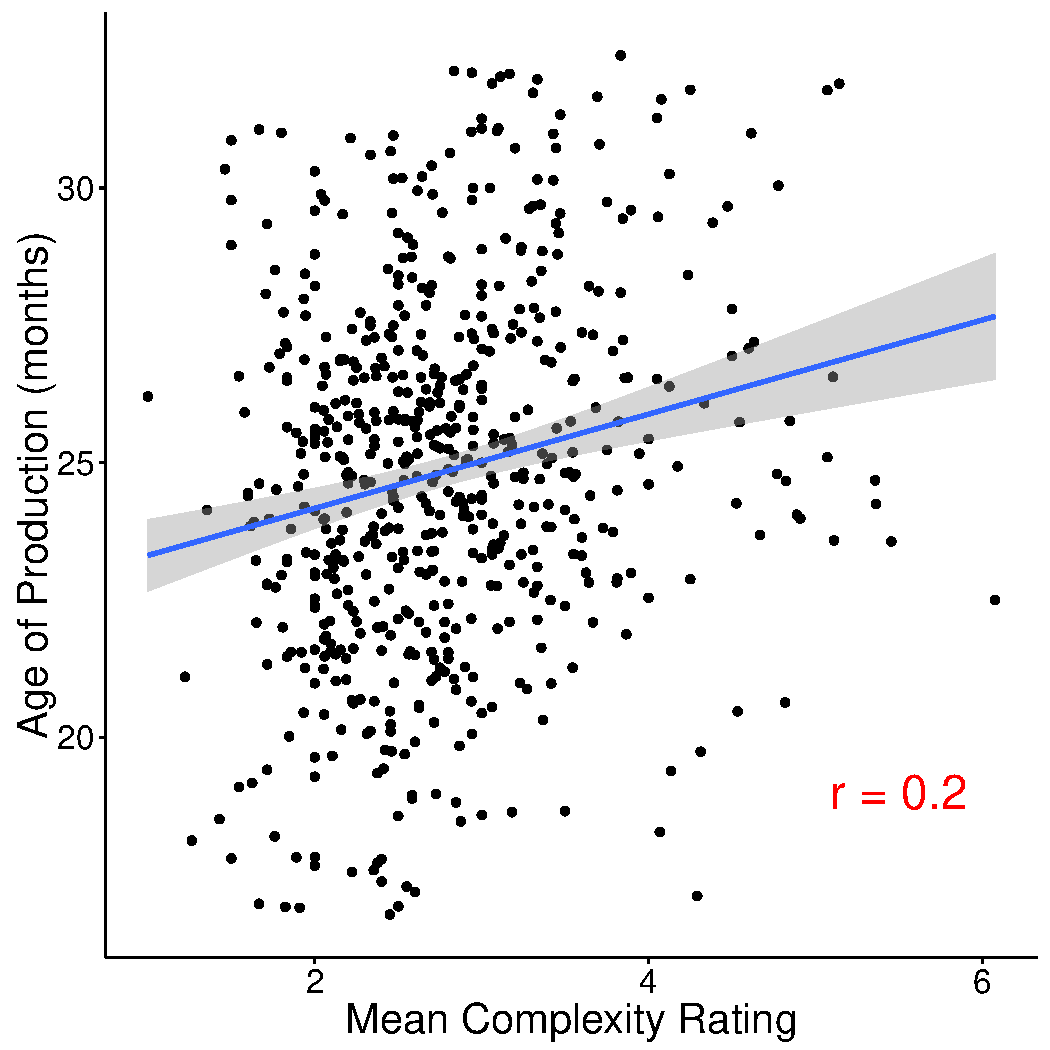
\includegraphics[scale = .5]{figs/chap4_aoa.pdf}
\end{center}
\caption{Age of production as a function of conceptual complexity. Words that are conceptually more complex are produced later.}
\label{fig:study3aoa}
\end{figure}





Importantly, however, the age of acquisition of a word is predicted by many other factors, such as the length of the word itself. Thus, we next asked whether complexity is an independent predictor of variance in the age of acquisition of words. We fit an additive linear model predicting age of production of each word with complexity, and six control variables from \citeA{braginsky2016from}: Word length, spoken frequency, concreteness (abstract vs.\ concrete), babiness (degree of association with infancy), valence (happy vs.\ unhappy), and arousal (excited vs.\ calm).  Again, these control variables were only available for the subset of words on the Words and Gestures Form ($n = 391$), and so we conducted the control analysis only on this subset. All variables were reliable predictors of age of acquisition, except word length and valence. Model fits are shown in Table \ref{tab:aoapred}. This suggests that the complexity of a word's meaning many influence the ease with which a word is acquired in language production: More complex words are produced later.

% latex table generated in R 3.3.0 by xtable 1.8-2 package
% Wed Oct 26 11:31:00 2016
\begin{table}[t!]
\centering
\begin{tabular}{rrrrr}
  \hline
 & Estimate & Std. Error & t-value & p\\ 
  \hline
(Intercept) & 8.7866 & 2.0437 & 4.30 & $<.0001$ \\ 
  complexity & 0.5154 & 0.2552 & 2.02 & $<.05$ \\ 
  word length & -0.1626 & 0.1450 & -1.12 & 0.26\\ 
  log frequency  & -1.2439 & 0.1801 & -6.91 & $<.0001$ \\ 
  concreteness & -1.0974 & 0.2502 & -4.39 & $<.0001$\\ 
  babiness & -0.4313 & 0.0864 & -4.99 &$<.0001$\\ 
  valence & 0.2037 & 0.1587 & 1.28 & 0.20 \\ 
  arousal & 0.4159 & 0.2037 & 2.04 &$ <.05$ \\ 
   \hline
\end{tabular}
\caption{Additive linear model predicting age of production of a word with conceptual complexity, and six other control variables. Complexity is a reliable predictor of age of acquisition}
  \label{tab:aoapred}
\end{table}

In summary, in acquisition we find that (1) older preschoolers have an in-the-moment complexity bias, (2) children's early vocabulary shows a complexity bias across seven different langauges, and (3) complexity predicts the age of acquisition of new words. Taken together, these findings are consistent with the possibility that the  complexity bias observed in natural language may be influenced by a learning bias in children over the course of language acquisition, as predicted by the Learning Hypothesis. 


%%%%%%%%STUDY 3%%%%%%%%
\section{Study 3: Iterated learning in a solo memory task}

In Study 3, we directly explore the Memory Hypothesis as a possible explanation of the origin of the complexity bias in natural language. The Memory Hypothesis posits that speakers mis-remember word forms in a way that is consistent with a complexity bias (shorten simple forms and lengthen complex forms) and, over time, these errors influence the structure of the lexicon.  To test this hypothesis, we use the iterated learning paradigm, a recently-developed method for studying language change in the lab \cite<e.g.,>{kirby2008cumulative,reali2009evolution,smith2010eliminating}. The critical feature of this paradigm is that the learning output of one speaker becomes the learning input for a new speaker. This paradigm allows us to examine the evolution of a language for a ``chain'' of speakers learning and transmitting a language. The dynamics of these chains serve as an approximation of the dynamics of generations of children acquiring and then transmitting language to future generations. 



A secondary goal of this study is to examine how psychological pressures influence the structure of the lexicon, independent of conceptual pressures.  Forms that are difficult to remember are unlikely to survive in the language  \cite{christiansen2008}, and there may be an additional communicative pressure for economy of expression \cite{zipf1949human}. Both of these pressures might lead to a preference for shorter words over longer, harder-to-produce words, biasing the ultimate structure of the lexicon towards shorter, more memorable words. 

We used an iterated learning paradigm to study the dynamics of these two aspects of the lexicon: how  words change over the course of language evolution and how conceptual complexity interacts with these changes.\footnote{For ease of measurement, we operationalize word length in terms of number of orthographic characters. However, this measure is highly correlated with measures of length with greater psychological reality, such as phonemes and morphemes (see Chapter 2).} As predicted, we find that forms in the lexicon converge to a more stable state and that a complexity bias emerges in the mappings between words and referents. We also find that the complexity bias is attenuated over time. A post-hoc analysis suggests that this change in the complexity bias over time is related to the degree of cross-generational change in the lexicon.


\subsection{Method}

Given existing evidence that a complexity bias is present in one-shot learning games (Chapter 2),  our experiment was designed to test how conceptual pressures influenced the lexicon over the course of transmission. We asked speakers to learn a novel language that contained meanings of varying complexity and words of varying length. Critically, the language we asked participants to learn contained no systematic relationship between complexity and word length. After studying these mappings, participants were asked to recall them. The measure of interest was the relationship between the errors participants made and the complexity of the referent. If participants show a complexity bias, they should be more likely to add characters for more complex objects and remove characters for less complex objects. 

This design characterized the first generation of our task. We then gave the labels that participants produced in the test phase of this first generation to a new set of speakers and asked them to complete the exact same task. We iterated 7 generations of this task in total.


\subsubsection{Participants} 

We recruited 350 participants from Amazon Mechanical Turk. Each generation was composed of 50 learners.

\subsubsection{Stimuli}

The referents were a set of 60 real objects that did not have common labels associated with them. These objects had been normed for their complexity in previous work (Study 4, Chapter 2; Fig.\ \ref{novelrealobjs}). Norms were obtained by asking participants to indicate ``How complicated is this object?" using a slider scale. Norms were highly reliable across two samples of 60 participants. Based on these norms, we divided the objects into quintiles of 12 objects each. Each participant saw 2 objects from each quintile. 
%\squeezeup

%\begin{figure}[b!]
%\begin{center}
%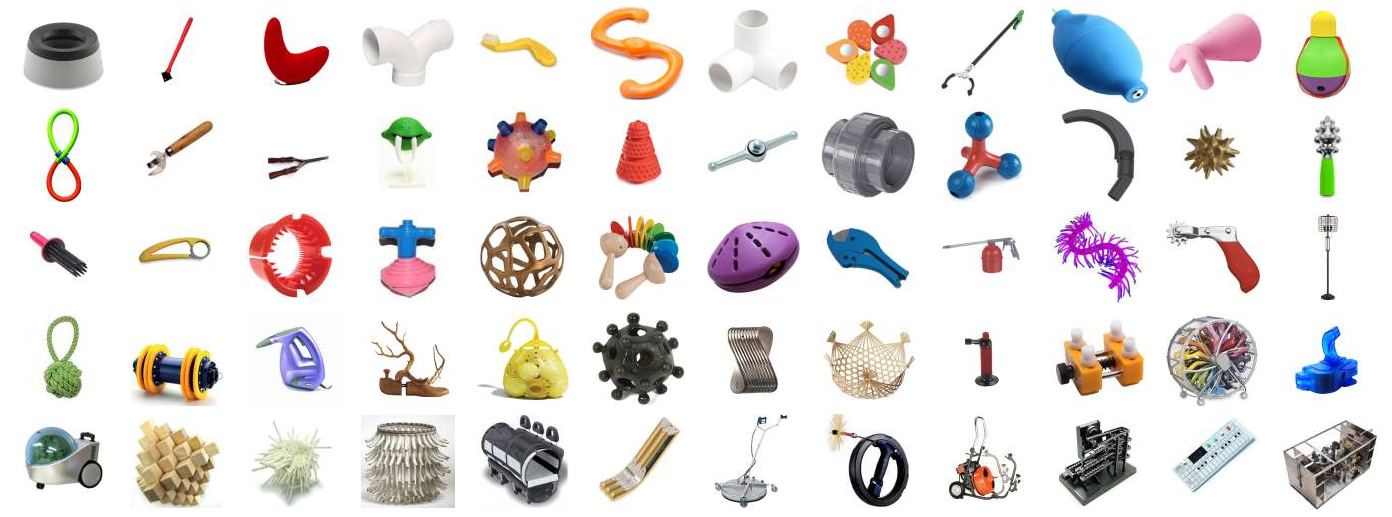
\includegraphics[width = 1\linewidth]{figs/realobjs.pdf}
%\end{center}
%\vspace{-.24em}
%\caption{Object stimuli used in the Experiment. The objects are sorted from least complex (top left) to most complex (bottom right) based on the complexity norms in Chapter 2. Each row corresponds to a quintile.}
%\label{fig:objs}
%\vspace{-1em}
%\end{figure}



In the first generation, the words were composed of randomly concatenated syllables of 3, 5, 7, 9 or 11 characters in length. Words contained CV syllables and ended in a consonant (e.g., ``gan," ``panur," ``pugimog," ``tigadogog," and ``mogonokigan"). Each participant saw 2 words of each length. The assignment of word lengths to objects was arbitrary.

Participants in Generation 2 were yoked with a participant from this first generation. This meant a participant in Generation 2 would see the exact same set of pictures as the yoked participant from Generation 1, but would learn the labels for those objects that the yoked participant had produced in the testing phase of Generation 1. Order of presentation in the training phase was randomized across generations. We iterated this procedure for a total of 7 generations.

\subsubsection{Procedure} 


Participants viewed a webpage that informed them they would be learning the names of 10 objects in an alien language. They were told they would see the names for each object four times and then their memory for the name of each object would be tested. Participants next viewed a screen displaying an object and the associated label below it. Participants pressed the space bar to advance to the next picture. Each picture-word pair was shown four times. 

In the test phase, participants saw a screen with a picture and were asked to type the learned label in a text box below the picture. Memory for each of the 10 objects was tested.

\subsection{Results}



We conducted three analyses exploring how iterated learning influenced the structure of lexicons.\footnote{All code and data for the paper are available at \url{http://github.com/mllewis/iteratedRC}.} In Analysis 1, we examined the evolution of lexical forms. In Analysis  2, we considered the relationship between word length and referent complexity. This was the key analysis because it allowed us to test for a complexity bias in the lexicon and how this bias changed over time. Finally, in Analysis  3, we conducted a post-hoc analysis to understand the source of variability in cross-generational change in complexity bias across chains.


% latex table generated in R 3.1.0 by xtable 1.7-4 package
% Fri Jan 23 11:41:41 2015
\begin{table*}[t]
\centering
%\begin{tabular}{r|llllllllll}
%\begin{tabular}{r| |l | l |l |l |l|l |l |l|l| l}
\begin{tabular}{c rrrrrr}
\hline
 %\multicolumn{11}{c}{Object} 
 %\hline

% \rule{0pt}{2ex}    
& 1 (Q1)  & 2 (Q2) & 3 (Q3) &4 (Q4) &  5 (Q5)  \\ 
 \hline
    {\it Gen.\ 0} & damitobup & nid & dunobax &  bipag &  nimimog \\ 
   {\it Gen.\ 1}& nilobup & nid & dunobug& bipag  & nimimog \\ 
    {\it Gen.\ 2} & nilobup & nid &  dunbug & bippenbog &  nimobop  \\ 
  {\it Gen.\ 3} & nilobop & nid & rdabop &  buttenbug &  nimobop \\ 
   {\it Gen.\ 4} & nilobop & nid &  dabop & buttenbop &  nimbobop \\ 
    {\it Gen.\ 5}  & nilop & nir &  dabop &  bittenbop  & nilobop \\ 
   {\it Gen.\ 6}& nilop & nir & dabop &  bittenbop &nilop \\
   {\it Gen.\ 7}& nilop &  hir &  dabog &  bittenbop &nilop  \\ 
\hline
\end{tabular}
\caption{A representative language chain. Words are presented for a sample of 5 objects across 7 generations and the initial input language. The complexity quintile of the object is noted parenthetically. Across generations, words tend to get shorter, less unique, and phonotactically more probable. Words also become more likely to be remembered accurately.}
\label{tab:ex}
\end{table*}
\normalsize

\begin{figure}[t!]
\begin{center}
\includegraphics[scale = .3]{figs/Plot1.pdf}
\end{center}
\vspace{-.5em}
\caption{Changes in lexical features across generations. Error bars represent 95\% confidence intervals computed via non-parametric bootstrap across chains.}
\label{fig:length}
\vspace{-1em}
\end{figure}





Across generations, 1\% of object labels were excluded because they contained more than one word or no word was produced. In these cases, the object was re-assigned a label from a different participant in that generation. The label was selected from a trial that had both the same initial word length and an object from the same quintile. 

\subsubsection{Analysis 1: Word forms}



Table \ref{tab:ex} presents a representative language chain. We analyzed four features of the lexical forms, averaging across each of the 50 chains at each generation: mean word length, number of unique words, transition probability, and accuracy. We also analyzed the degree of lexical change at each generation using the Levenshtein edit distance metric.

Across generations, mean word length decreased from an initial length of 7 characters to 5.22 characters in Generation 7 ($SD= 2.25$; $r=-0.22, p<.0001$; Figure\ \ref{fig:length}a). The number of unique words also decreased across generations ($r=-0.35, p<.0001$; Figure\ \ref{fig:length}b). Lexicons tended to reduce in size by mapping the same word to multiple objects (e.g.,\ in the chain presented in Table \ref{tab:ex}, ``nilop'' refers to both Objects 1 and 9).




Third, the mean orthographic transition probability of each word increased across generations ($r=.52, p<.0001$; Figure\ \ref{fig:length}c). Transition probabilities were calculated based on the set of words in the lexicon for a particular participant at a particular generation. This finding suggests that lexicons became more phonotactically structured across time. We also calculated the mean transition probability of each word using English transitions. Probabilities were estimated via orthographic bigrams from the Google Books corpus \cite{norvig}. In this analysis, the mean English transition probability of each word also increased across generations ($r=0.18$, $p <.001$), suggesting that the orthographic structure of individual words became somewhat more similar to English across generations. % vowel/consonants


Fourth, we found that participants became more accurate in recall across generations ($r=.46, p<.0001$; Figure\ \ref{fig:length}d). To examine the relationship between accuracy and word forms, we constructed a logistic mixed-effects model predicting accuracy with word length, word uniqueness, and transition probability.\footnote{The model specification was as follows: \texttt{accuracy $\sim$ guessed label length~$\times$~transition probability~$\times$~ uniqueness + (guessed label length~\textbar~subject) +  (1~\textbar~chain)}.} Only word length was a reliable predictor of accuracy ($\beta=1.21$, $p <.0001$), suggesting that perhaps the increase in accuracy across generations was due to the shorter length of the words in these languages. %phonotactics is highly collinear with number of unique words so can't put in both predictors [f

\begin{figure}[t!]
\begin{center}
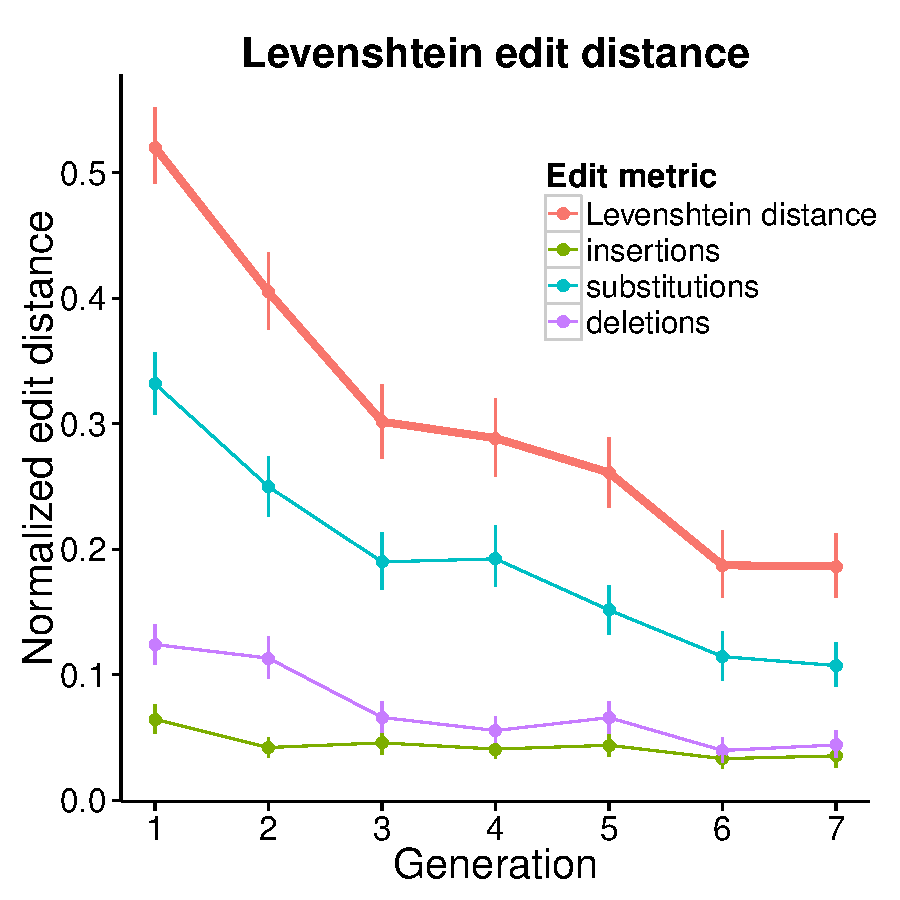
\includegraphics[width = .6\linewidth]{figs/lev.pdf}
\end{center}
\caption{Edit distance across generations, normalized by length of the longest word (guessed word vs.\ actual word). The top line shows the Levenshtein edit distance. The lines below reflect the components of this metric (substitutions, deletions, and insertions). Error bars represent 95\% confidence intervals computed via non-parametric bootstrap across chains. Number of edits decreased across generations.}
\label{fig:lev}
\end{figure}



%To examine the relationship between accuracy and features of the lexical forms, we constructed an additive linear model predicting accuracy with word length, number of unique words, and mean bigram probability. Both word length ($\beta=-0.25$, $p <.0001$) and number of unique words ($\beta=-0.28$, $p <.0001$) were reliable predictors of accuracy. This suggests that the increase in accuracy across generations was related to these changes in the features of the lexicon.

Finally, we analyzed word changes across generations using Levenshtein edit distance. This measure provides a formal metric of the similarity between two strings. Levenshtein edit distance is computed by counting the minimum number of character edits necessary to transform one word into another. For example, the edit distance from ``can" to ``cat" is 1 (1 substitution), while the edit distance from ``can" to ``calculator" is 8 (1 substitution and 7 insertions). For each word, we calculated a normalized measure by dividing the edit distance between the guessed word and the actual word by the length of the longest of the two. This normalized measure controlled for the decrease in word length across generations.  Across generations, the normalized edit distance decreased ($r=-.30, p<.0001$; Figure\ \ref{fig:lev}). This decreasing trend also held for each of the components of the Levenshtein metric: number of deletions ($r=-.18, p<.0001$), insertions ($r=-.08, p<.0001$) and substitutions ($r=-.27, p<.0001$). 

Taken together, this set of analyses points to a lexicon that is evolving to become more regular and consequently easier to learn.


%consonant/vowel analysis?

\subsubsection{Analysis 2: Complexity bias} 

In Analysis  2, we examined the relationship between changes in word length and the complexity of referents. If there is a complexity bias in the lexicon, participants should be more likely to produce longer labels for more complex referents. 

We considered two metrics of word length: Label length in characters and cumulative characters removed (CCR). CCR is calculated by subtracting the word length at a particular generation from the input generation word length. Though slightly more complex, CCR provides a length metric that controls for variability in input word length; this control is important because words varied dramatically in their initial length due to random assignment in the initial generation. We calculated $p$-values based on an empirical distribution of $r$-values, obtained by sampling from random pairings of words and objects. This was done because changes in  language forms across generations change the distribution of possible $r$-values.

\begin{figure}[t!]
\begin{center}
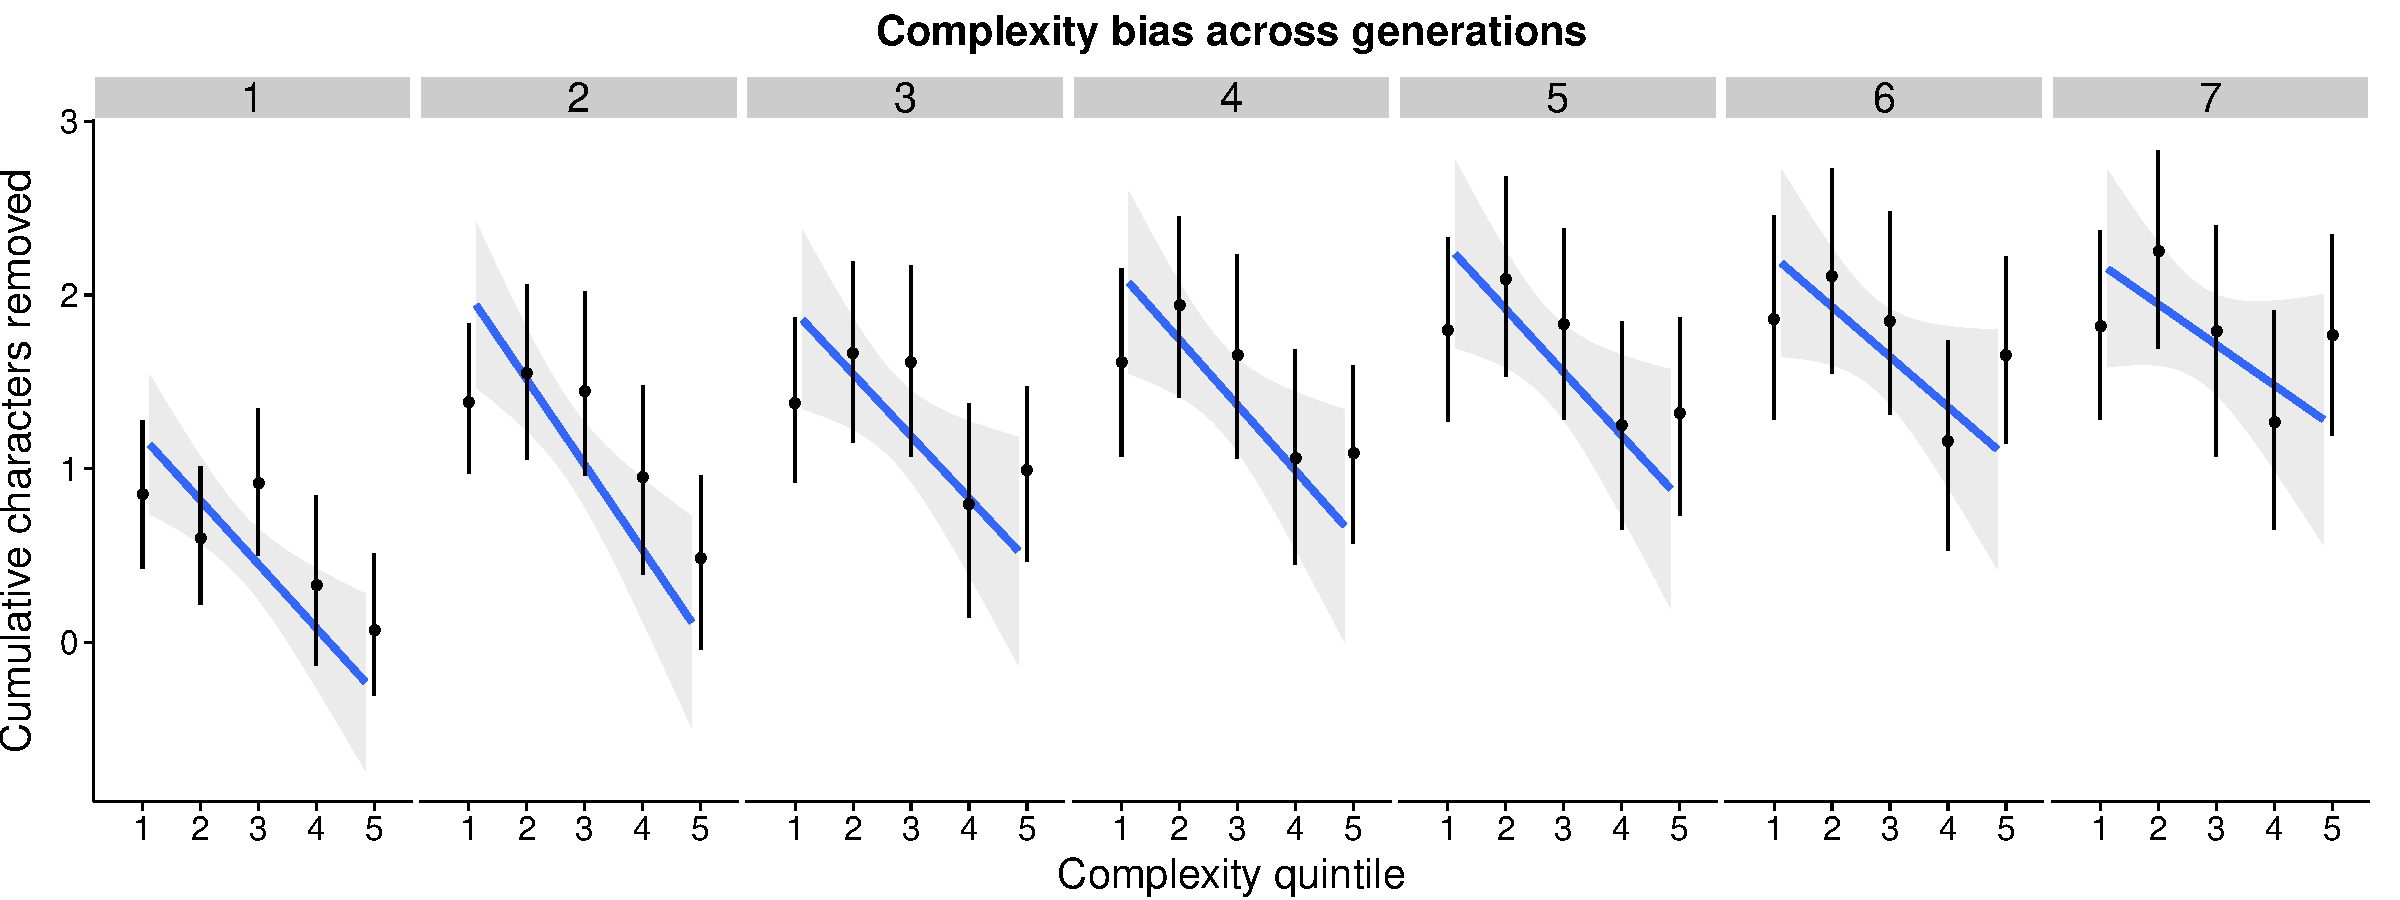
\includegraphics[scale = .38]{figs/complexity_bias.pdf}
\end{center}

\caption{Cumulative characters removed as a function of complexity across all 7 generations. Points correspond to the quintile means. Lines represent the best fitting linear model predicting word length from the complexity norm of the object. Negative slopes indicate a bias to recall longer labels for  more complex objects. Across generations, this bias decreased.}
\label{fig:cbias}
\end{figure}



Across generations, there was a reliable bias to map longer words to more complex referents across both measures of length (label length: $r=.05, p<.05$; CCR: $r=-.11, p<.0001$). Figure \ref{fig:cbias} shows CCR as a function of object complexity across generations. Qualitatively, the bias decreased across generations. However, there was high variability across chains both in the total complexity bias (label length: $SD = .27$), and in how this bias changed across generations (label length: $M = .004$; $SD = .69$).

\begin{table}[t!]

\centering
\begin{tabular}{cc|ccccccc}

\multicolumn{2}{c}{\multirow{2}{*}{}} & \multicolumn{4}{c}{Quintile  1}\\
\multicolumn{2}{c|}{}                    & 2 & 3 & 4 & 5\\ \cline{2-6}
\multirow{4}{*}{\rotatebox{90}{Quintile  2}} & 1 & 86 &  78 & 64 & 52 \\
                                      & 2 &    &   84 & 63 & 34\\
                                      & 3 &   & & 41 & 59\\
                                       & 4 &   &  &  & 58\\
                                       \vspace{-.5em}

\end{tabular}  

\caption{Contingency table of trials where participants recalled the same word for multiple objects. Columns correspond to the complexity quintile of the target object and rows correspond to the  complexity quintile of the object with the same word. The diagonal is excluded because the experimental design restricted the number of possible confusions for these cases (1 possible alternative vs.\ 2 for all other quintiles). In cases of confusions, participants tended to reuse a word from an object in a nearby quintile.}
\label{tab:confusion}
\end{table}

A number of other exploratory analyses suggest a role for complexity in language change. First, Levenshtein edit distance was systematically related to the complexity of referents: Participants were more likely to edit words referring to more complex referents ($r=.05, p<.01$). Second, there was systematicity in the kinds of errors participants  made when reusing words across multiple objects. Participants tended to reuse labels from objects of nearby quintiles (Table\ \ref{tab:confusion}), suggesting that these labels were more conceptually confusable and lead to more category-formation.

Together, this set of analyses replicates prior work suggesting a complexity bias in the lexicon: Across both measures of word length, participants tended to recall longer labels to refer to more complex referents. They were also more likely to edit words related to more complex referents and reuse labels of objects from nearby quintiles. However, an unexpected finding was the attenuation of this bias across generations. In our last analysis, we try to understand this trend.

%\begin{figure}[t]
%\begin{center}
%\includegraphics[scale = .4]{figs/confusion.pdf}
%\end{center}
%\caption{Contingency table for all trials in which participants recalled the same word for multiple referents. The diagonal is excluded because the experimental design restricted the number of possible confusions for these cases (1 possible alternative vs.\ 2 for all other quintiles). When a participant mapped the same word to a second referent, they tended to reuse a word from an object in a nearby quintile.}
%\label{fig:confusion}
%\end{figure}
% latex table generated in R 3.1.0 by xtable 1.7-4 package
% Tue Feb  3 10:17:16 2015

  
\subsubsection{Analysis  3: Relationship between change in word forms and change in complexity bias} 


\begin{figure}[t]
\begin{center}
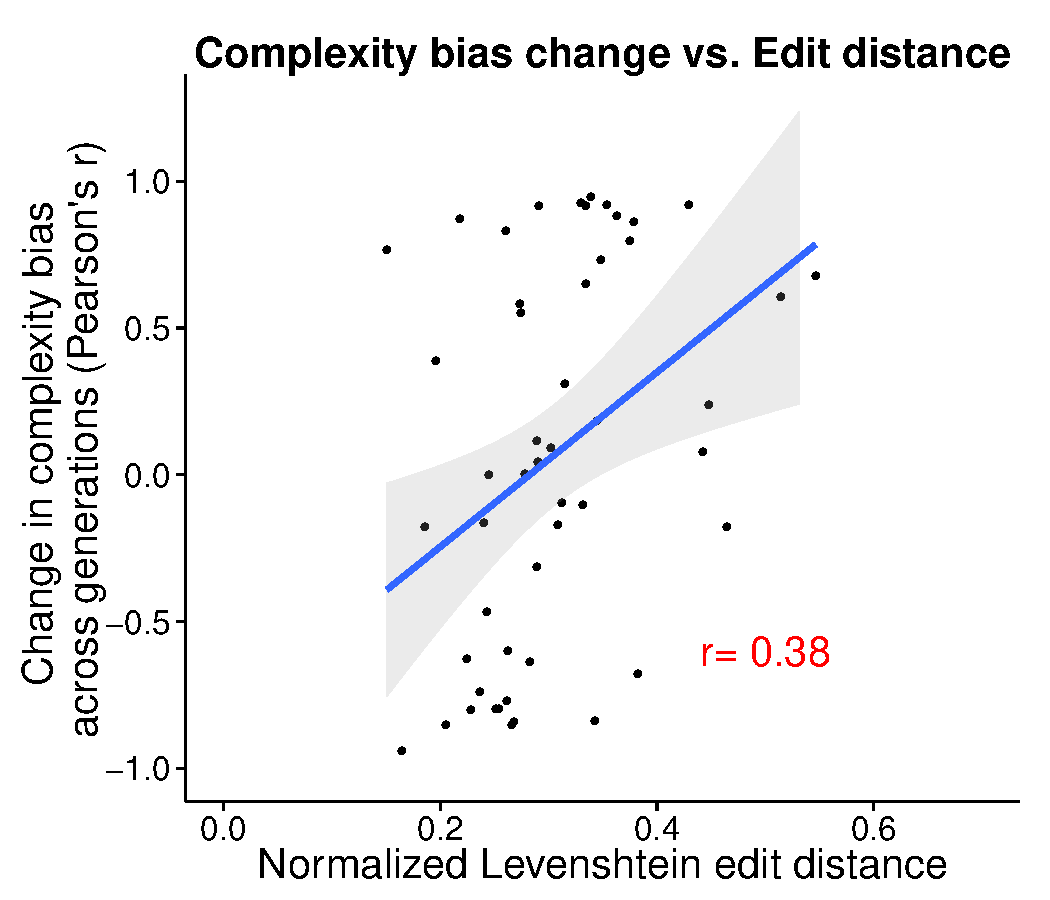
\includegraphics[width = .6\linewidth]{figs/change_plot.pdf}
\end{center}
\caption{Complexity bias as a function of the normalized Levenshtein edit distance of the chain. Complexity bias is calculated here using number of cumulative characters removed. Each point corresponds to an individual chain. Chains with greater normalized Levenshtein distances tended to show a greater increase in complexity bias across generations.}
\label{fig:levcbias}
\end{figure}



We  conducted a post-hoc exploration of the variability in the complexity bias across chains. For each chain, we quantified the complexity bias at each generation by calculating the correlation between metrics of length (label length and CCR) and the complexity norms. We then calculated the correlation between these coefficients and generation. This gave us a measure of the change in the complexity bias across generations. We considered how this change in complexity bias related to the degree of change in the forms of the lexicon. Two metrics of lexical change were analyzed: accuracy and Levenshtein edit distance. 

Chains with greater cross-generational change in lexical forms tended to show an increase in complexity bias over time. Using raw label length as the length metric, there was a reliable correlation between change in complexity bias and accuracy ($r=0.29$, $p <.05$) and between  change in complexity bias  and normalized Levenshtein edit distance ($r=-0.32$, $p =.02$). This same pattern also held for the CCR length metric (accuracy: $r=-0.37$, $p <.01$; Levenshtein: $r=0.38$, $p <.01$; Figure\ \ref{fig:levcbias}).




%%%% DISCUSSION %%%%%%
\subsection{Discussion}

In three analyses, we examined change in the structure of lexicons across generations of transmission. Analysis  1 reveals that lexical forms become simpler and more regular over time. We find that words become shorter, less unique, more phonotactically probable, and more likely to be remembered. We also find that this structure facilities memory recall: lexicons with fewer and shorter words are more likely to be remembered accurately. Analysis  2 examined the relationship between lexical forms and conceptual structure, and found that a complexity bias emerges in the lexicons. 

An unpredicted result was that the complexity bias does not strengthen across generations. Analysis  3 suggests that change in the complexity bias across generations is related to the degree of change in lexical forms in the chain: Chains with more change are more likely to show an increase in complexity bias over time. The underlying mechanism supporting this relationship is straight-forward: chains that make more errors have more opportunity to deviate from the random input mappings between words and referents. This direction of this correlation suggests that when chains do in fact deviate from these initials mappings, they do so in a systematic way. That is, they tend to deviate in a way that is more likely to map longer words onto more complex referents.

%The iterated learning paradigm provides an opportunity to examine how in-the-moment psychological pressures influence the structure of a language in aggregate, over time. We examined two aspects of this structure: lexical forms and the mappings between words and objects. We hypothesized that different psychological pressures would influence each type of structure. In the case of lexical forms, we predicted there would be a bias to simplify the language into shorter, fewer forms. In the case of word-object mappings, we predicted a bias to map longer words onto more complex meanings \cite{lewisstructure2014}. The question of interest was how these psychological pressures influenced the structure of the lexicon across generations of transmission. 

%Our findings suggest that each of these pressures may have influenced the structure of the lexicon---and critically---that they interacted with each other. 

In sum, we found both a bias to simplify the lexicon and a bias to map longer words onto more complex meanings. But these pressures appear to have pushed in opposite directions: The pressure to simplify the language leads to less variability in word length, and this reduced variability suppresses the complexity bias. If these dynamics reflect actual language evolution, however, an important question still remains---why do we in fact see a complexity bias in natural language? That is, if there is a strong pressure towards simplicity, then why does a complexity bias emerge in natural language despite this pressure? 

The Pragmatic Hypothesis suggests that this this discrepancy is due to the absence of an important feature in our task: Communication with a second interlocutor. \citeA{zipf1949human} argued that the equilibrium that emerges in the lexicon is a product of both the speaker's desire to say less and the listener's desire for a more explicit, comprehensible message. Importantly, the common desire for efficiency creates opposing pressures among interlocutors. For a speaker, the optimal solution to communication is to have a lexicon that contains a single, short word that can be used to refer to all meanings. However, for a listener, the optimal solution is to have a lexicon that maps a unique word onto every possible meaning. 

Thus, perhaps the absence of a listener pressure in our task may have lead our participants (``speakers'') to simplify the language. While our task was posed as a memory task, there was no penalty for failure to remember a form. In contrast, in a communicative task, the listener's failure to comprehend a label would have acted as an incentive for accurate reproduction, perhaps limiting the amount of compression the language would undergo.  In Study 4, we test this prediction.

%But memory limitations may also play another role in the evolution of the lexicon: by introducing variation into the representations of individual words, speakers' memory constraints allow for change. In the absence of memory constraints, speakers might simply reproduce the language as is; thus, the interaction between cognitive and communicative pressures may function to {\it facilitate} the emergence of a complexity bias. 


% However, memory limitations insert ``noise'' into the lexicon and thus create the opportunity forthe emergence and regularization of a complexity bias. 

%This synergistic relationship between memory and change is reminiscent of the ``less-is-more'' hypothesis and its descendants \cite{newport1990maturational,hudson-kam2005}, in which cognitive limitations are invoked as an important mechanism in language learning and language change. In the case of the complexity bias, these proposals make testable predictions that can be explored by extending the present paradigm into a communicative domain with varying demands on memory.
%%%%%%%%STUDY 4%%%%%%%%
\section{Study 4: Iterated learning in a communicative memory task}

%Why did the complexity bias decrease across generations? One possibility is that this discrepancy is due to the absence of an important feature in our task: communication with a second interlocutor. \citeA{horn1984} argued that the equilibrium that emerges in the lexicon is a product of both the speaker's desire to say less and the listener's desire for a more explicit, comprehensible message. Importantly, the common desire for efficiency creates opposing pressures among interlocutors. For a speaker, the optimal solution to communication is to have a lexicon that contains a single, short word that can be used to refer to all meanings. However, for a listener, the optimal solution is to have a lexicon that maps a unique word onto every possible meaning. 

%Thus, perhaps the absence of a listener pressure in our task may have lead our participants (``speakers'') to simplify the language. While our task was posed as a memory task, there was no penalty for failure to remember a form. In contrast, in a communicative task, the listener's failure to comprehend a label would have acted as an incentive for accurate reproduction, perhaps limiting the amount of compression the language would undergo. 

In Study 4 ,we adopt the paradigm from Study 3 to simulate a listener. In the Communicative Feedback, the participant is paired with a fake communicative partner who provides feedback about the guesses. We also ran a control No Feedback condition that is a near replication of Study 3. If the attenuation of the complexity bias in Study 3 is due to reduced listener demands, we expect that providing feedback will reduce  attenuation and perhaps lead to an increase in complexity bias over generations. 

\subsection{Method}

\subsubsection{Participants}
We recruited 500 participants from Amazon Mechanical Turk. Participants were randomly assigned to the No Feedback or Communicative Feedback conditions. We ran a total of  five generations with 50 participants at each generation for each condition.

\subsubsection{Stimuli}
The object and linguistic stimuli were identical to Study 3.

\subsubsection{Procedure}
The task was identical to Study 3, with the exception of the feedback. We also added a second block (where a block corresponds to a training and testing phase) so that there was greater opportunity to observe effects of the feedback. In the Communicative Feedback condition, participants were told: ``In the next part of the experiment, you will be asked to work with a partner. Your partner also learned the labels for these 10 objects. Your partner will see a display of all 10 objects. Your job is to use the words you just learned to get your partner to select one of the objects." They then were  told they were paired with another participant, and shown their screen name. After entering their response in a chat box, they received feedback from the other participant. The feedback varied as a function of the Levenshtein edit distance of the word: If the word was highly different from the target word, the  dummy-partner responded with uncertainty (``I don't know what you mean"). However, if the word was sufficiently similar (above a threshold Levenshtein value), the dummy-partner responded affirmatively (``Got it'').

\subsection{Results}

We conducted the same set of primary analyses as in Study 3: Change of word forms across generations (Analysis 1), and change in complexity bias across generations (Analysis 2). 

\subsubsection{Analysis 1: Word forms}

\begin{figure}[t!]
\begin{center}
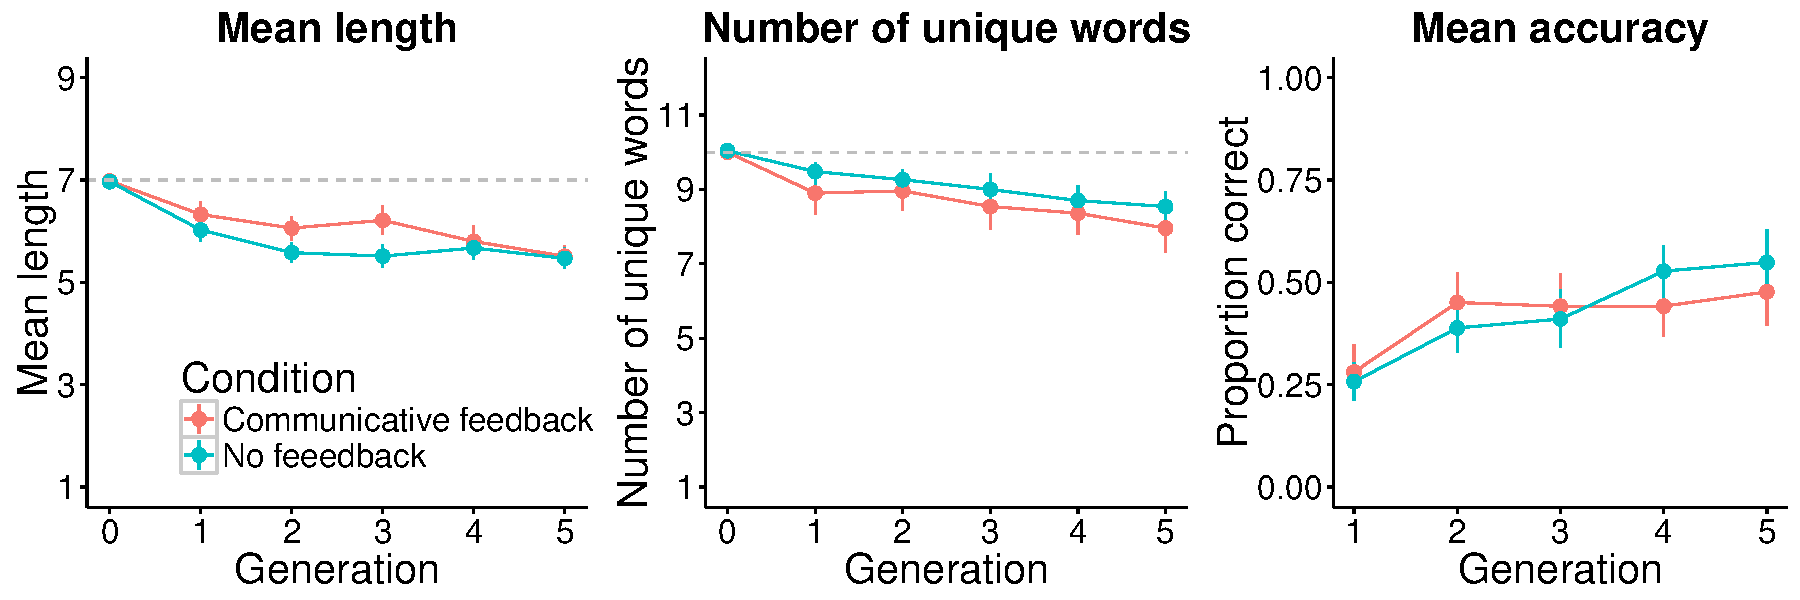
\includegraphics[scale = .5]{figs/chap4_4.pdf}
\end{center}
\caption{Changes in lexical features across generations. Error bars represent 95\% confidence intervals computed via non-parametric bootstrap across chains. }
\label{fig:length_4}
\end{figure}

As in Study 3,  mean word length and number of unique words both decreased across generations (Figure\ \ref{fig:length_4} a and b). To test for an effect of condition, we fit a mixed-effect linear model predicting word length with  condition and generation as fixed effects, and random intercepts and slopes by chain. There was a main effect of generation ($\beta=-.3$, $p <.001$). There was also an interaction with feedback condition ($\beta=-.06$, $p <.05$). This reflects the fact that word lengths decreased slower for the Communicative Feedback condition, relative to No Feedback. We then fit the same model but predicting number of unique words. There was a reliable effect of generation ($\beta=-.25$, $p <.001$), but no effect of condition.

Finally, we also found that participants became more accurate in recall across generations (Figure\ \ref{fig:length_4}c). Fitting the same model as above to predict accuracy, there was an effect of generation ($\beta=.04$, $p <.001$), and a reliable interaction between generation and condition  ($\beta=.04$, $p <.05$). This interaction reflects a small bias for participants in the Communicative Feedback condition to be more accurate in earlier generations. 

Thus, in sum, we replicate our findings from Study 3 in the No Feedback condition: Word length and number of unique words decreased across generations, while accuracy increased. In the Communicative Feedback condition, word forms decreased in length slightly slower and were initially more accurate than in the No Feedback condition. However, for the most part, we find that feedback condition did not have a substantial influence on word forms.

%However, we do not find much evidence that communicative feedback type influence the change of word forms. 
%I have run the No Feedback and Communicative Feedback condition. The No Feedback condition replicates Study 3. In the Communicative Feedback condition, mean length appears to be somewhat longer,  but the complexity bias is smaller overall and does not increase across generations.
\begin{figure}[t!]
\begin{center}
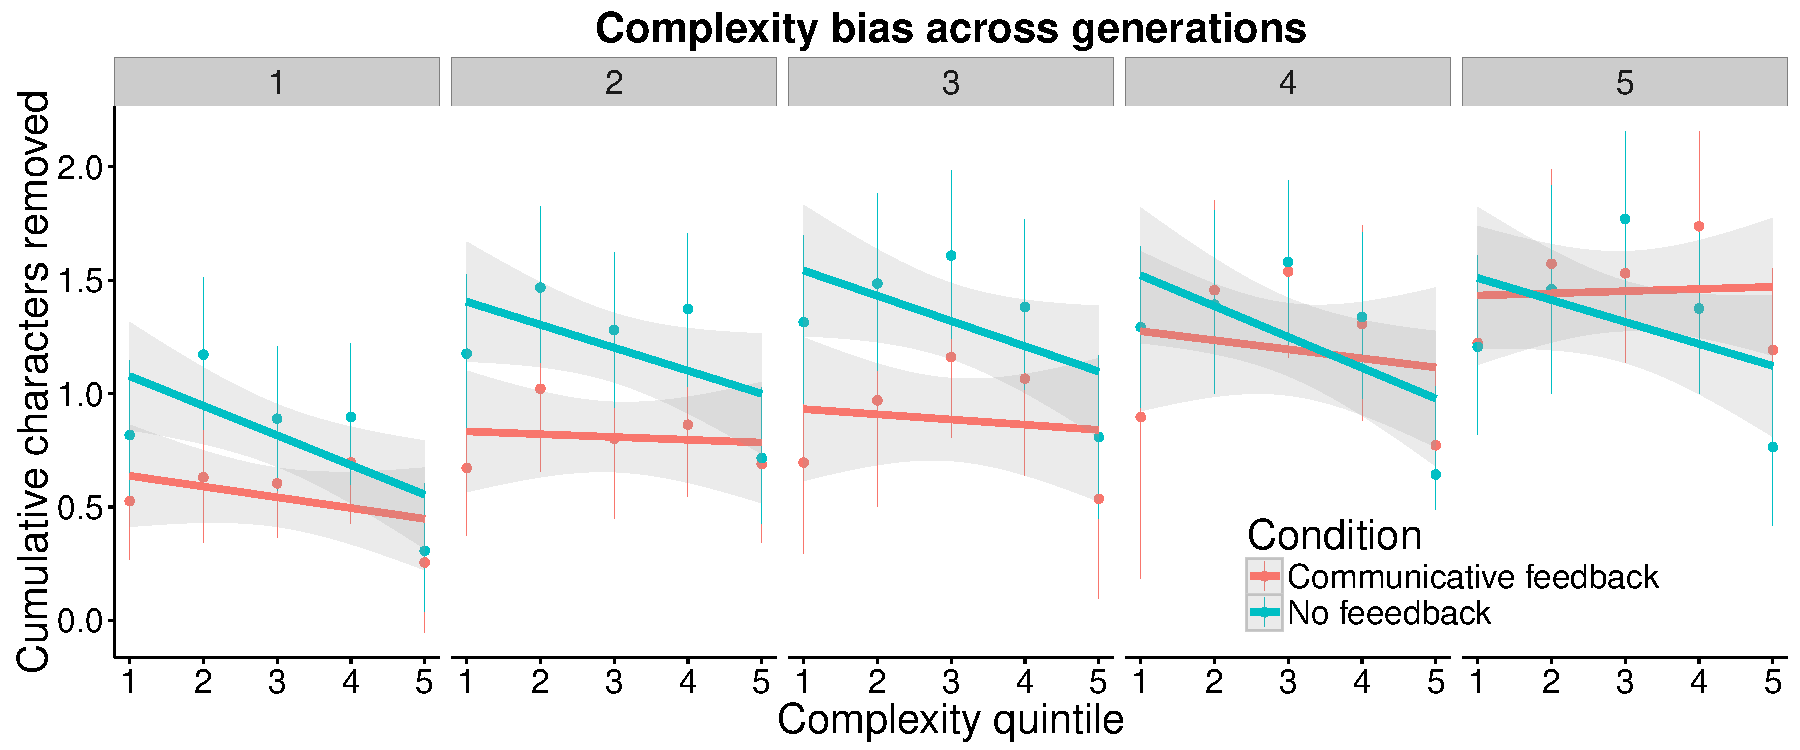
\includegraphics[scale = .5]{figs/chap4_4bias.pdf}
\end{center}
\caption{Cumulative characters removed as a function of complexity across all 5 generations. Points correspond to the quintile means. Lines represent the best fitting linear model predicting word length from the complexity norm of the object. Negative slopes indicate a bias to recall longer labels for  more complex objects. Across generations, this bias decreased, and there was no evidence to support the prediction that communicative feedback strengthened the bias.}
\label{fig:cbias4}
\end{figure}


\subsubsection{Analysis 2: Complexity bias}
In Analysis 2, we examined the key hypothesis: The magnitude of the complexity bias should be affected by feedback condition. As in Study 3, we analyzed the cumulative number of characters removed as our measure of length. For each condition, we measured the correlation between the complexity measure of the word and cumulative characters removed. Collapsing across conditions, the magnitude of the bias was larger in the No Feedback condition ($r = -0.08$), relative to the Communicative Feedback condition  ($r = -0.03$).  Figure\ \ref{fig:cbias4} shows the complexity bias across generations for each of the two conditions. Qualitatively, there is no evidence to suggest that the bias increased in the Communicative Feedback condition, as predicted by the Pragmatic Hypothesis. If anything, it appears to decrease. 

\subsection{Discussion}
The Pragmatic Hypothesis provided one possible explanation for the absence of a strengthening of the complexity bias in Study 3. In Study 4, we tested this prediction by introducing a (fake) interlocutor to give feedback to participants. However, there is no evidence to suggest that this pressure functioned to  increase the bias over time.

It is possible that this null effect is due to unusual setup of our task, such that participants did not believe the ``communicative" cover story.  A stronger test of the Pragmatic Hypothesis would therefore be to conduct the same experiment in the lab in a more realistic communicative context. Alternatively, this null effect could be because communicative pressures are not the critical pressure in decreasing word lengths in this task. The current experiment cannot distinguish between these two possibilities, but nevertheless provides some evidence against the Pragmatic Hypothesis.

\section{General Discussion }
In this chapter, we surveyed evidence relevant to four possible hypotheses about the origins of a complexity bias in natural language: The Efficient Naming Hypothesis, the Learning Hypothesis, the Memory Hypothesis, and the Pragmatic Hypothesis. In Study 1, we replicated our earlier work and found a complexity bias in a large sample of diverse languages. In Study 2, we found that children have a complexity bias in an online mapping task, and that conceptual complexity predicts the age of acquisition of a word in a child's vocabulary. In Studies 3 and 4, we found that memory errors lead to a complexity bias in an artificial language, but that this bias did not increase when a communicative partner was present.

We now have estimates of a complexity bias in natural language across three samples of words. Averaging across the seven languages described in Study 2b, we see that the magnitude of the complexity biases are remarkably comparable across a sample of seven languages, around $r = .4$ (Google: $r = .44$; Swadesh; $r = .39$;  CDI: $r = .39$). Given that all but one of these language in this subsample is from the Indo-European language family, this estimate should be interpreted cautiously. Importantly, however, we replicate our previous work pointing to a complexity bias across a range of words and languages.

Given this body of evidence, what are the most likely origins of the complexity bias in natural language? The Efficient Naming Hypothesis seems unlikely for several reasons. First, Study 1 suggests that languages have a complexity bias in a  sample of highly primitive meanings. If the Efficient Naming Hypothesis were correct, we should expect these meanings to be all assigned short words. Second, the fact that there are many unused short words in a language (e.g.\ ``dax," ``blicket," etc.) suggests that minimizing word length is not the only pressure speakers face. Indeed, there is reason to think that variability in word length is helpful for discriminating words in the cognitive system. Finally, the fact that we observe the complexity bias with novel words in word mapping tasks suggests that speakers have a cognitive representation of this bias. This cannot be explained by the Efficient Naming Hypothesis.

The evidence supporting the Pragmatic Hypothesis is also limited. In Study 4, we find no evidence that the presence of a communicative partner increased the magnitude of the bias. However, it seems possible that participants were not persuaded by the communicative cover story, though the slight difference in mean lengths across generations is some evidence against this. On the other hand, the pragmatic explanation provides a parsimonious account of children's failures in Study 1a. As has been shown in other work, young children often fail at pragmatic reasoning without sufficient contextual support. This account might then explain why the younger children in our sample, the three- and four-year-olds, failed to show a complexity bias in an online task. 

The Learning and Memory Hypotheses thus seem most likely. The fact that there is a complexity bias in children's vocabulary and that conceptual complexity predicts acquisition is suggestive that learning pressures my lead to a complexity bias in the lexicon. In addition, the fact that we see a complexity bias emerge from memory errors suggests this bias might by influenced by in-the-moment cognitive pressures. Together, these two sets of results suggest that speakers may be influenced by iconicity.

The primary focus of this chapter has been to provide an account for the complexity bias present in natural language, but a related datum is the complexity bias observed in-the-moment of language use in novel word mapping tasks. Findings from these experiments suggest that the bias is not only present in language, but is also represented in the minds of speakers and is productive. The most parsimonious account of both data points---the complexity bias in natural language and the complexity bias in novel word mapping tasks---would appeal to the same mechanism. If the Learning and Memory Hypotheses are correct, this is might mean that participants in the online mapping task are relying on the principle of iconicity to guess the meaning of the word. 

However, this need not necessarily be the case: The in-the-moment bias in the novel word mapping task could be the product of a generalization from the bias in natural language. This is a difficult possibility to explore, but one prediction of this hypothesis is that the bias should get larger as children learn more words and thus have greater evidence and certainty about the bias in natural language. The fact that the bias appears to get larger with development in Study 2a is some evidence in support of this possibility. Alternatively, the Learning and Memory Hypotheses could be the correct explanation for the bias in natural language, but participants could  be relying on pragmatic reasoning in the novel word mapping tasks.  While less parsimonious than the other accounts, this alternative is nonetheless consistent with the current body of evidence.

In conclusion, on the basis of these four studies, the most likely accounts of the complexity bias in natural language are the Learning and Memory Hypotheses: Children are biased to learn words consistent with a complexity bias, and speakers make memory errors consistent with a complexity bias. Over time, these pressures at shorter timescales lead to a bias in natural language at the language evolution timescale. The Pragmatic Hypothesis remains possible, though less likely, and more realistic communicative contexts are necessary to  definitely rule out this hypothesis.

%About .27 vs. .48



%An open question from this work is where an in-the-moment bias might originate from. Parsimony.
%
%talk about in the moment bias  lexical bias vs. (e.g. overhyopthesis, compare effect sizes) - again, not mutually exclusive, parsimony

%\subsection{naming hypothesis}
%Under this hypothesis, there are several ways to account for a pragmatic in-the-moment complexity bias. One possibility is that the lexical bias and the in-the-moment bias are the result of independent causal processes: the lexical bias may be the result of an efficient naming strategy, while the in-the-moment complexity bias may be the product of  general pragmatic reasoning. 

%An alternative possibility is that  the  in-the-moment bias emerged from a generalization, or overhypothesis \cite{kemp2007}, based on observations about the lexicon. That is, given experience with a lexicon that contains a regularity to map longer words to more complex meanings, learners might have induced a complexity  regularity about the lexicon. Thus, when faced with a novel word, speakers might apply this bias as a probabilistic heuristic about the meaning of the word. An overhypothesis account of the behavioral data has the advantage that it is able to account for the development  in an in-the-moment complexity bias in preschoolers. Under this account, preschoolers might not show this behavioral bias because they have not yet observed enough data to induce a complexity overhypothesis.




%!TEX root = ../dissertation.tex

\chapter{Pressures shaping the evolution of the lexicon}
\label{chapter:pressures}

%%%%% INTRODUCTION %%%%%%
\section{Introduction}
What factors shape language?  Psychologists have made significant progress understanding this question in the domains of communicative interaction and children's developmental trajectories. In both cases, accounts rely on positing two pressures on the cognitive system---one internal and one external. In the case of communication, theorists argue that speakers are influenced by cognitive constraints (minimize effort) and by the needs of the communicative partner \cite<be understandable;>{horn1984}. In the case of acquisition, there are internal maturational constraints, as well as external pressures from the quality and quantity of linguistic input \cite{hart1995meaningful}. In the present paper, we explore the possibility that the same two pressures---system internal and external---may also shape {\it language systems} over the course of language evolution.\footnote{This chapter is published in Lewis, M. \& Frank, M. C. (2016). Linguistic niches emerge from pressures at multiple timescales. Proceedings of the 38th Annual Meeting of the Cognitive Science Society. Austin, TX: Cognitive Science Society.}

Central to this hypothesis is the notion of a timescale: there are different units of time over which processes operate, and processes at shorter timescales influence those at longer timescales \cite[see also Figure 5.1]{blythe2015hierarchy}. At the shortest timescale  are  individual utterances in communicative interactions (pragmatics). At a longer timescale is language acquisition.  Both experimental and modeling work suggest that communicative interactions at the pragmatic timescale influence processes like word learning at the acquisition timescale \cite<e.g.,>{baldwin1991infants,mcmurray2012,frank2009a,frank2014inferring}.
%Critically, at both of these timescales, both internal and external pressures are thought to influence language (Fig. 1). 



In addition to pragmatics and acquisition, a third relevant timescale is language evolution: the timescale over which entire language systems change.   As for acquisition, there is evidence that language systems may be the product of processes at the pragmatic timescale. For example, languages universally structure semantic space to reflect optimal equilibria between communicative pressures  \cite<e.g.,>{kemp2012kinship,regier2007color,baddeley2009}.

%language evolution timescale, the goal is to explain variability at the level of language systems (Modern English vs.\ Old English; English vs.\ Thai).

However, the presence of communicative pressures at the pragmatic timescale is unable to explain cross-linguistic variability in linguistic structure. That is, why does Polish have rich morphology but English relatively sparse? A growing body of work argues that this variability may be due to cognitive constraints internal to the language learner \cite{chater2010language} as well as properties of the environmental context \cite{nettle2012social}. This hypothesis, termed the  {\it Linguistic Niche Hypothesis} \cite{lupyan2010language,wray2007consequences}, suggests that language systems adapt to the internal and external pressures of  the linguistic environment. %These pressures may come from external pressures, such as contact with other languages, as well as constraints by learners themselves. 

%from a range of sources, including the climate, the length of the growing season, or the demographic characteristics of the people who learn and speak the language. 
\begin{figure}[t!]
\begin{center}
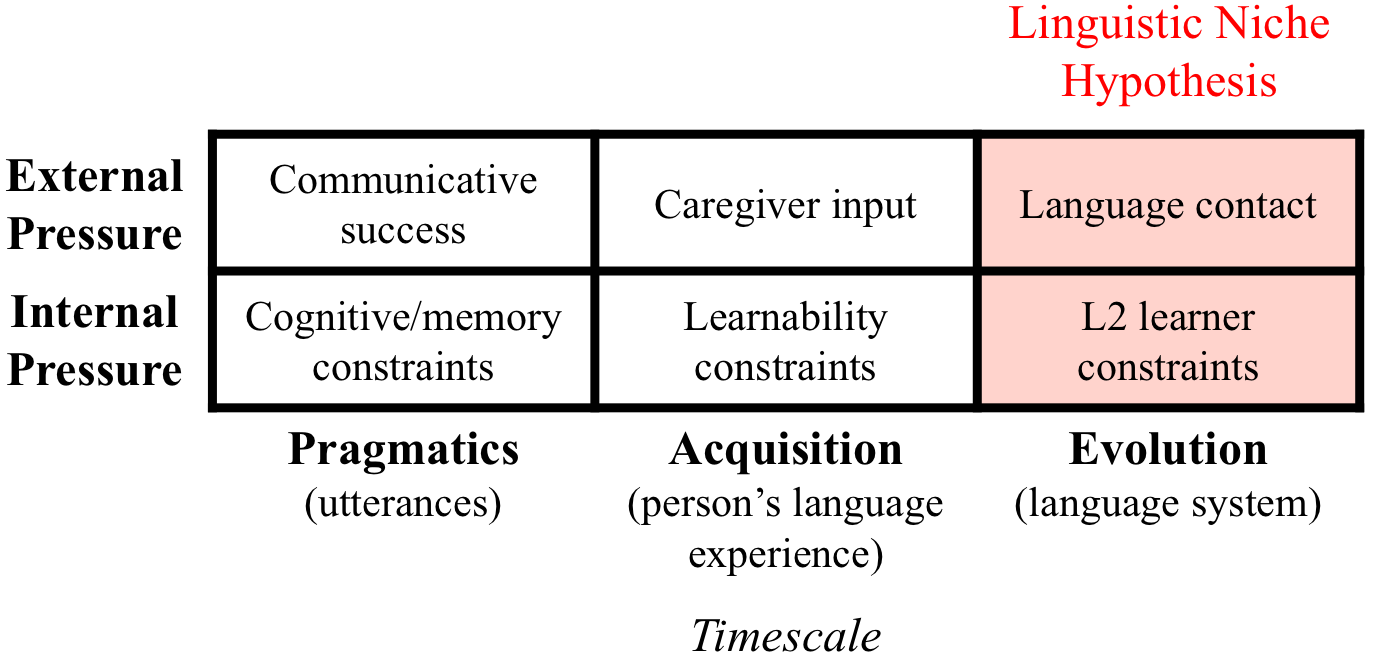
\includegraphics[scale = .34]{figs/timescales_table.png}
\end{center}
\caption{Pressures on language, internal and external to the cognitive system at three different timescales. The Linguistic Niche Hypothesis suggests that language evolution is influenced by the internal and external pressures in the particular environmental context in which a language is spoken.}
\label{fig:timescales}
\end{figure}

%An important aspect of this hypothesis is the timescale over which these pressures operate \cite{blythe2015hierarchy}. The central notion of a timescale is that there are different units of time over which different process operate, and that processes at shorter timescales influence those at longer timescale. For example, the language acquisition timescale operates over many years, but there is evidence that word learning is the product of communicative interactions at the pragmatic timescale (e.g., Baldwin, 1991; 1993; Frank, Goodman, \& Tenenbaum, 2009; Frank \& Goodman, 2014). There is also evidence that language systems may be the product of processes at the pragmatic timescale based on the observation that semantic spaces reflect optimal equilibria between pragmatic pressures. .

%An important aspect of this hypothesis is the timescale over which these pressures operate \cite{blythe2015hierarchy}. The central notion of a timescale is that there are different units of time over which different process operate, and that processes at shorter timescales influence those at longer timescale. For example, the language acquisition timescale operates over many years, but there is evidence that word learning is the product of communicative interactions at the pragmatic timescale (e.g., Baldwin, 1991; 1993; Frank, Goodman, \& Tenenbaum, 2009; Frank \& Goodman, 2014). There is also evidence that language systems may be the product of processes at the pragmatic timescale based on the observation that semantic spaces reflect optimal equilibria between pragmatic pressures. .




%But, why might languages differ from each other? That is, why might English Why Fig.1 

%(Regier, Kemp, & Kay, 2014; Kemp & Regier, 2012; Baddeley & Attewell, 2009) and aspects of the lexicon as a whole are also equilibria between these two pressures (Mahowald, Fedorenko, Piantadosi & Gibson, 2012; Lewis & Frank, 2014).

 %There are at least two scales at which language can be studied: individual utterances, which change over the course of moments in a communicative interaction, and language systems, which change over  the timescale of years.  An established body of work supports the claim  thats speakers adapt to the context at the scale of individual utterances, both in terms of the properties of the listener and the physical environment \cite<e.g.,>{schober1993spatial,frank2012predicting}. The present hypothesis explores the more controversial claim that environmental pressures shape language at the scale of language systems. %2x2 figure?

    

%This question can be considered at multiple timescales---the timescale of a single communicative interaction (pragmatics), a child's developmental trajectory (acquisition), or language evolution. At the timescale of pragmatics, theorists have suggested two pressures, one from the speaker (don't exert too much energy) and one from the communicative partner (get your message across).  Similarly, at the scale of acquisition, there are broadly two pressures: maturational constraints and input. In the present work, we explore the possibility that the same two pressures---one internal and one external to the cognitive system---shape language at the language evolution timescale. 

%Many facts about the social world are explicable only by considering the broader context: Why do gloves have five fingers? Why do tropical countries use lots of spices? The answers to these questions rely on taking into account properties of individual humans (hands have five fingers), and properties of the broader environmental context  \cite<tropical countries are hot, and spices kill bacteria;>{sherman1999darwinian}. 

%A growing body of work has begun to also explain {\it language structure} by  taking into account these same contextual factors.  systems. 




A number of recent studies provide correlational support for this proposal.  At the lowest level of the linguistic hierarchy, languages with larger populations are claimed to have larger phonemic inventories \cite{atkinson2011phonemic,hay2007phoneme}, but  shorter words \cite{wichmann2011phonological}. Speakers with more second language learners have also been suggested to have fewer lexical items \cite{bentz2015adaptive}. At the level of morphology, speakers with larger populations tend to have simpler morphology \cite{lupyan2010language,bentz2013languages}. Finally, there is also evidence that population size may influence the mappings between form and meaning. In particular, this work suggests that languages tend to map longer words to more complex meanings \cite{lewisstructure2014}, but that this bias is smaller for languages with larger populations  \cite{lewis_evolang}.

The plausibility of the Linguistic Niche Hypothesis depends largely on the presence of a possible mechanism linking environmental features to aspects of language systems. A range of proposals have been suggested \cite{nettle2012social}. For example, one possibility is that children (L1) and adult (L2) language-learners differ in their learning constraints. In particular, children may be better at acquiring complex morphology than adults, and so languages with mostly children learners may tend to have more complex morphology. A second possibility is that speakers in less dense social networks have less variable linguistic input, and this leads the language system to have more complex morphology.  

%The reported relationships between environmental features and linguistic features described above are efforts to test these hypotheses using available proxies.

Providing evidence for these mechanisms is empirically challenging, however. Because there are many factors that shape a linguistic system, large datasets are needed to detect a correlation with environmental factors. In addition, there is non-independence across languages due to genetic relationships and language contact, and so data from a wide range of languages are needed to control for these moderators \cite{jaeger2011mixed}. Third, the hypothesized mechanisms linking languages to their environments are somewhat underspecified. Finally, the large scale of this hypothesis makes it difficult to directly intervene on, and so we must rely primarily on correlational data to make inferences about mechanism.

%This is particularly problematic because the dynamics between these different factors may be complex, trading-off with each other in non-obvious ways \cite<e.g.,>{wichmann2011phonological}. 

 \begin{figure}[t!]
\begin{center}
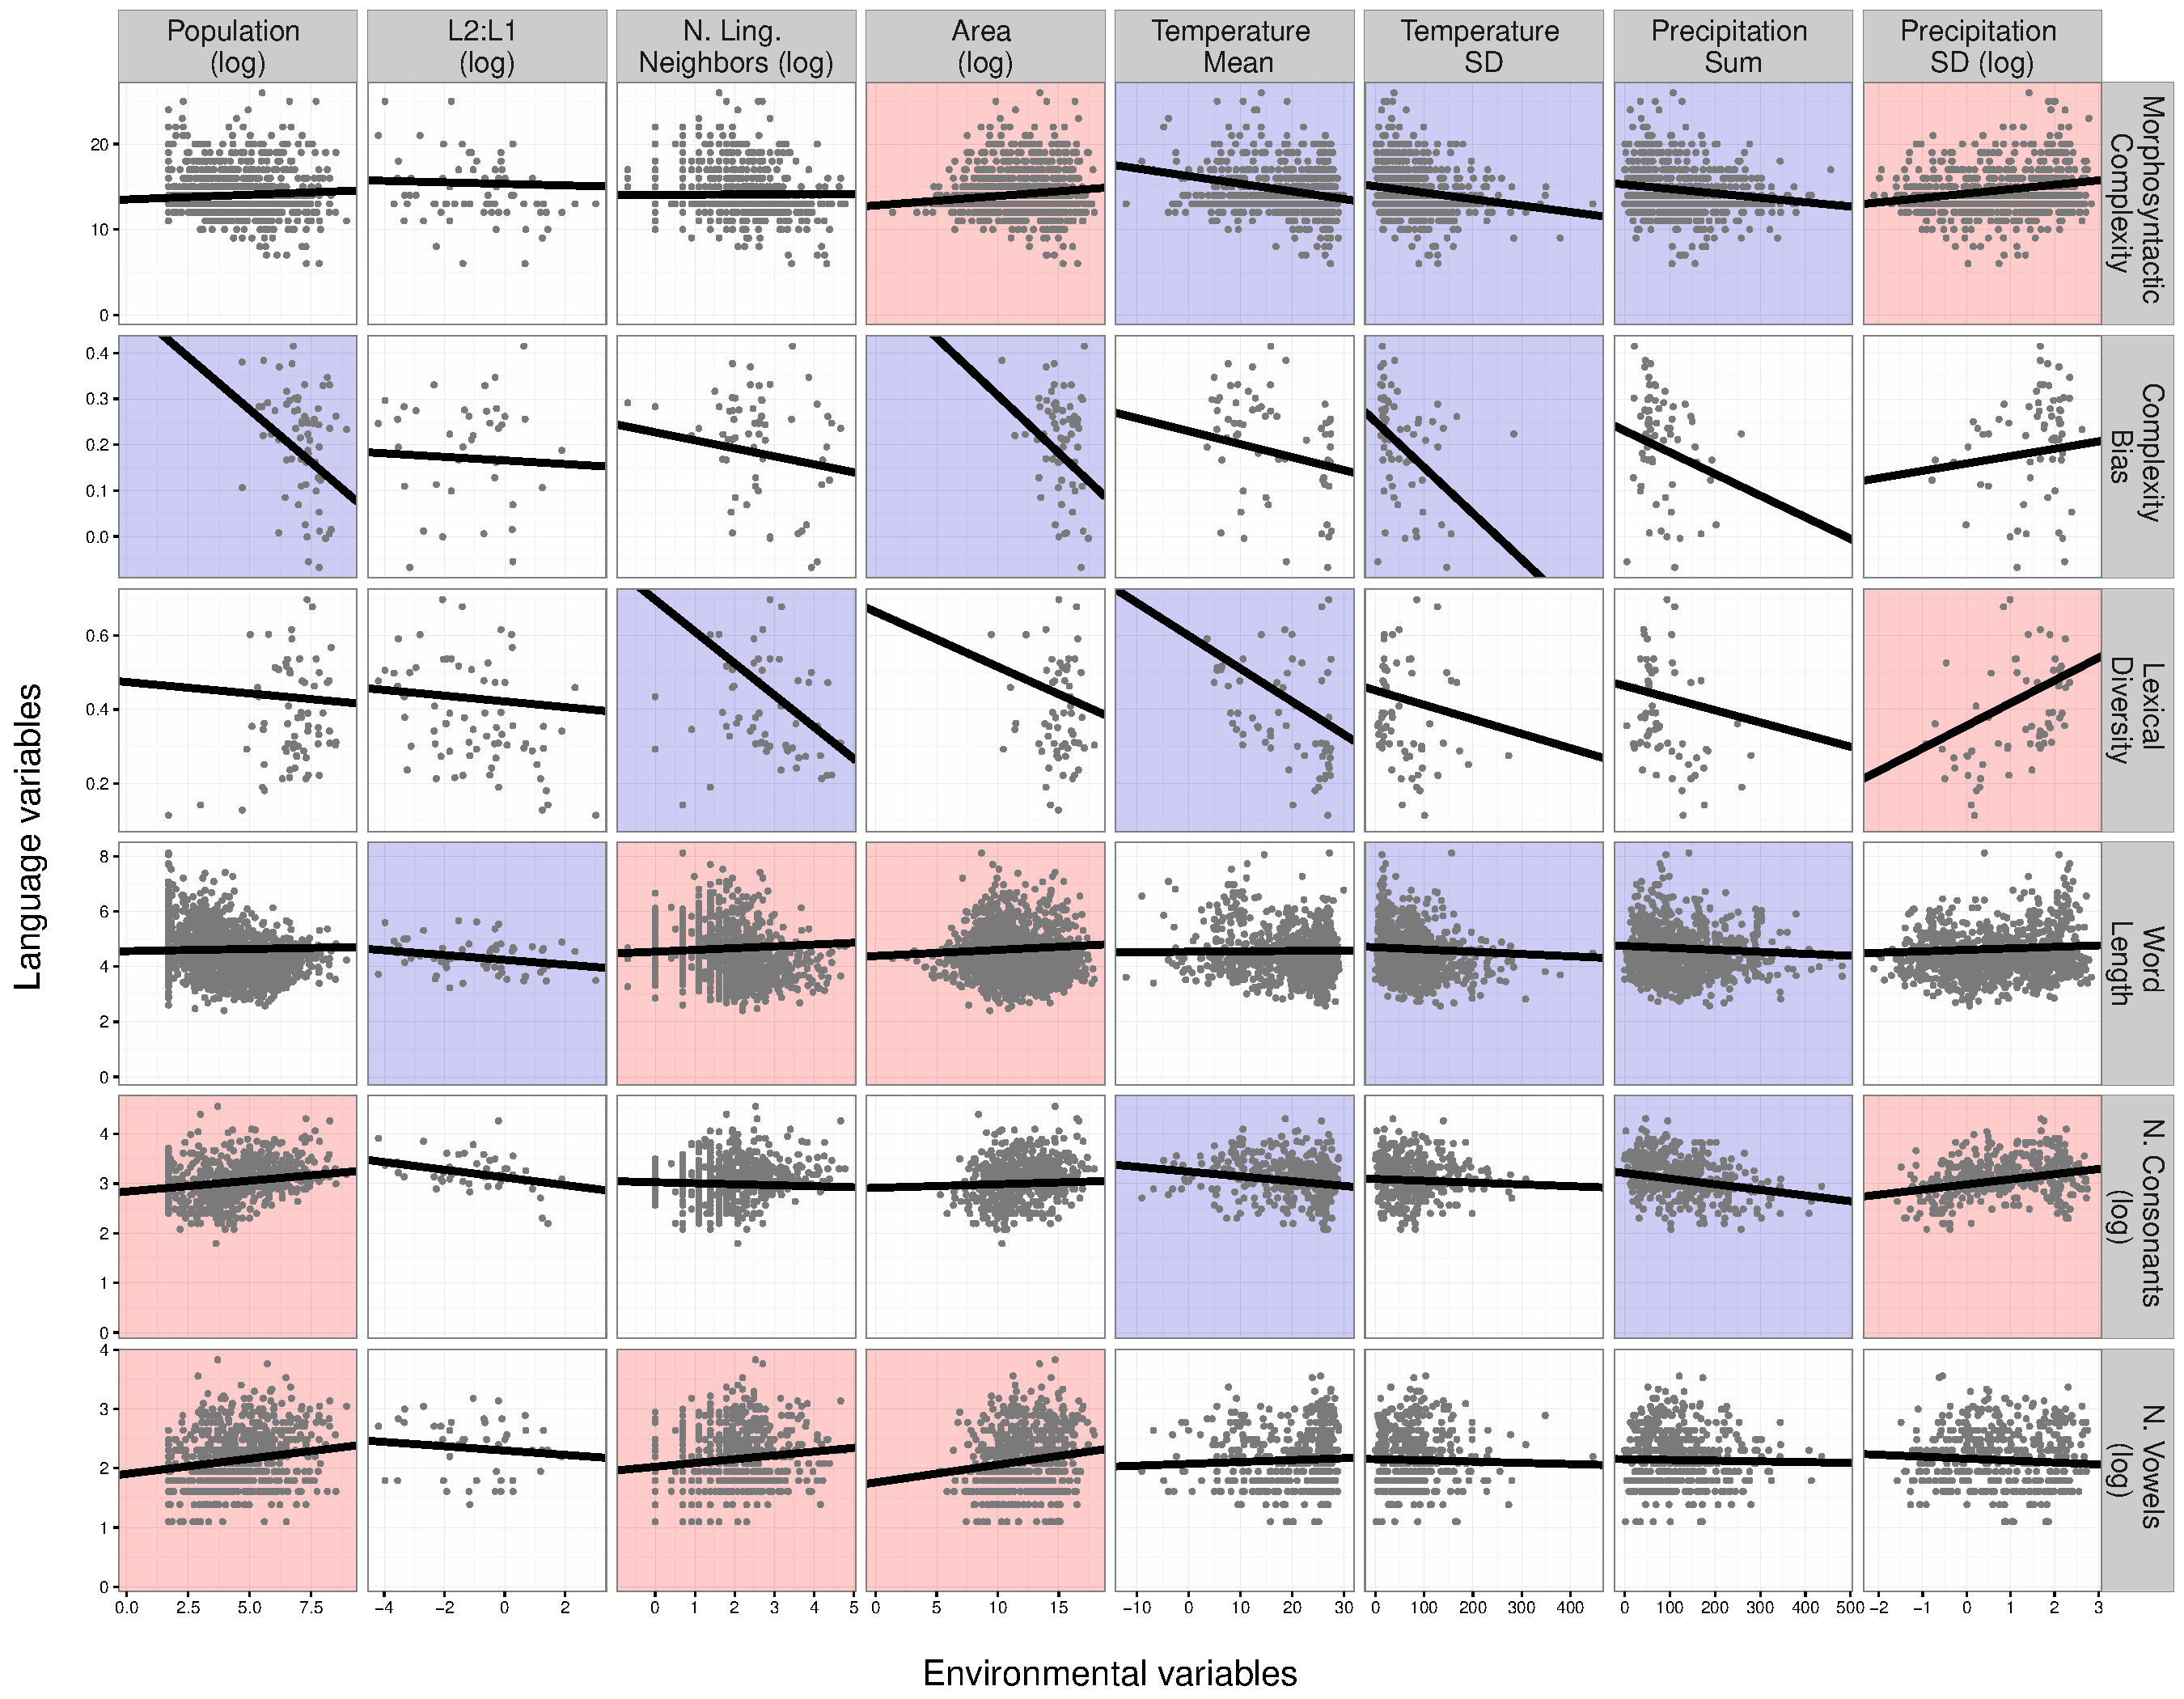
\includegraphics[scale = .33]{figs/plot_massive.pdf}
\end{center}
\caption{Relationship between environmental and linguistic variables, which each point represents a language. Red (positive) and blue (negative) indicate models where the environmental variable is a significant predictor of the linguistic variable. Lines show the fixed effect estimate (slope) and  intercept of the mixed effect model. Number of languages varies across plots due to variation in the number of overlapping languages across datasets.}
\label{fig:massive}
\end{figure}

In this work, we try to address some of these challenges by clarifying the empirical landscape. We do this by aggregating across datasets that find covariation between environmental variables and linguistic structure. This serves two purposes. First, it allows us to examine the relationship between the same set of environmental predictors across a range of linguistic features. And, second, it allows for the same analytical techniques and areal controls to be used across datasets. By addressing these inconsistencies, we are better able to  compare directly relationships between environmental and linguistic features. A more coherent picture of the empirical landscape may in turn provide insight into the mechanism linking language systems to their environments.

We also explore a novel aspect of the Linguistic Niche Hypothesis: the relationship between L1 and L2 learnability. We ask whether the same languages that are more easily learnable by second language learners are also easier to learn for first language learners, or whether there is some tradeoff in learnability. As a proxy a language's learnability for child-learners, we use the mean age of acquisition of children's first  words in a language. 

%For example, if  the correlation between environments and linguistic complexity is due to different learning constraints of L1 and L2 learners, then we should expect different kinds of languages to favor acquisition for different populations. We test whether languages thprediction that languages that are more easily learnable by L2 populations are harder to learn for L1 learners.

%We also more directly address the question of mechanism by examining variability in the mean age of acquisition of words for L1 learners across languages. Evidence that this variability is related to an aspect of the linguistic system (such as number of phonemes) would suggest that L1 learners, and not L2 learners, are the relevant environmental factor shaping that aspect of the linguistic system. 

In what follows, we first present a study examining the relationship between environmental and linguistic features using the same analytical techniques across all variables (Study 1). In Study 2, we examine the relationship between first language learnability and environmental and linguistic features.

%%%% Demo and language features%%%%%%
\section{Study 1: Environmental pressures on language}
The Linguistic Niche Hypothesis suggests that languages are shaped by their environment, but the exact nature of these effects has varied across the literature---both in terms of the variables considered and the direction of the effect. To explore this variation, we combined data from five existing datasets that included environmental or linguistic data. The datasets were selected for being publicly available and containing a large sample of languages. Below we describe each of these datasets, followed by our analytical methods, and results.

\begin{figure}[t]
\begin{center}
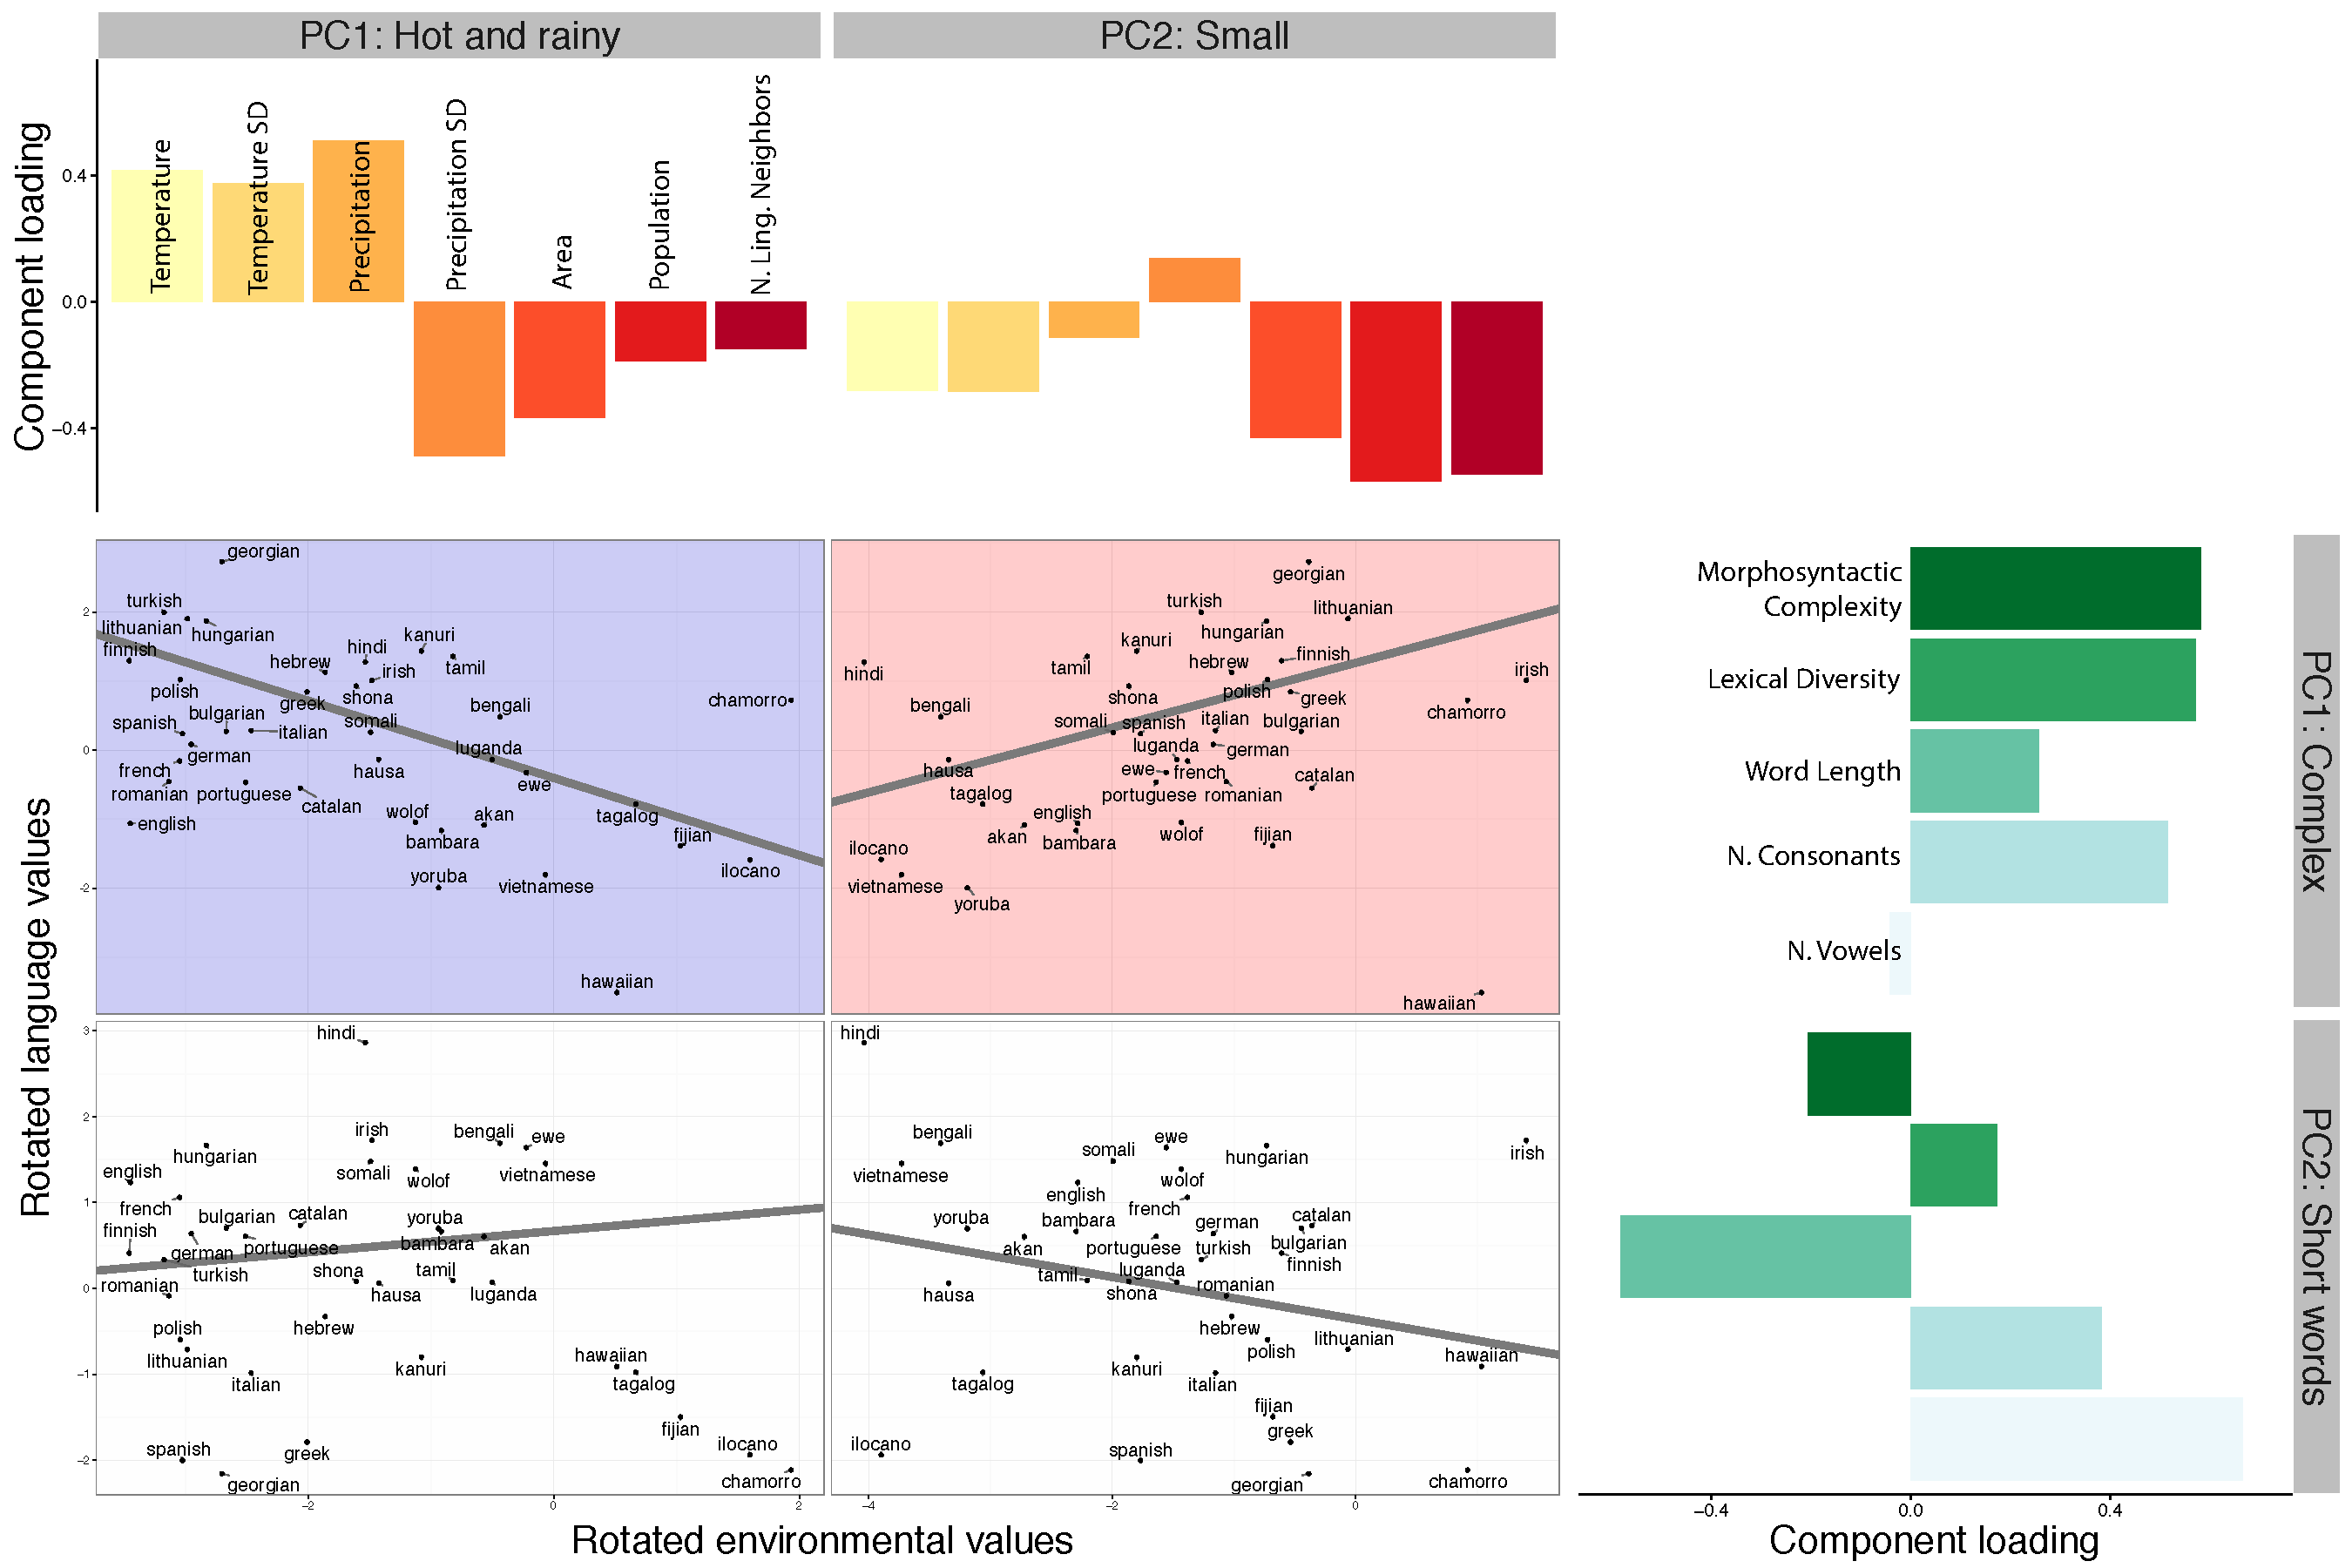
\includegraphics[scale = .3]{figs/plot2.pdf}

\end{center}
\caption{Languages spoken in cold, small regions tend to be more complex. The bar plots show the loadings on the first two principal components for the environmental variables ($n$ = 7; orange) and language variables ($n$ = 5; green). The scatter plots show the relationship between the first two principal components for both sets of variables. Each point corresponds to a language, and lines show the linear fit from the mixed effect model. Significance and direction of a linear relationship are indicated by the coloring of the scatterplot (blue: significant and negative; red: significant  and positive).}
\end{figure}

\subsection{Datasets}
{\it Lupyan and Dale (2010).} This dataset contains grammatical information from WALS \cite{wals}, and demographic and geographic information from Ethnologue and the Global Mapping Institute \cite{gordon2005}. The demographic and geographic variables included total population of speakers, number of neighboring languages, area of region in which the language is spoken ($km$\textsuperscript{2}), mean and standard deviation temperature ($celsius$), and mean and standard deviation precipitation ($cm$). We used these data to create a metric of morphosyntactic complexity calculated from  27 of the 28 morphosyntactic variables analyzed in the original paper.\footnote{WALS variable 59 was missing from the dataset.}  For each variable, we coded the strategy as simple if it relied on a lexical strategy or few grammatical distinctions (e.g.,  0-3 noun cases), and complex if it relied on a morphological strategy or many grammatical distinctions (e.g.,  more than 3 noun cases). We summed the number of complex strategies to derive a measure of morphosyntactic complexity for each language, including only languages with data for all 27 variables\footnote{We would like to thank Gary Lupyan and Rick Dale for sharing their data with us.}. [$n$ = 1991 languages] 
%\cite{gmi}

{\it Bentz et al.\ (2015).} Two variables were used from this dataset: ratio of L2 to L1 speakers and number of word forms. Estimates of number of word forms were taken from translations of the  {\it Universal Declaration of Human Rights}. Number of word forms was calculated as the number of unique words divided by the number of total words (type-token ratio). Higher type-token ratio indicates more word types in that language. Speaker population data were taken from a variety of sources, where L2 speakers were restricted to adult non-native speakers only. [$n$ = 81]

{\it Moran, McCloy and Wright (2012).} Estimates of number of consonants and vowels in each language were used from this dataset. [$n$ = 969] 

{\it Lewis and Frank (2014).} This work finds that languages tend to map more complex meanings (measured via semantic norms) to longer words. The bias is estimated as the correlation (Pearson's $r$) between word length and complexity ratings for a set of 499 words translated via Google Translate. We used estimates of the correlation that partialed out the effect of spoken frequency. [$n$ = 79]

{\it Wichmann, Rama, and Holman (2014).} This database contains translations for 40-lexical items across many languages. Word length was calculated as the mean number of characters in the ASJPcode transcription system across words in each language. [$n$ = 4421]

Aggregating across datasets, we analyzed 8 environmental variables in total: L2-L1 population ratio, total population size, number of neighbors, area of spoken region, mean and standard deviation temperature, and mean and standard deviation precipitation. These variables were selected from a larger set because they were not highly correlated with each other ($r<.8$). We analyzed 6 total linguistic variables: number of vowels, number of consonants, word length, type-token ratio, complexity bias, and morphosyntactic complexity.

\subsection{Method}
Datasets were merged using common ISO-639 codes when available. Five variables were log-transformed to better approximate a normal distribution (population, L2 to L1 ratio,  number of neighbors, area, number of consonants, number of vowels).\footnote{All code and data for the paper are available at \url{http://github.com/mllewis/langLearnVar}} 

\subsubsection{Main analysis}
We  tested for a linear relationship between each environmental and language variable.  A significant challenge in making inferences about language data is non-independence. This non-independence can come from at least two sources: genetic relatedness and language contact. Following \citeA{jaeger2011mixed}, we control for these factors statistically by using linear mixed-effects regression. We control for genetic non-independence by including a random intercept and slope by language family. We control for language contact by including country of origin as a random intercept (models with random slopes failed to converge).\footnote{The model specification was as follows:  \texttt{language.variable $\sim$ environmental.variable + (environmental.variable~\textbar~language.family) +  (1~\textbar~origin.country)}.}  We selected country of origin as a proxy for linguistic community because it was available for all languages in our dataset. Both control variables were taken from the WALS dataset. We considered a predictor significant if the test statistic on the fixed effect coefficient exceeded 1.96. 

\subsubsection{Principal component analysis}
This first analysis provides a uniform analysis of the many environmental and linguistic variables that have been used to test the Linguistic Niche Hypothesis. However,  the large number of variables makes it difficult to distill a coherent picture from these data. Given that many of these variables are partially correlated with each other, we used a technique for reducing the dimensionality of the dataset---principal component analysis. We found the principal components associated with the variance for the environmental variables and the linguistic variables, and then fit the same model as in the primary analysis using the rotated values. Complexity bias was excluded because it was only available for a small subset of languages.  All variables were scaled.  

\subsection{Results}
In the main analysis, we fit mixed effect models predicting each language variable with each environmental variable using areal controls. The results are presented in Figure 5.2. For each language variable, there was at least one environmental variable that reliably covaried, though some previously-reported effects were not significant in this analysis. We return to this in the discussion. Data can be explored interactively here: \url{https://mlewis.shinyapps.io/lhnn/}.

The principal component analysis revealed two primary components of variance for both the environmental and linguistic variables. For the environmental variables, the first two principal components accounted for  .69 of the total variance (PC1: .39; PC2: .30).  The weights on these variables across the two components can be seen in the upper panel of Figure 5.3. The first component  loads most heavily on variables related to the climate. It can be thought of as corresponding to hot and rainy regions. The second component loads most heavily on variables related to the size of the region a language is spoken in, both in terms of number of speakers and physical size. This principal component can be roughly interpreted as the `smallness' of a linguistic community.

For the linguistic variables, the first two components also accounted for most of the variance, .70 (PC1: .39; PC2: .31; right panel of Fig.\ 3). The first component loads positively on all variables, except number of vowels. In particular, this component is associated with more consonants, longer words, more word types, and greater morphosyntactic complexity. Broadly, this component is related to the amount of cognitive difficulty associated with learning a language. The second component is associated with having short words, but large phonemic inventories. 

Figure 3 shows the relationship between the principal components. Both environmental principal components were reliable predictors of the first linguistic principal component (PC1: $\beta=-0.56$, $t=-3.52$; PC2: $\beta=0.47$, $t=2.08$). This suggests that languages that tend to be  spoken in cold and small regions are more likely to be more complex. Neither of the environmental principal components were reliable predictors of the second linguistic principal component.

\subsection{Discussion}
These two analyses suggest that more complex languages are spoken in cold, small regions. Importantly, we find this relationship across a range of linguistic features---morphosyntactic complexity, linguistic diversity, word length, and consonant inventory---using the same analytic technique across all measures. 

This finding is broadly consistent with previous work that finds relationships between  individual metrics of complexity and various demographic variables. Nevertheless, we find null effects for several reported relationships in the literature. For example, the relationship between population size and morphosyntactic complexity  \cite{lupyan2010language} is not reliable in our model with areal controls, though the correlation is significant ($r$ =.08; $p<$.001) and we replicate their finding in a binned analysis (Fig. 5.3 of Lupyan \& Dale, 2010).  There are many possible reasons for these differences (e.g., different measure of complexity, different areal controls), highlighting the need for a common analytical approach across  datasets.

Why might languages in small, cold regions have more complex languages? One possible mechanism is  that languages spoken in larger places have more L2 learners, and that L2 learners are less skilled than L1 learners at acquiring complex language. As a result, these languages adapt by simplifying. The relationship between climate and linguistic complexity is less clear, but one possibility is that  speakers in  colder regions are less itinerant, and therefore have less contact with adult speakers of other languages.

%%%% AOA %%%%%%
\section{Study 2: Variability in L1 learning}
The proposed mechanism in Study 1 makes an important assumption: L2 learners, but not L1 learners, are poor learners of linguistic complexity.  \citeA{lupyanrole} have argued that morphological complexity in fact {\it facilitates} learning for L1 learners by providing redundancy in the linguistic signal. A straightforward prediction of this hypothesis is that languages that are more easily learnable by L2 learners will be less learnable by L1 learners. 

In Study 2, we explore this prediction. As a proxy for language learnability for L1 learners, we use the mean age of acquisition (AoA) of words in a language by L1 learners (children).  If there is a tradeoff between learnability for L1 and L2 learners, languages that are less complex should be harder for children to learn, and thus have later AoAs.

\subsection{Method}
We use subjective measures of AoA from the the \citeA{luniewska2015ratings} norms. These AoAs were collected from adult participants for the translation equivalents of 299 words in 25 languages. To evaluate the validity of this measure, we compared these ratings to more objective measures of AoA collected from parent-report using the CDI \cite<Wordbank;>{frankwb}.  We fit a model predicting the objective ratings with the subjective ratings for the small sample of common languages ($n=7$). We included language as a random by-intercept and by-slope effect. Subjective ratings were a strong predictor of objective ratings ($\beta=1.00$, $t=5.45$), suggesting that the  \citeA{luniewska2015ratings} norms were a reasonable proxy for cross-linguistic AoA.
% or just correlaiotn: .36

We averaged across words in the \citeA{luniewska2015ratings} database to get a mean AoA for each language. We then used the same mixed-effect model as in Study 1 to predict AoAs with each of the linguistic and environmental variables analyzed in Study 1. 

\subsection{Results}
Number of consonants positively predicted AoA, suggesting that languages with more consonants tend to have later AoAs ($\beta=1.04$, $t=1.97$). In addition, temperature positively predicted   AoA ($\beta=.13$, $t=2.57$) and variability in precipitation negatively predicted AoA ($\beta=-1.6$, $t=-2.83$). No other variables were significant predictors of AoA. 

\subsection{Discussion}
Study 2 explores a prediction about a mechanism for the relationship between population size and linguistic complexity: L1 learning is facilitated by complexity in the linguistic signal (via redundancy), but L2 learning is hindered. We find only limited support for this proposal. Of the factors that loaded on ``complexity"  in the principal component analysis in Study 1, number of consonants was the only reliable predictor of AoA. 

Nevertheless, we do find several surprising correlates of AoA---number of consonants, temperature, and precipitation variability---even in this very small sample of languages. The mechanism underlying these relationships is not clear. It could be for example that L1 learners in colder regions have more language input, and therefore earlier AoAs. Or, if we assume that temperature and variability in precipitation are proxies from L2 pressure (as suggested in Study 1), it could be that languages with more L2 pressure have later AoAs, and therefore are harder for L1 learners to acquire. A larger sample of languages will be needed to address these questions.

\section{Conclusion}
Languages vary in many ways across multiple timescales of analysis. Here we suggest that this variability can be accounted for by considering the relationship between these timescales and two types of pressures, those internal and external to the cognitive system. In the present work, we have explored a hypothesis at the language evolution timescale---the Linguistic Niche Hypothesis---which suggests that cross-linguistic variability is the result of different cognitive constraints of learners and  environmental pressures.

We contribute to the empirical findings related to this hypothesis by synthesizing previous correlational evidence using common analytical techniques across datasets. Across a range of linguistic and environmental metrics,  we find that more complex languages tend to be spoken in smaller, colder regions. We also find evidence  that the learnability of a language for L1 learners may be related to aspects of the language (number of consonants) and the environment (temperature and variability in precipitation). Understanding  how   {\it both} child and adult learners shape language systems is an important question for future work. 

Accounting for variability at the timescale of language evolution is an empirically challenging enterprise. Moving forward, we suggest that a fruitful avenue for progress is holistic descriptions of the empirical landscape, and appeals to processes at multiple timescales of analysis.


%Dale and luypan -- more stringent controls (monte carlo sampling in 2010 paper)

%Informative about the origins of language (~devo)
%Other attempts to get at this quesiton (modeling + experimental)
%Why? Cold and complex
%using Monte Carlo analyses to deal with Galton�s problem of non-independent sampling; Lupyan & Dale, 2010

%L2 vs. L1 learners might be good at different things


%\cite{silvey2015word}
%\cite{perfors2011language}




%\cite{wichmann2011phonological}
%\cite{wichmann2008languagephonological}
%\cite{smith2010eliminating}
%\cite{slobin1982children}

%\cite{sapir1912language}
%\cite{reali2014paradox}




%\cite{lupyan2010language}
%This proposal is relatively uncontroversial at the level of semantics \cite{sapir}: Languages have words for meanings that are relevant for their environment (e.g. ). But, at  more abstract levels of language structure, this hypothesis has been very controversial. 
%\cite{kirby2008cumulative}
%Meaning. \cite{silvey2015word}
%\cite{perfors2011language}
%Critically, 

% Moran et al., 2012) 
\nocite{moran2012revisiting}







%!TEX root = ../dissertation.tex

\chapter{Conclusion}
\label{chapter:conclusion}
Important concluding remarks.

motivation was pragmatics -> not necessarily pragmatics (chapt 4) just stuff at smaller timescales.
dynamics between pressures

deal with pragmatic vs. in-the-moment issue

 (about 5 pgs)
Discussion of limitations
Future directions


%\appendix
%\chapter{A Long Proof}

\bibliographystyle{apacite}
\bibliography{dissertation}

\end{document}